This section contains experimental results from the experiments conducted to find the best possible price predicting solution. The experiments are based on the data which we have analysed in section \ref{sec:ElectricityPriceAnalysis}. The experiments are done to validate whether the assumptions about the input parameters are true when used in an Feedforward Neural Network. We also examine the best combinations to find the most optimal solution for price prediction. The results are divided into five experiments. The first experiment finds the best combination of input parameters for the network. These input parameters count meteorological, social and seasonal factors --- which we identified in the analysis section~\ref{sec:Price}. The next experiment identifies the need for trimming and reasons to why it is needed in this particular dataset. The third experiment tests how different calculated inputs can include the immediate historical curve behavior in the dataset. This includes scatter, slope calculation, skewness analysis and historical EWMA (Exponentially-Weighted Moving Average). The fourth experiment takes care of the Feedforward Neural Network parameters called black-box optimization. The last experiment shows the influence of offsets for the prediction and the effect of limiting the hours-ahead used in the predictions.

The purpose of these experiments are to identify the best parameters, data manipulation, calculated inputs and black box optimizations. This is done through a series of experiments that either validates or rejects the hypothesis set up in each experiment. We want to approach the target price but the main focus is to test what works and what does not work regarding the electricity price predictions.

\subsection{Experiment One - Selection of input parameters}
\label{sec:priceExperimentOne}
This section is based on the input parameters that we identified in section~\ref{sec:Price}. We have done a cross comparison of all the inputs and possible combinations. The last known price and the predicted demand are basic measures when you define a price in any market and that is why we include them in every prediction. We have not made a cross comparison of the Month of Year and the Seasons of Year since they denote the same but with different granularity. We have done a cross comparison both with and without matrix inputs and with a mix of non-matrix and matrix inputs. This is done to determine whether an input makes better sense on matrix form or just as a simple normalized value. This is a difference from wind power experiments (that first identified inputs and applied matrix afterwards) but it is done here because the amount of possible matrices is higher. 

\subsubsection{Variables}
Experiment one is based on a dataset consisting of the last three months averaging to 2189 hours. We use 200 epochs for each training iteration.

The parameters being examined in this test are the following:
\begin{enumerate}
	\item Last Hours Price (P)
	\item The Demand (D)
	\item Wind Speed(WS)
	\item Temperature(T)
	\item The Hourly Time of Day (ToD)
	\item The Day of the Week(DoW)
	\item The Month(Mo)
	\item The Season of the Year(SoY)
\end{enumerate}

The (m) is for Matrix input and states if the input in the time-related rows(ToD, WoD, MoY, SoY) are represented as a matrix.

The table~\ref{table:Top20Prices} contains the following information as well:
\begin{enumerate}
	\item Number in table (\#)
	\item First hidden layer neuron count (H1)
	\item Second hidden layer neuron count (H2)
	\item How many percent of the predictions follows the curve movement in the correct direction (\% CD)
	\item \% ranking from first entry (\% Rank)
	\item Mean Average Error (MAE)
\end{enumerate}

\subsubsection{Hypothesis}
This is the first and most comprehensive of the tests conducted for price prediction. In this experiment we want to test all of the different input parameter combinations. We expect to see a better curve-fit as we include more variables and more complex variables. In regards to the dataset analysis in section~\ref{sec:ElectricityPriceAnalysis} we see the connection between the aforementioned variables and the price. We have the following expectations based on the dataset analysis:
\begin{enumerate}
	\item The Wind Speed will show a positive impact on the price because of the correlation between the two. Also the wind speed impacts the production of green energy which impacts the overall price of energy. Since the wind power production accounts for about 25\% (see data analysis in section ~\ref{sec:Price}) of the complete power production in western Denmark we also expect to see that this parameter will increase accuracy.
	\item The Temperature might have a small impact on the price but there is nearly no correlation between the price and the temperature. If it should have an impact it is because of the correlation between the temperature and the demand thus indirectly influencing the price.
	\item The Hourly Time of Day is expected to have an effect on the hourly predicted price. The reason being the correlation between the price and the time of day and because we are predicting the hourly price; which logically indicates that this parameter is important for such a prediction. 
	\item The Day of the Week, The Month of the Year and The Seasons of the Year is expected to have a positive impact on the prediction. The impact are expected to get smaller as the inputs become more general e.g season of year; since our training dataset is based on 1/4 of a year. 
	\item Matrix representation will be better than single node representation of the seasonality. This is due to the fact that matrix is a more granulated input format than single node. This has also been discussed in section~\ref{sec:Matrix}.
\end{enumerate}

\subsubsection{Results}
We present the results from this experiment in table~\ref{table:Top20Prices}. The input parameters will be analysed one by one in the next subsections. After that we will discuss some of the problems with selected input parameters.

\begin{table}[H]
\centering  % used for centering table
\resizebox{\textwidth}{!}{
\begin{tabular}{|c|c|c|c|c|c|c|c|c|c|c|c|c|c|} % centered columns (7 columns)
\hline
{\#} & P & D & WS & T & ToD & DoW & Mo & SoY & \% CD & H1 & H2 & MAE & {\%} Rank \\ [0.5ex] % inserts table 
%heading
\hline                  % inserts single horizontal line
1  &  \x    & \x    & \x    & \x    & \x\m  & \x\m  &       & \x\m  & 66,8\% &  7  & 8  & 57,12 & - \\ \hline
2  &  \x    & \x    & \x    & \x    & \x\m  & \x    &       & \x\m  & 67,9\% &  5  & 9  & 58,09 & 1,7\% \\ \hline
3  &  \x    & \x    & \x    & \x    & \x\m  &       & \x\m  &       & 66,5\% &  6  & 11 & 58,79 & 2,92\% \\ \hline
4  &  \x    & \x    & \x    &       & \x\m  & \x\m  & \x\m  &       & 66,5\% &  9  & 3  & 60,14 & 5,29\% \\ \hline
5  &  \x    & \x    & \x    & \x    & \x\m  & \x    &       &       & 66,9\% &  16 & 8  & 62,19 & 8,88\% \\ \hline
6  &  \x    & \x    & \x    & \x    & \x\m  &       &       & \x\m  & 67,2\% &  6  & 5  & 62,26 & 9,0\% \\ \hline
7  &  \x    & \x    & \x    & \x    & \x\m  & \x    & \x\m  &       & 67,0\% &  5  & 8  & 62,84 & 10,01\% \\ \hline
8  &  \x    & \x    & \x    & \x    & \x    & \x    &       & \x\m  & 62,9\% &  5  & 0  & 63,94 & 11,94\% \\ \hline
9  &  \x    & \x    & \x    & \x    & \x    & \x\m  & \x\m  &       & 62,2\% &  5  & 4  & 64,19 & 12,38\% \\ \hline
10 &  \x    & \x    & \x    &       & \x\m  & \x    & \x\m  &       & 67,4\% &  6  & 8  & 64,72 & 13,31\% \\ \hline
11 &  \x    & \x    & \x    &       & \x    & \x    & \x\m  &       & 63,3\% &  5  & 5  & 65,07 & 13,92\% \\ \hline
12 &  \x    & \x    & \x    & \x    & \x\m  & \x\m  &       &       & 67,0\% &  6  & 6  & 65,95 & 15,46\% \\ \hline
13 &  \x    & \x    & \x    & \x    & \x\m  & \x\m  & \x\m  &       & 66,8\% &  7  & 12 & 66,55 & 16,51\% \\ \hline
14 &  \x    & \x    & \x    &       & \x    &       &       & \x\m  & 62,4\% &  7  & 0  & 67,21 & 17,66\% \\ \hline
15 &  \x    & \x    & \x    & \x    & \x    & \x    &       &       & 62,6\% &  5  & 0  & 67,88 & 18,84\% \\ \hline
16 &  \x    & \x    & \x    &       & \x    & \x    &       & \x    & 62,0\% &  6  & 0  & 68,21 & 19,42\% \\ \hline
17 &  \x    & \x    & \x    &       & \x\m  & \x\m  &       &       & 67,2\% &  8  & 6  & 68,34 & 19,64\% \\ \hline
18 &  \x    & \x    & \x    &       & \x\m  &       &       & \x\m  & 68,2\% &  7  & 4  & 68,35 & 19,66\% \\ \hline
19 &  \x    & \x    & \x    & \x    & \x    & \x    & \x    &       & 62,2\% &  6  & 0  & 68,43 & 19,8\% \\ \hline
20 &  \x    & \x    & \x    & \x    & \x    &       &       & \x\m  & 62,4\% &  5  & 0  & 68,45 & 19,84\% \\ \hline
\end{tabular}
}
\caption{The top 20 results on training set 3 last months} % title of Table
\label{table:Top20Prices} % is used to refer this table in the text
\end{table}

\subsubsection{Wind speed}
If we take a look at the top 20 best input combinations (shown in Table~\ref{table:Top20Prices}) we can observe clear trends. We will start by analysing the data from left to right. The price and demand are as mentioned earlier static since they are fundamental market forces and thus not a changing factor in this analysis. The next input parameter is the Wind Speed. We see that every input combination in the top 20 includes the wind power and it is therefore a must for the prediction of the energy prices. Actually the 72 first inputs (the 50\% best results) contains only two combinations that does not have wind speed in them. Also we saw in section~\ref{sec:windPowerAnalysis}(table~\ref{table:pearsonCoeficientWindProduction}) that the Wind Speed heavily influences the wind power and thus influencing the energy prices. If we remove wind speed from the \#1 combination it ends up at place \#70 which are 37.55\% worse than the best result. In Figure~\ref{fig:Windspeed_no_windspeed} we see that the prediction without wind speed has a tendency to overshoot more than the one with wind speed does (the dark overlays shows where it overshoots). Over a whole year this sums up to a significant difference.

\begin{figure}[H]
\centering
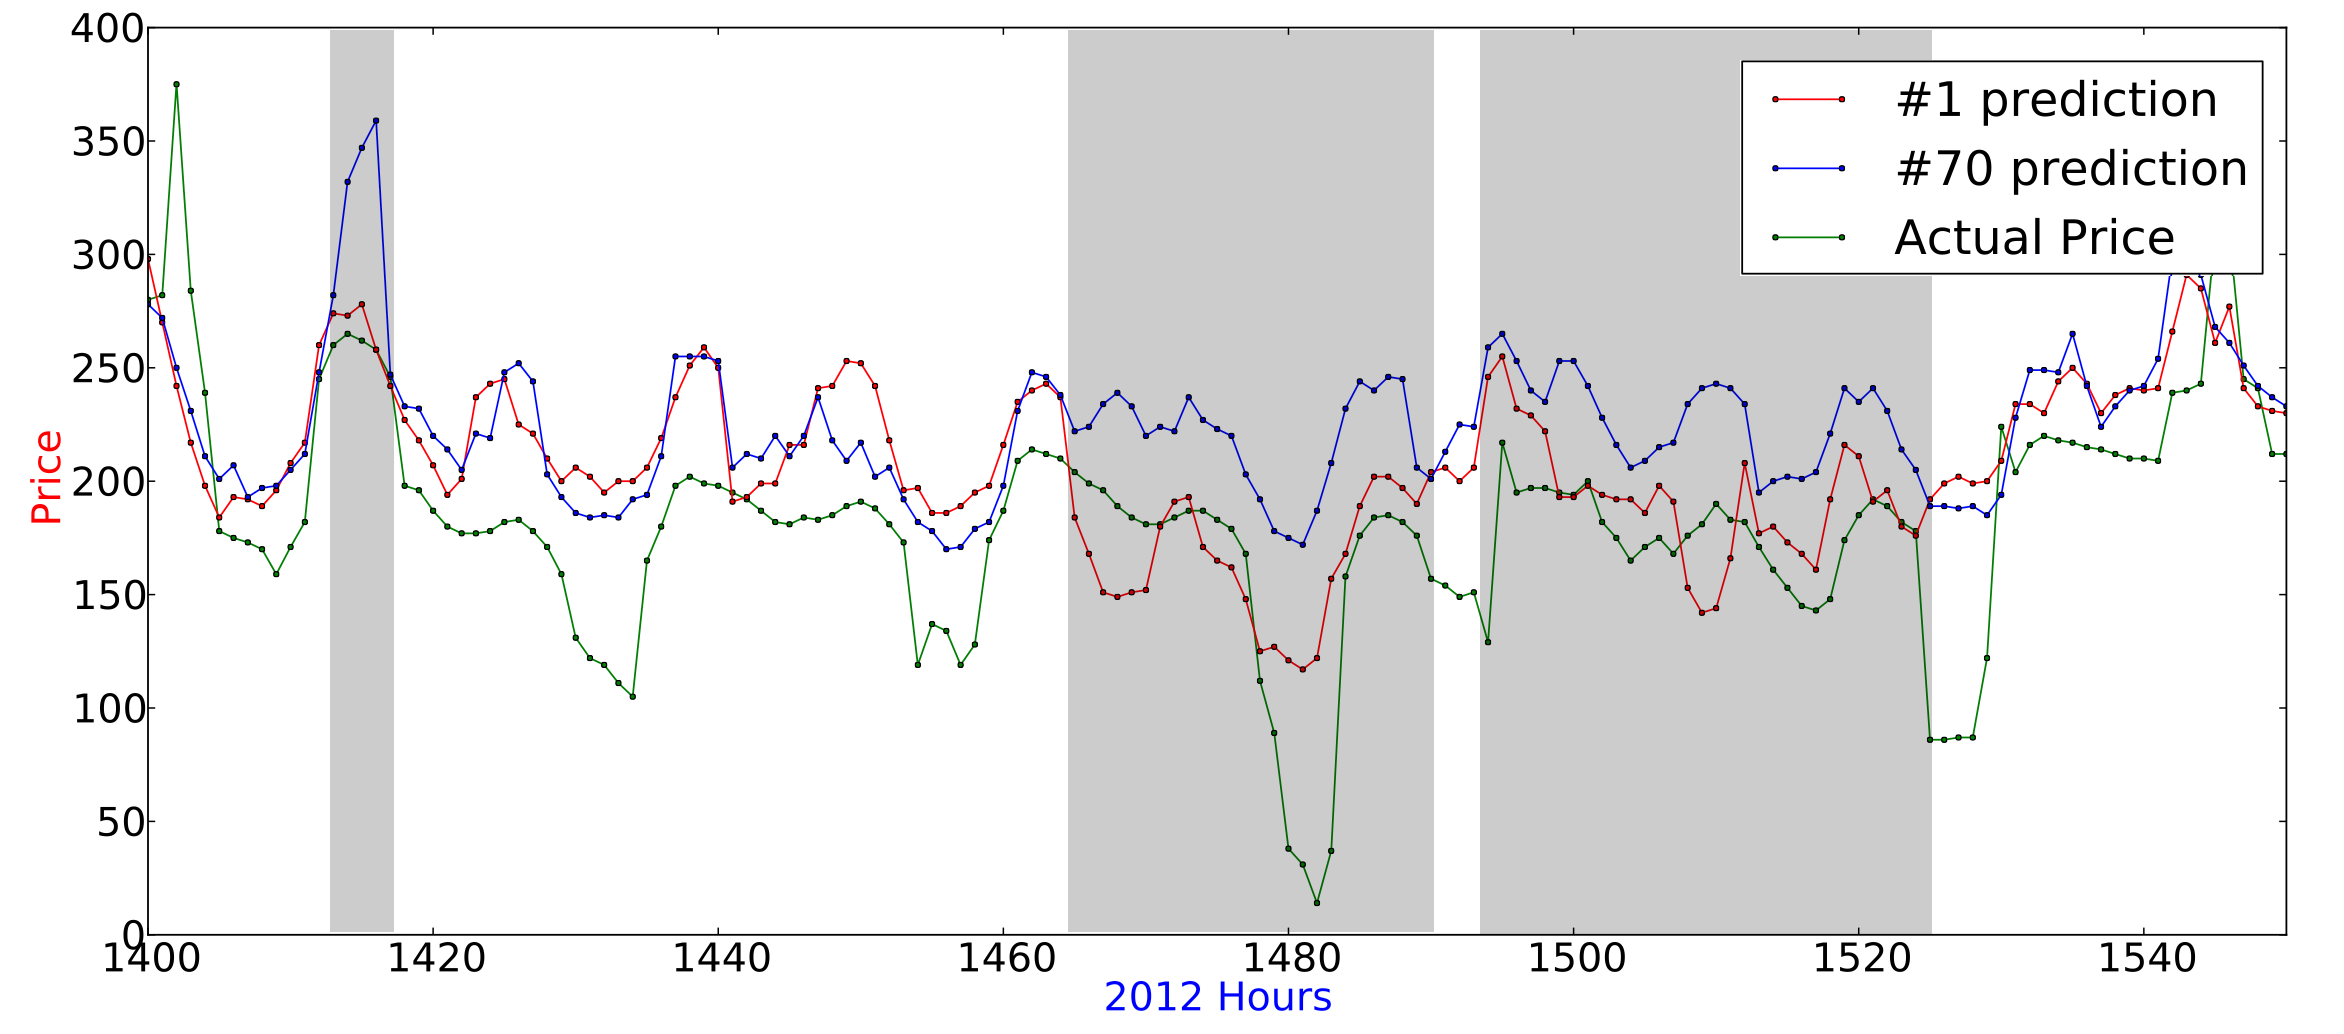
\includegraphics[width=\linewidth]{billeder/PriceExperimentalAnalysis/X1_windspeed_vs_no_windspeed.png}
\caption{\#1 forecast from table~\ref{table:Top20Prices} with and without wind speed}
\label{fig:Windspeed_no_windspeed}
\end{figure}

\subsubsection{Temperature}
The temperature is a less obvious candidate for the prediction of price since the Pearson's correlation between the two only are 0.17. Nevertheless it is showing up in 8/10 top combinations in Table~\ref{table:Top20Prices} and this might be because of the correlation between temperature/demand which is -0.59. The temperature is scattered all over the 144 combinations and thus it is hard to say something concrete about this input variable. The best result without temperature is at place 4 in Table~\ref{table:Top20Prices} and the same one with temperature is at place 13 with a difference between the two of 10.66\%. Graph~\ref{fig:temperature_comparison} shows that there is no significant difference between the two combinations. In both of them the ANN is overshooting the target at different spots.

\begin{figure}[H]
\centering
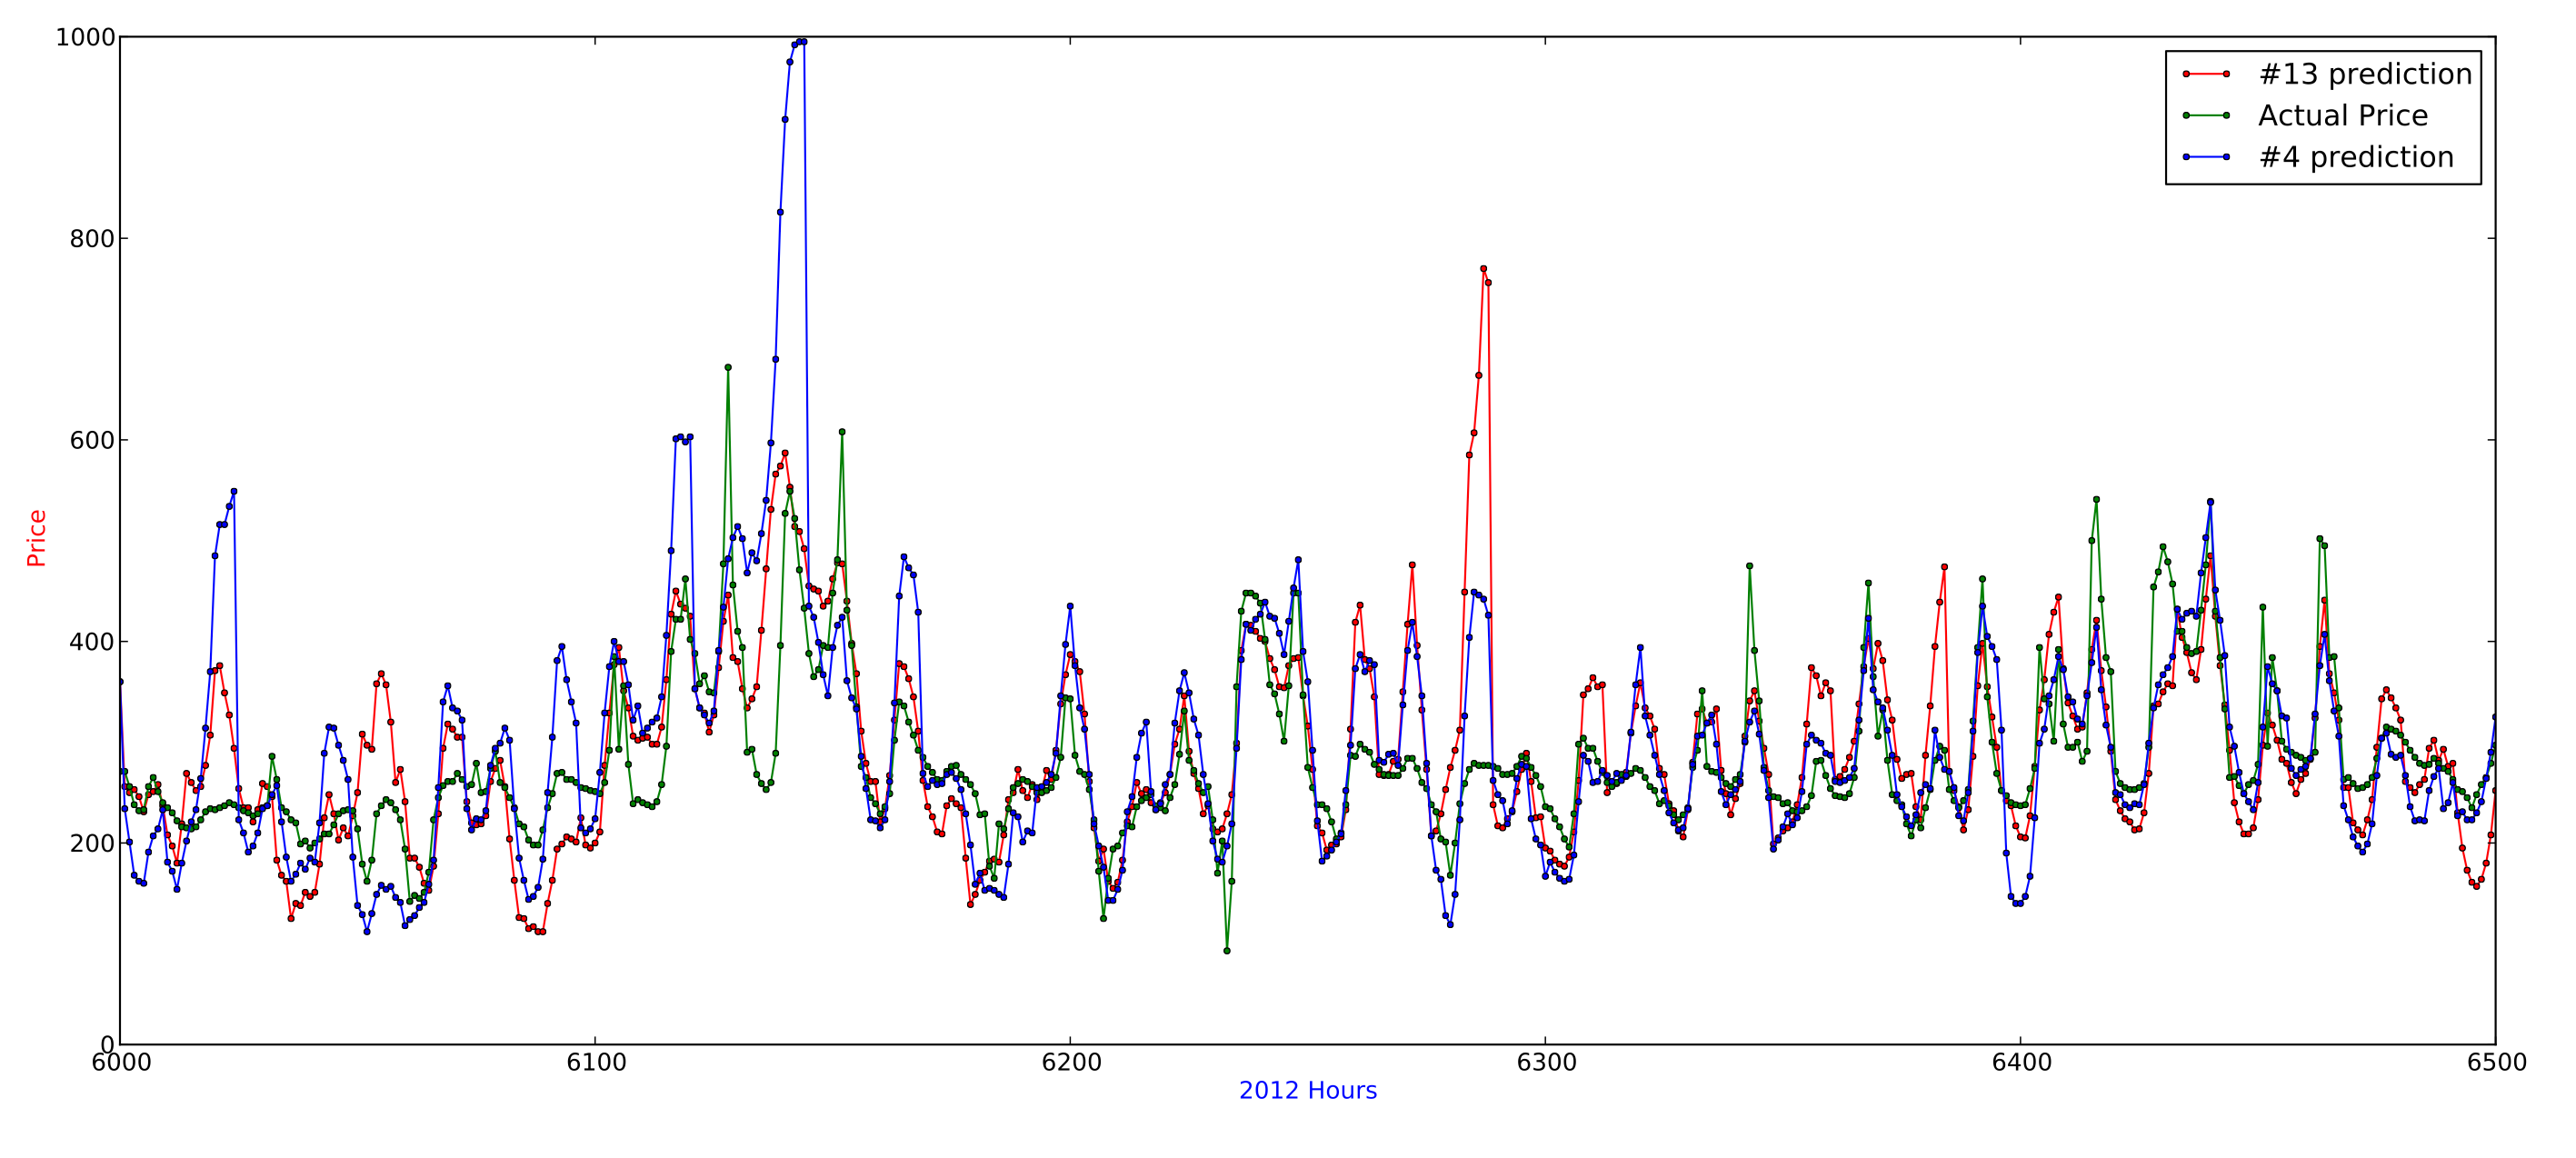
\includegraphics[width=\linewidth]{billeder/PriceExperimentalAnalysis/temperatureComparison.png}
\caption{\#4 forecast from table~\ref{table:Top20Prices} with and without temperature}
\label{fig:temperature_comparison}
\end{figure}

\subsubsection{The Hourly Time of the Day}
The Hourly Time of Day (ToD) is included in every single combination in the top 20. This clearly shows that this input parameter is important for the prediction of the price. This is kind of obvious since what we are predicting is the hourly price. In section~\ref{sec:seasonality}(Figure~\ref{fig:price_per_hour}) we saw that the price varied from 190 to 335 which strengthens the importance of the relationship between time of day and the price. Also the top 7 all have the ToD on matrix form which indicates that this is the best way of representing the ToD. The comparison between \#1 prediction with Time of Day and the one without \#55 we see a difference of 31.85\% and we have done a graph comparison of the two shown in Figure~\ref{fig:dowComparison}. Here we see that the one with ToD (\#1) are better at following the curve compared to the prediction without Time of Day. The prediction without Time of Day seems to follow an average between the high and low spikes instead of following the curve up and down. This makes sense since the ToD is interpreted into what hours have high prices and which have low prices.

\begin{figure}[H]
\centering
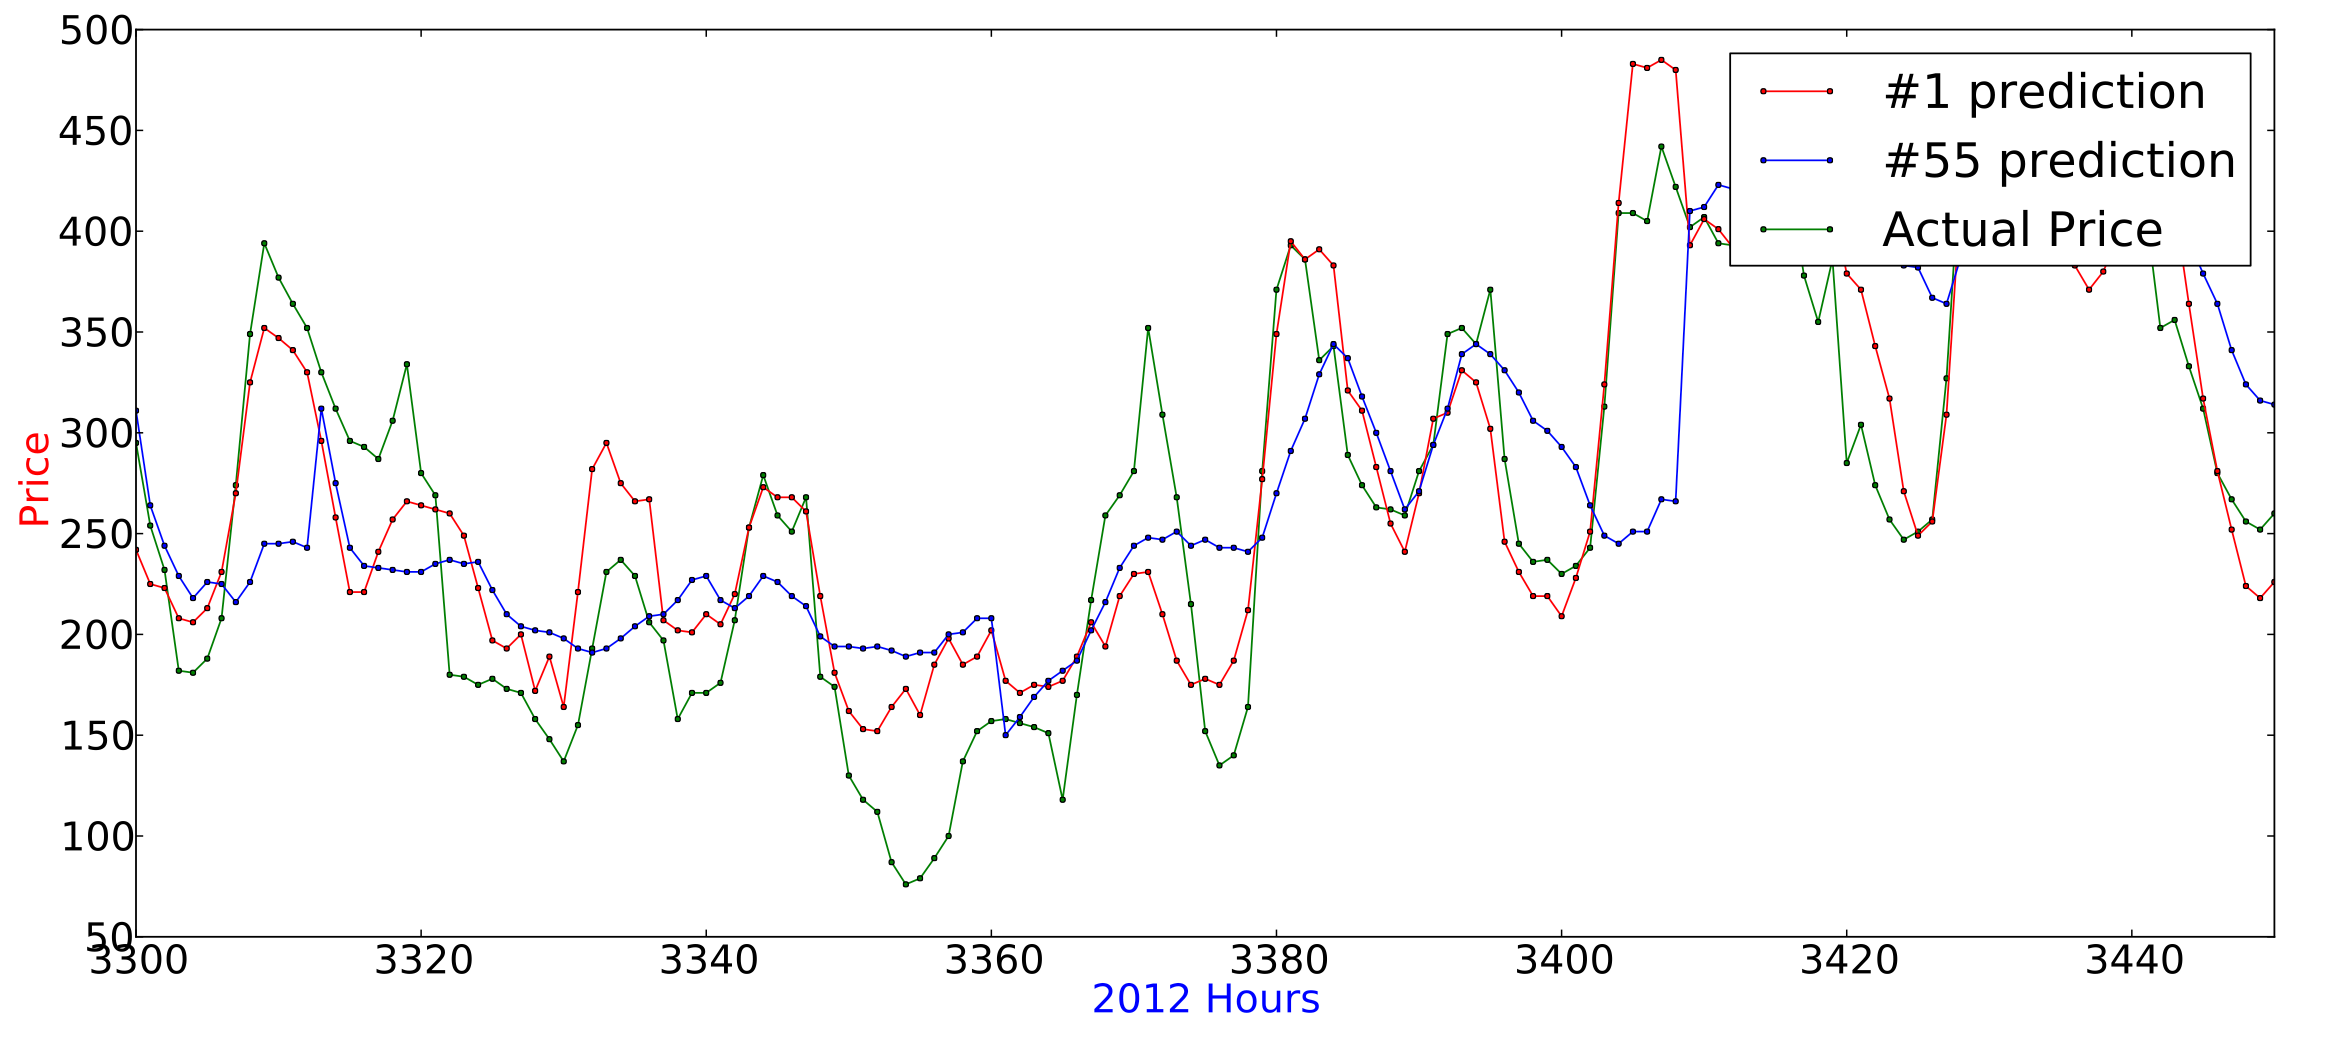
\includegraphics[width=\linewidth]{billeder/PriceExperimentalAnalysis/dowComparison.png}
\caption{\#1 forecast from table~\ref{table:Top20Prices} with and without Time of Day}
\label{fig:dowComparison}
\end{figure}

\subsubsection{The Day of the Week}
Next we have the Day of the Week (DoW) parameter. This parameter is present in 75\% of the 20 best results (8/10 and in 15/20 best combinations). We have to believe that it plays a significant role in the prediction of price. If we look at the analysis of the average price over weekdays in Section~\ref{sec:seasonality} (Figure~\ref{fig:price_over_weekdays}) we see that there is a significant difference in price on the different days. This is especially present in the weekdays compared to the weekend. This parameter is mixed between matrix input and standard input. This might be due to the fact that the biggest difference between days are weekend and weekday thus minimizing the effect of a matrix representation.

\subsubsection{The Season of Year features}
The last two parameters - Month of Year(MoY) and Season of Year (SoY) - are codependent and will be covered together. As mentioned before they cover the same information and we therefore only need one of them at any time. The values are present in 9/10 of the best combinations in Table~\ref{table:Top20Prices}. This is an indicator that the seasonality in the form of MoY and SoY plays a role in predicting the electricity price. Also we saw in the analysis in Section~\ref{sec:seasonality} (Figure~\ref{fig:monthlyAveragePrice} and Section~\ref{fig:seasons}) that the price changes with seasonality and that it especially was more expensive in the winter than the rest of the year.

\subsubsection{Matrix}
The matrix representation in the top 20 is the most common representation of the seasonal inputs (ToD, DoW, MoY and SoY) - with only 3/20 containing no matrix at all. The matrix format was expected to give a better result based on what we discussed in the matrix Section~\ref{sec:Matrix}. The three combinations that does not contain a matrix representation are already present in the top 20 as pure matrix form. This can be the combination of inputs variables that are good since both the matrix form and the non-matrix form are represented in the top 20 best combinations.

In the wind power Experiments section~\ref{sec:windProductionExperiments} we conducted a separate experiment for the matrix analysis. We have done a combined experiment in this section because we had 4 different parameters that can be represented as a matrix thus giving us a lot of different combinations. We also wanted to test all of the different combinations of matrix and non-matrix inputs because a mixed combination might render a better solution e.g. the season of year shifts so rarely it might be a better representation (together with the other parameters) on non-matrix form. Also there might be combinations with the rest of the inputs that work better with the matrix-format than others. 

\subsubsection{Bottom 10 predictions}
\begin{table}[H]
\centering  % used for centering table
\resizebox{\textwidth}{!}{
\begin{tabular}{|c|c|c|c|c|c|c|c|c|c|c|c|c|c|} % centered columns (7 columns)
\hline
{\#} & P & D & WS & T & ToD & DoW & Mo & SoY & \% CD & H1 & H2 & MAE & {\%} Rank \\ [0.5ex] % inserts table 
%heading
\hline 
134 &  \x    & \x    & \x    &       &       & \x\m  & \x\m  &       & 59,8\% &  5  & 0  & 105,70 & 85,05\% \\ \hline
135 &  \x    & \x    &       &       &       & \x\m  &       & \x\m  & 51,4\% &  7  & 0  & 107,85 & 88,81\% \\ \hline
136 &  \x    & \x    &       & \x    & \x    &       & \x    &       & 56,5\% &  5  & 0  & 108,37 & 89,72\% \\ \hline
137 &  \x    & \x    &       & \x    &       &       & \x    &       & 54,4\% &  7  & 0  & 111,14 & 94,57\% \\ \hline
138 &  \x    & \x    &       & \x    &       &       & \x\m  &       & 53,5\% &  8  & 0  & 111,65 & 95,47\% \\ \hline
139 &  \x    & \x    &       & \x    &       & \x\m  & \x\m  &       & 52,9\% &  7  & 0  & 113,56 & 98,81\% \\ \hline
140 &  \x    & \x    &       & \x    &       &       &       & \x    & 52,7\% &  8  & 0  & 115,29 & 101,84\% \\ \hline
141 &  \x    & \x    &       &       &       &       & \x\m  &       & 53,0\% &  11 & 0  & 115,81 & 102,75\% \\ \hline
142 &  \x    & \x    &       & \x    &       & \x\m  &       & \x\m  & 53,0\% &  5  & 0  & 115,83 & 102,78\% \\ \hline
143 &  \x    & \x    &       & \x    &       & \x    & \x    &       & 53,2\% &  6  & 0  & 117,17 & 105,13\% \\ \hline
144 &  \x    & \x    &       &       &       & \x\m  & \x\m  &       & 52,0\% &  7  & 0  & 117,34 & 105,43\% \\ \hline
\end{tabular}
}
\caption{The bottom 10 input combinations for price prediction} % title of Table
\label{table:Bottom10Prices} % is used to refer this table in the text
\end{table}

If we take a look at the bottom 10 input combinations in terms of MAE we see some tendencies as well. We see that wind speed only appears in one of the combinations and so does the Time of Day(And not in the same combination). This further strengthens that these two variables are very important for the price prediction. We talked about matrix form earlier and its impact on the combinations. In the bottom 20 table we see that there is a lot of the combinations that contains variables on matrix form. This is because the wind speed and ToD are some of the most influential parameters thus sending the combinations with these absent to the bottom of the chart. As these combinations also include matrix forms they will occur in the bottom top 20 thus not indicating that matrix form has no effect on the dataset. In the bottom 10 we also see a substantial drop in percentage correct direction(\% CD) which tells us that the trend analysis of the curves also suffers from the worse combinations of inputs. Also this might indicate that wind speed and especially the time of day says something about the price movement.

\subsubsection{Month and season analysis}
The seasonal aspect will be elaborated here based on experiences from the the first experiment for wind power in Section~\ref{sec:windPowerAnalysis}. The experiment showed problems with the seasonal aspect due to a small dataset and the month parameter not reflecting months from the previous year. Even though the same problem is not obvious from the results in the context of electricity pricing we will investigate the benefits from including the seasonal aspect where it identifies the influence of same months from the previous year. We will compared the three months approach with two other training set sizes; 1) include 45 days before the day-ahead prediction and 45 days before and after the day from last year ---  denoted as 3 Months(Last year); 2) including a whole year from the prediction day. The first approach has been run for all combinations so that it can be directly compared to the one used in the previous prediction with only three months of data (denoted 3 Months). The results are compared to the results from Table~\ref{table:Top20Prices} and can be seen in Table~\ref{table:top20comparedTo4months}. 

\begin{table}[H]
\centering  % used for centering table
\resizebox{0.4\textwidth}{!}{
\begin{tabular}{|c|c|c|} % centered columns (7 columns)
	\hline
	{\#} & 3 Months & 3 Months(Last year) \\ [0.5ex] % inserts table 
	%heading
	\hline  
	 1  & 57,12 & 61,70  \\ \hline
	 2  & 58,09 & 68,23  \\ \hline
	 3  & 58,79 & 63,80  \\ \hline
	 4  & 60,14 & 67,82  \\ \hline
	 5  & 62,19 & 74,89  \\ \hline
	 6  & 62,26 & 61,86  \\ \hline
	 7  & 62,84 & 62,62  \\ \hline
	 8  & 63,94 & 72,37  \\ \hline
	 9  & 64,19 & 84,12  \\ \hline
	 10 & 64,72 & 72,29  \\ \hline

	 11 & 65,07 & 79,71  \\ \hline
	 12 & 65,95 & 58,19  \\ \hline
	 13 & 66,55 & 67,31  \\ \hline
	 14 & 67,21 & 74,67  \\ \hline
	 15 & 67,88 & 77,29  \\ \hline
	 16 & 68,21 & 72,45  \\ \hline
	 17 & 68,34 & 72,31  \\ \hline
	 18 & 68,35 & 76,25  \\ \hline
	 19 & 68,43 & 75,10  \\ \hline
	 20 & 68,45 & 75,97  \\ \hline 
\end{tabular}
}
\caption{Top20(3 months) compared to 3 Months(Last year).} % title of Table
\label{table:top20comparedTo4months} % is used to refer this table in the text
\end{table}

We can see in Table~\ref{table:top20comparedTo4months} that the difference between the two datasets are not significant. This also shows in the Appendix~\ref{sec:priceResultAppendix} where the distribution of the MAE over the two datasets are similar. We can conclude that the effect of using last years month in our dataset does not make a significant difference and can be left out. What can be concluded is that the seasonal aspect for electricity price predicting works unexpectedly since t is represented in most of the best results. The seasonal inputs can work unexpectedly to our advantage by gathering information of the past three months so that it in itself contains the seasonal aspect of the small training set. The knowledge of the last three months in the seasonal input can give an advantage when predicting the day-ahead. This is speculation and due to the black box nature the knowledge is hard to extract and therefore we must rely on our intuition and the knowledge from the dataset analysis. To further validate the use of a small dataset we have attempted a test for the best prediction from Table~\ref{table:Top20Prices} and used it with a whole years training set. Table~\ref{table:1YearTrain} shows a significant drop in accuracy due to the increase in dataset. It emphasizes what was concluded for wind power, namely that there is possibility of over-training in too large datasets\cite{1} and that the network takes longer time training on a larger dataset. We can conclude that the smaller dataset of three months are better to use than the full year for electricity prices and wind power (We will elaborate on this in experiment four).  

\begin{table}[H]
\centering  % used for centering table
\begin{tabular}{|c|c|c|c|c|c|c|c|c|c|c|} % centered columns (7 columns)
\hline
P & D & WS & T & ToD & DoW & MoY & SoY & MAE & \% ranking\\ [0.5ex] % inserts table 
\hline
\x    & \x    & \x    & \x    & \x\m  & \x\m  &   & \x\m  & 94.75 & \\ \hline
\end{tabular}
\caption{The top 20 results on training set 3 last months} % title of Table
\label{table:1YearTrain} % is used to refer this table in the text
\end{table}

\subsubsection{Own set vs Unseen set}
Here we present the difference between predicting something that is included in the dataset and something that is new to the dataset. We want to highlight that we always have to use unseen data when benchmarking the Feedforward Neural Network since it simulates the behaviour of the use in practice. In table \ref{table:unseenAndSeen} we see that it performs well on its own training set compared to how it performs on unseen data. The purpose is to generalize beyond the training set because we wish to predict the prices of tomorrow. Predicting on the data that it has based the generalization function upon will make the data fit that generalization better than situations never seen before. In practice we do not encounter the exact same situations again and therefore we must use a testing set that is different from the training set and attempt to predict it. 

\begin{table}[H]
\centering  % used for centering table
\resizebox{0.8\textwidth}{!}{
\begin{tabular}{|c|c|c|c|} % centered columns (7 columns)
	\hline
	{\#} & MAE(Training dataset) & MAE(Unseen dataset) & MAPE(Unseen dataset) \\ [0.5ex] % inserts table 
	%heading
	\hline 
	1  & 20,90 & 57,12 & 21,72\% \\ \hline
	2  & 29,61 & 58,09 & 22,09\% \\ \hline
	3  & 25,49 & 58,79 & 22,35\% \\ \hline
	4  & 18,94 & 60,14 & 22,87\% \\ \hline
	5  & 31,10 & 62,19 & 23,65\% \\ \hline
	6  & 22,97 & 62,26 & 23,67\% \\ \hline
	7  & 20,64 & 62,84 & 23,89\% \\ \hline
	8  & 23,87 & 63,94 & 24,31\% \\ \hline
	9  & 17,76 & 64,19 & 24,41\% \\ \hline
	10 & 19,79 & 64,72 & 24,61\% \\ \hline
	11 & 20,85 & 65,07 & 24,74\% \\ \hline
	12 & 25,71 & 65,95 & 25,08\% \\ \hline
	13 & 30,02 & 66,55 & 25,30\% \\ \hline
	14 & 31,32 & 67,21 & 25,56\% \\ \hline
	15 & 31,80 & 67,88 & 25,81\% \\ \hline
	16 & 23,11 & 68,21 & 25,94\% \\ \hline
	17 & 30,39 & 68,34 & 25,98\% \\ \hline
	18 & 40,54 & 68,35 & 25,99\% \\ \hline
	19 & 29,40 & 68,43 & 26,02\% \\ \hline
	20 & 34,38 & 68,45 & 26,03\% \\ \hline
	\end{tabular}
}
\caption{The MAE of the training dataset compared to the MAE of the unseen dataset.} % title of Table
\label{table:unseenAndSeen} % is used to refer this table in the text
\end{table}

\subsubsection{Conclusion}
In this experiment we saw the following:
\begin{itemize}
	\item The wind speed clearly was a factor that influenced how well we were able to predict the price. The wind speed was in the best 70/144 combinations. We also saw that the wind speed helped the ANN to overshoot fewer times. The wind speed showed a greater impact on the price prediction than we first thought. With an improvement of 37.55\% it is concluded to be very important for our algorithm to make good predictions.
	\item The temperature showed no real improvement but neither did it deteriorate the result. This was expected since there was nearly no correlation between the price and temperature see section~\ref{sec:ElectricityPriceAnalysis}. It could neither substitute demand as it was seen for wind power.
	\item The Hourly Time of Day shows an improvement on the predictions. In the best half of the results we had 55 that included ToD. This result directly reflects what we anticipated. We also saw that the ToD allowed the ANN to make a better curve fit and helped the predictions to follow the curves all the way up and down instead of following an average between the top and bottom of the curve.
	\item The Day of the Week seemed to have a positive effect on the predictions. Here it was not clear whether the matrix form was the best choice or the standard single input was the best. This stems from the fact that the biggest price difference in weekdays are between the regular weekdays and the weekend.
	\item The Month of the Year and the Seasons of the Year seems to either have no effect or a small effect on the predictions. We discussed how the main purpose of these two input parameters was defeated because of the size of our dataset. They do nevertheless show up in most of the top 20 values. This shows us that they have a positive effect or at worst no effect at all.
	\item Matrix representation seems to be the best choice in almost all the cases. The matrix format is not by default an improvement but has to be evaluated with the rest of the input parameters to see if matrix is better. One of the cases where it might be better without it is the weekdays; because of the aforementioned price distribution over weekdays.
\end{itemize}

\newpage
\subsection{Experiment Two - Data Manipulation}
\label{sec:priceExperimentTwo}
As described in section~\ref{sec:Trimming} trimming is a solution to extreme outliers and a way to streamline your data; thus making it easier for neural networks to predict. The art is to get a good balance between how much of the dataset you remove and how much of an accuracy boost your predictions will get. If you trim parts of the dataset that is actually common data it will get impossible to predict a very high price since the network never sees those values.

\subsubsection{Variables}
Experiment two is based on a dataset consisting of the last three months averaging to 2189 hours. We use 200 epochs for each training iteration.

In this experiment our variables are the grade of trimming we conduct on the training set. We trim from 1\% to 5\% in the lowest and highest part of the dataset thus totalling to 2\% to 10\% of dataset has been removed.

\subsubsection{Hypothesis}
This experiment is conducted to show the effect of trimming on a dataset. By removing the most extreme outliers we expect the predictions to stabilize since the randomness of the extreme outliers have been removed. This should result in a better overall MAE and a better curve fit.

\begin{figure}[H]
\centering
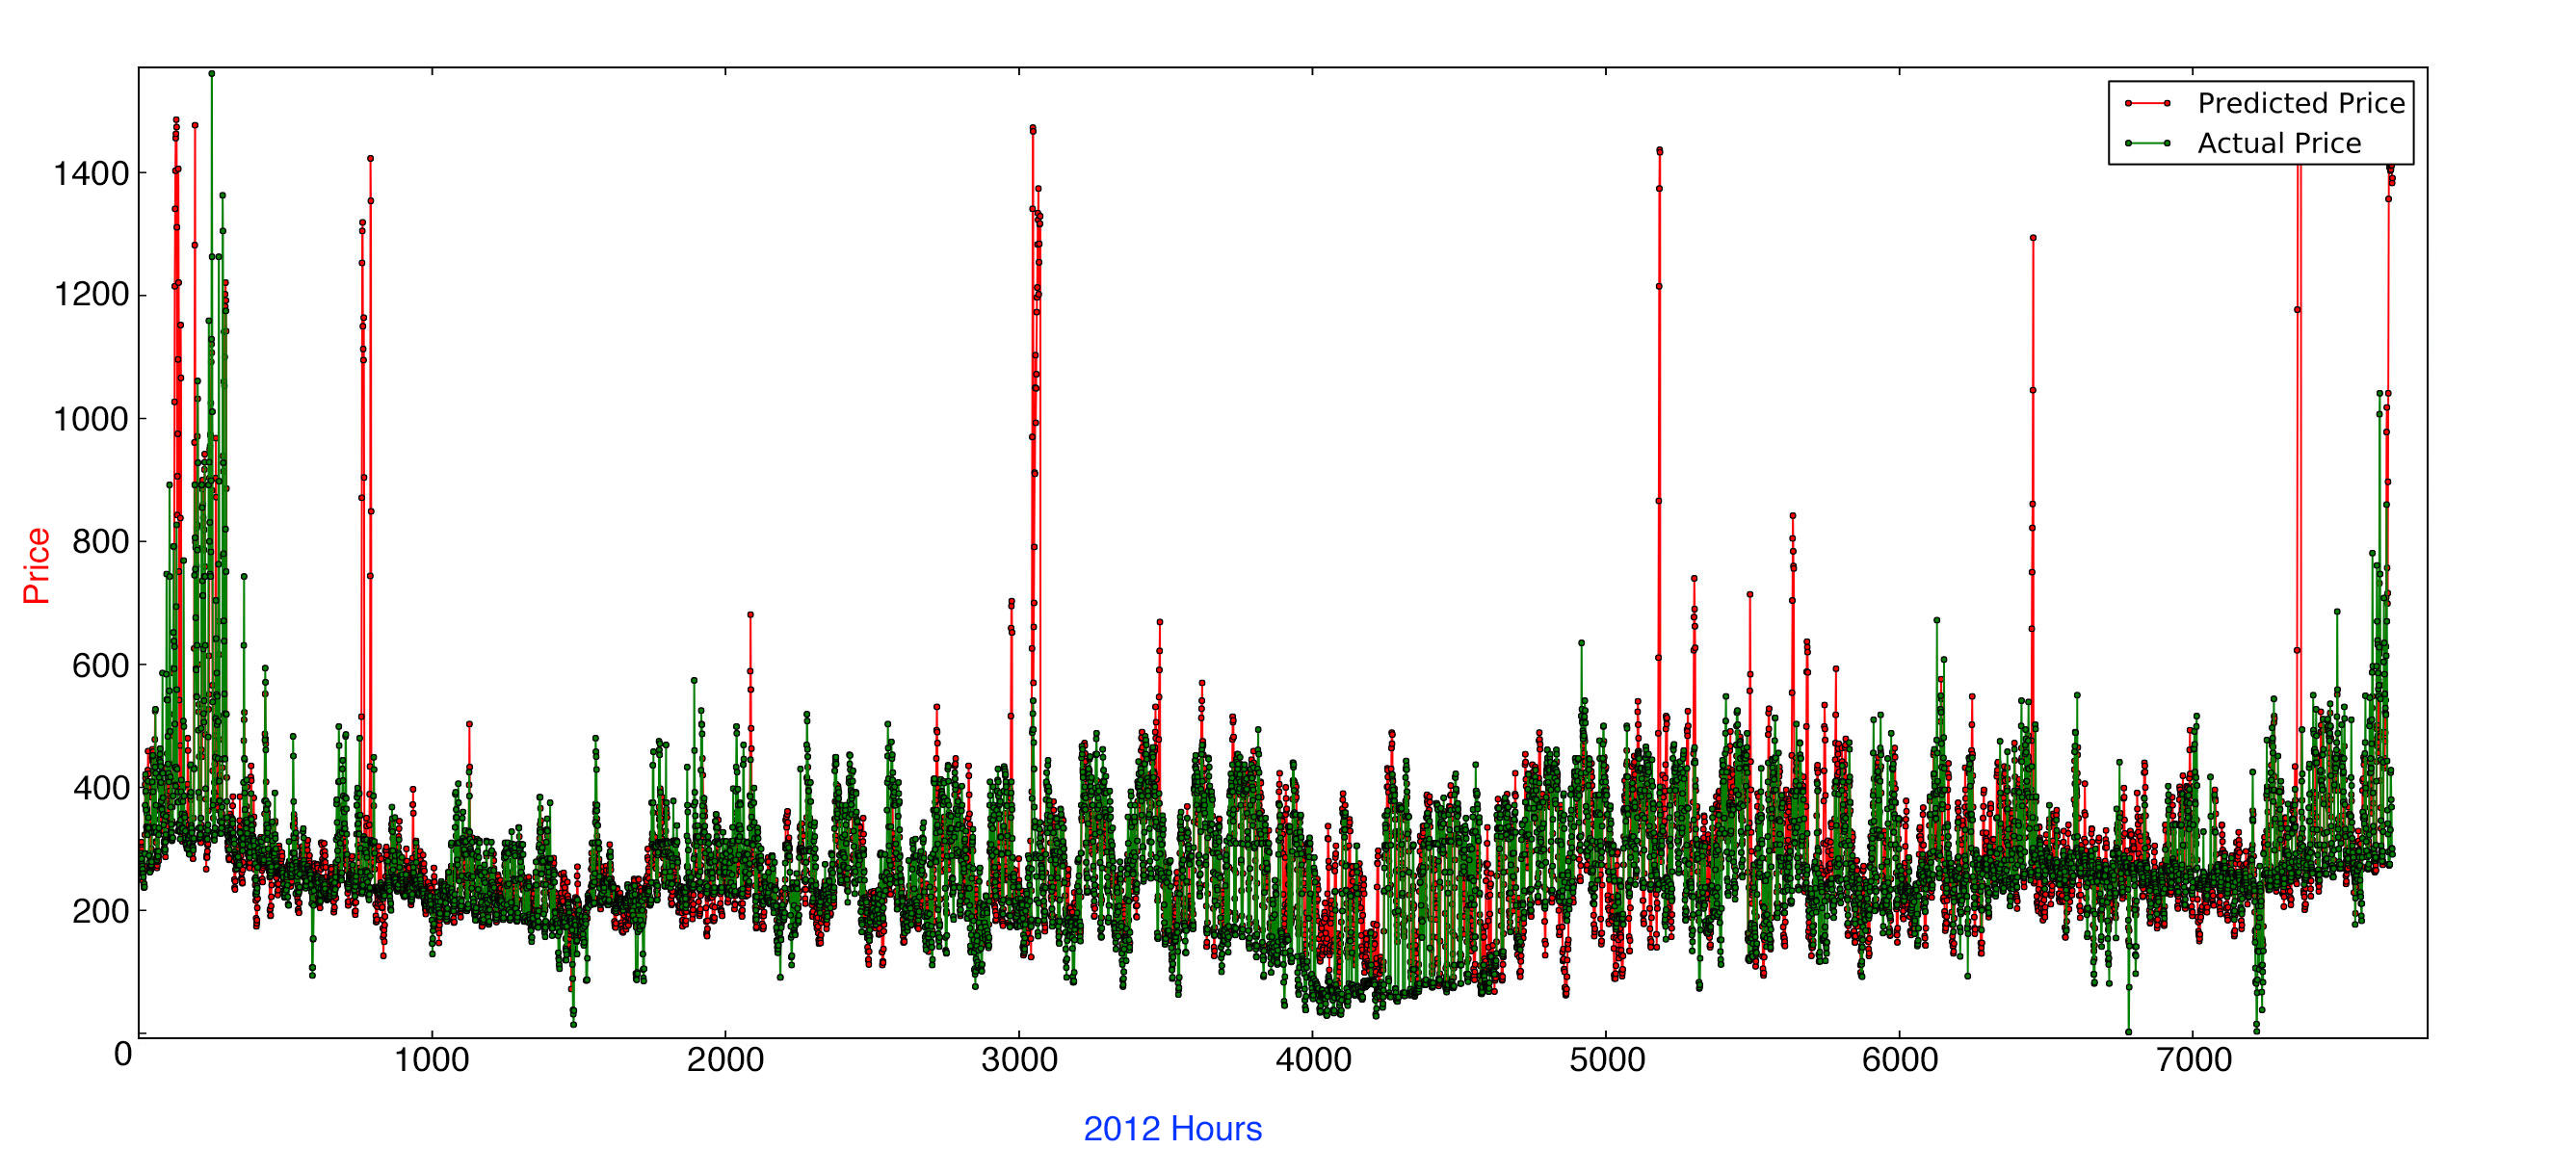
\includegraphics[width=\linewidth]{billeder/PriceExperimentalAnalysis/NoTrimming.png}
\caption{The \#1 forecast from experiment one with no trimming of the dataset}
\label{fig:NoTrim}
\end{figure}

\subsubsection{Results}
As we can see in Figure~\ref{fig:NoTrim} (where no trimming was applied) the predicted values some times goes way out of line and hits the very maximum (about 1500) also when the actual value is nothing near that. This is due to the seldom occurrence of these high prices that the network is never able to get a full connection between these prices and the input parameters. Another reason for this to happen is that it is extremely hard to predict sudden and very high fluctuations in price; thus removing these will not give us a performance hit, since we would not be able to predict them and they would just add the possibility of errors in the rest of the predictions.

If we take a look at the same dataset but this time with a 1\% high and low trim (2\% in total) in Figure~\ref{fig:1PTrim}; we clearly see that the actual prices in the beginning are not spiking as heavily as they did in Figure~\ref{fig:NoTrim}. This of course prevents us from predicting these high spikes but if we take a look at the rest of the set we see that the 5 faulty spikes are gone as well. This shows the trade-off between being able to predict the outliers and the errors they introduce.

\begin{figure}[H]
\centering
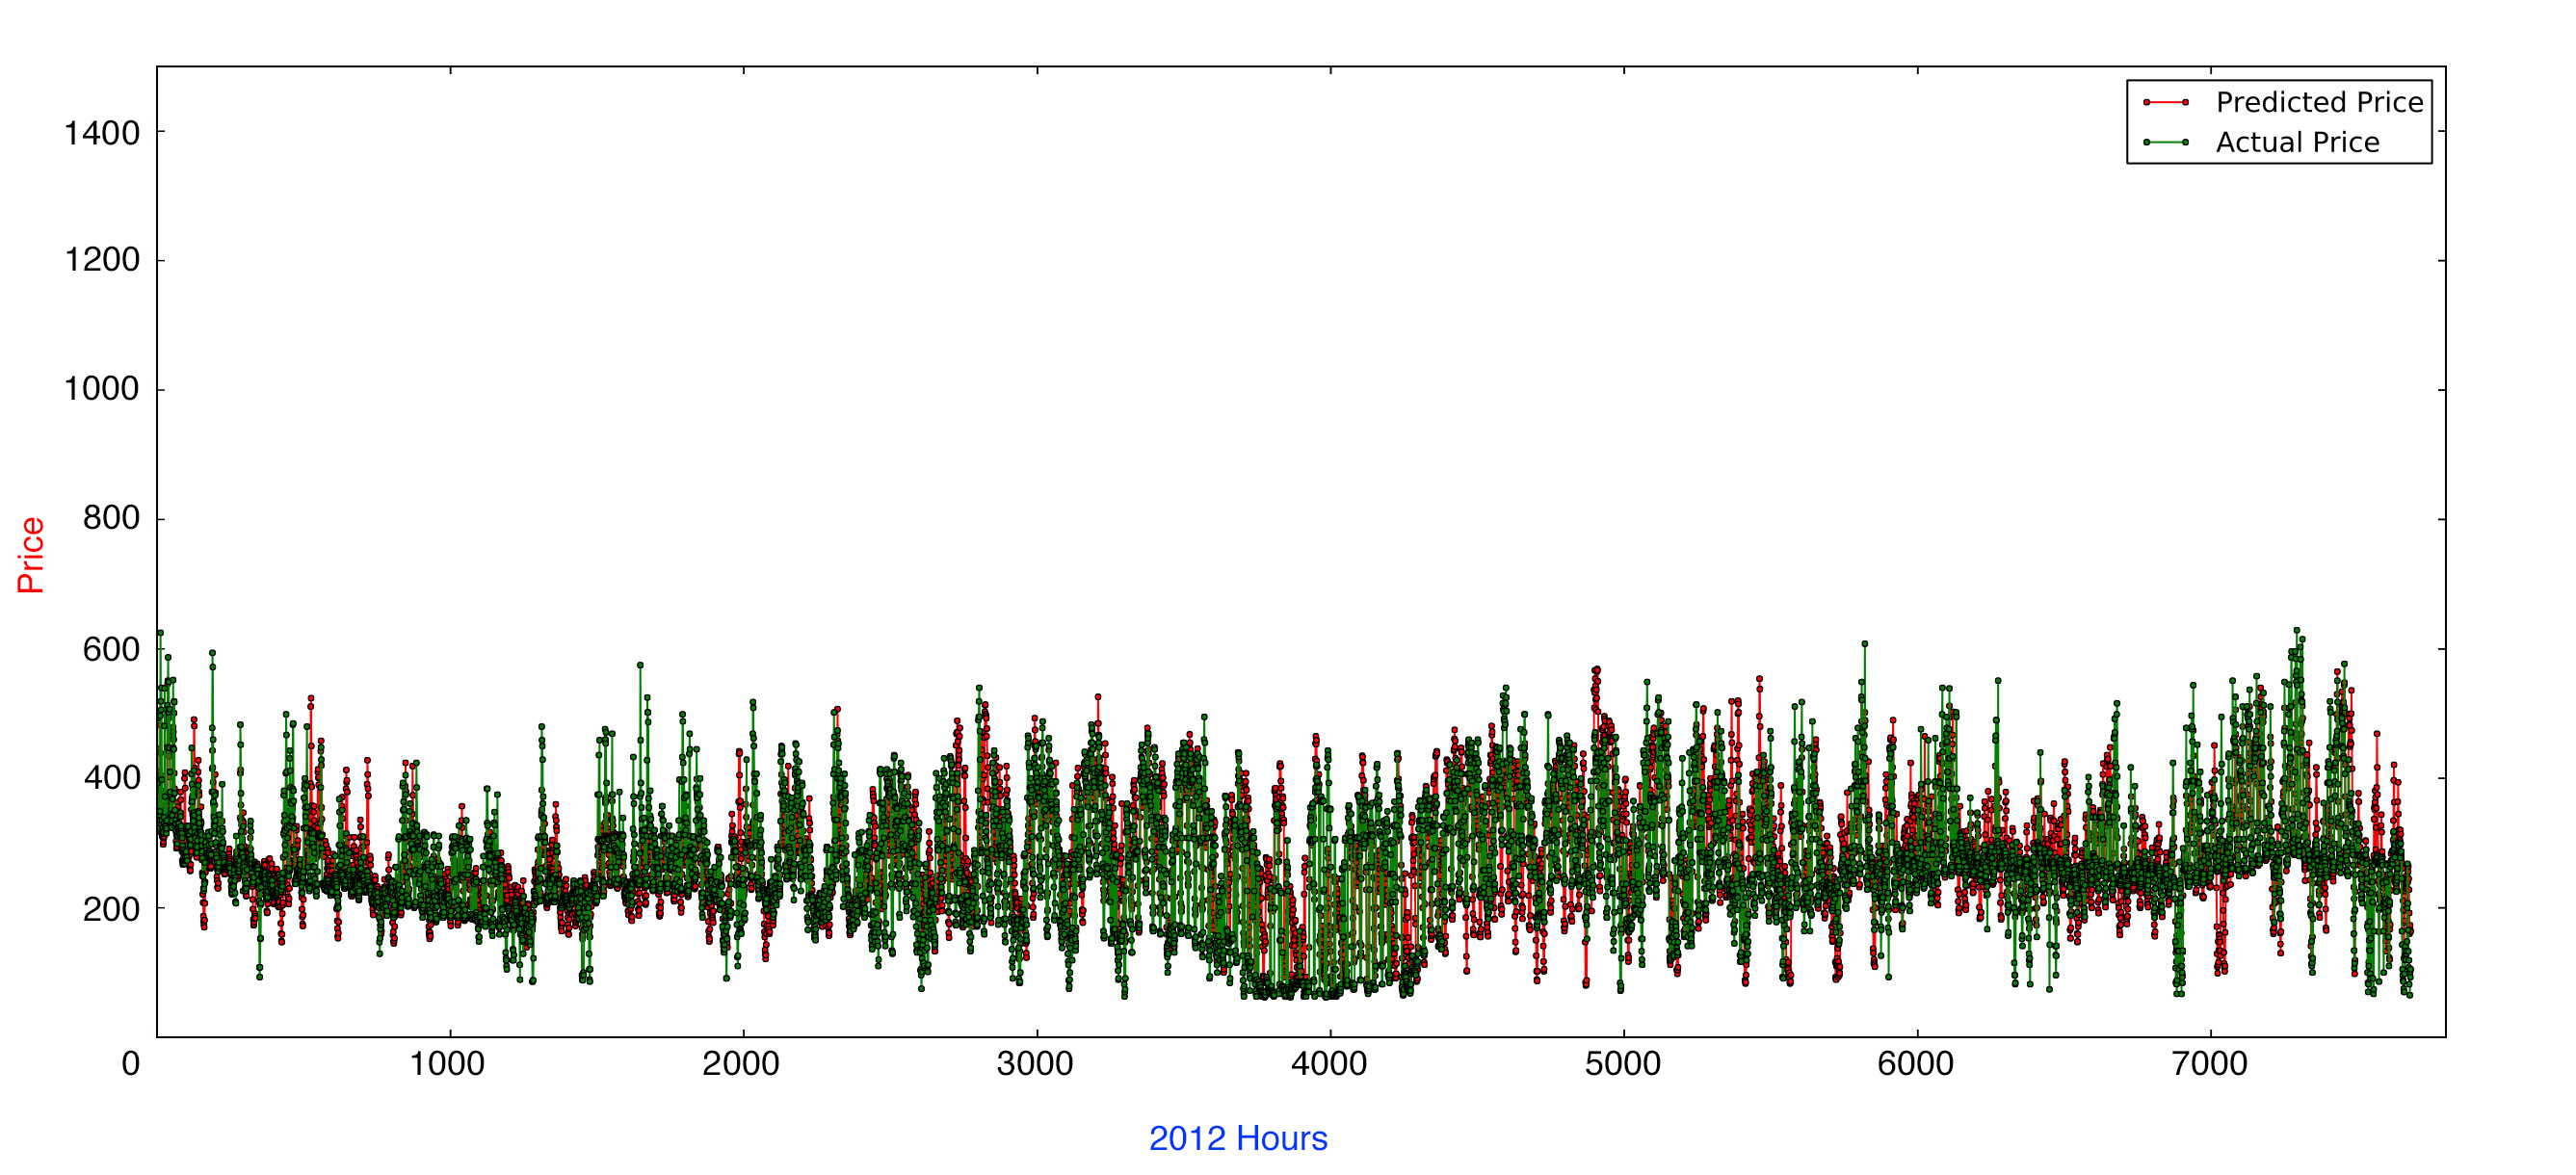
\includegraphics[width=\linewidth]{billeder/PriceExperimentalAnalysis/1PTrim.png}
\caption{The \#1 forecast from experiment one with 1\% trimming in both ends of the dataset}
\label{fig:1PTrim}
\end{figure}

In Figure~\ref{fig:AllTrims} we see the dataset from figure~\ref{fig:1PTrim} with 1\% trim. The lines shows how much would be cut of if we applied 2\%(Purple), 3\%(Red), 4\%(Black) and 5\%(Blue) trimming. Here we clearly see that it is removing data - that is part of the norm - from the set. With every percent we go up we remove 363 entries so at 5\% trim (top and bottom) we will be removing 1815 entries from our dataset. This will result in us never being able to predict values higher or lower than the bars. We are of course not interested in that as most of the values we trim from 2\% and up are part of a more normalized dataset. The improvements we see from 1\% trim to 5\% trim is 12.97\% but if it implies that the network cannot predict 1815 hours of a year then it not worth using when simulating a whole year prediction.

\begin{figure}[H]
\centering
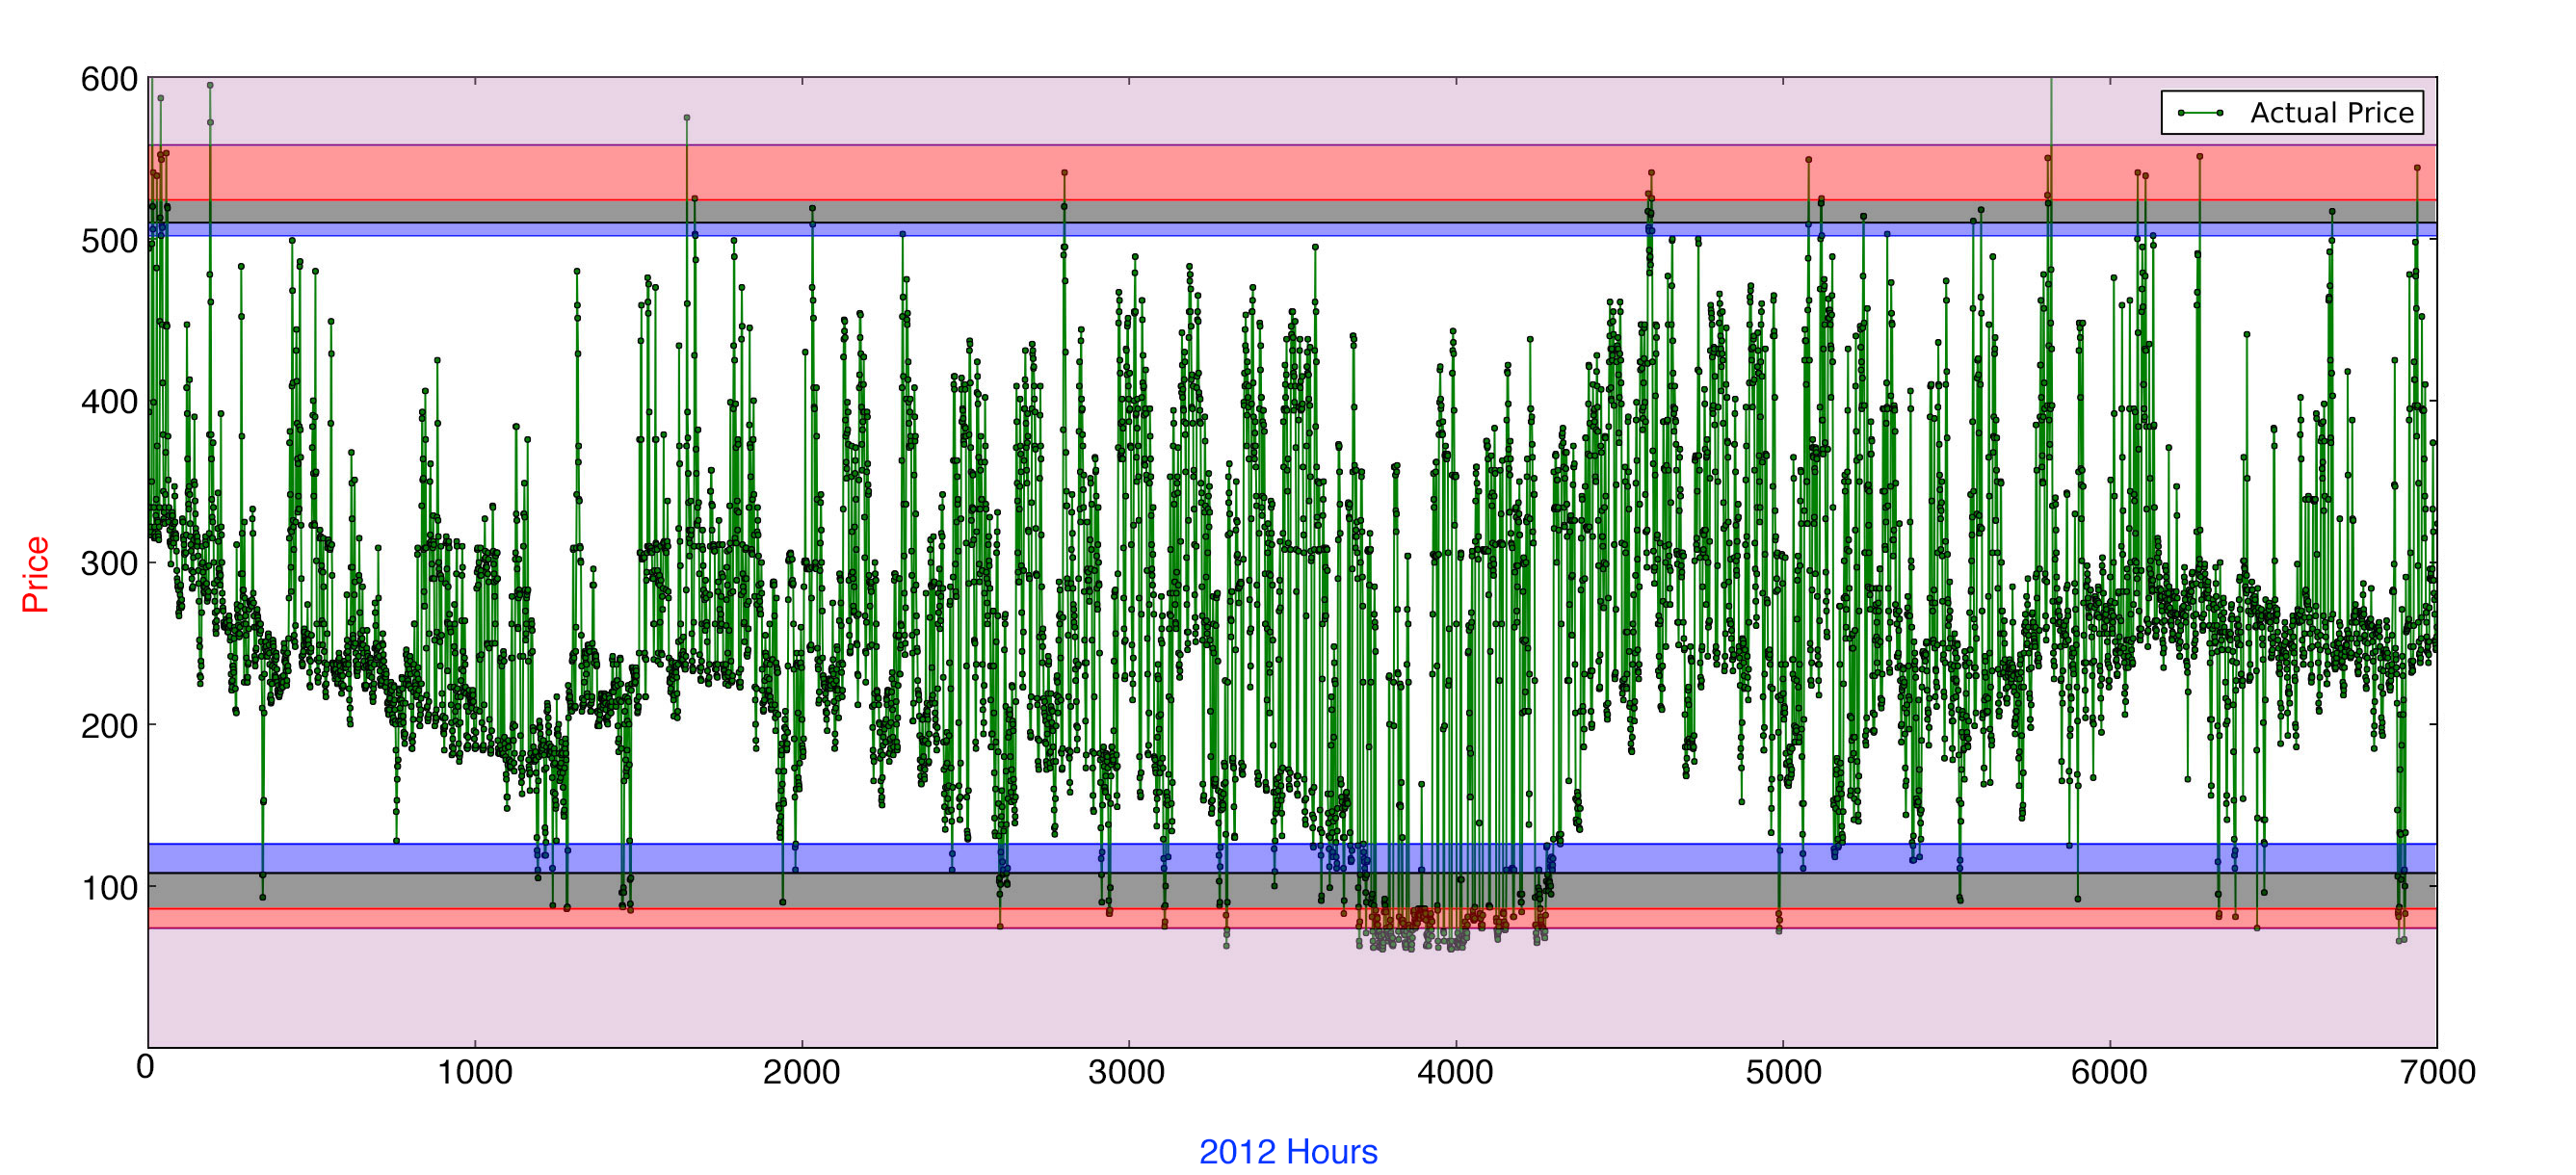
\includegraphics[width=\linewidth]{billeder/PriceExperimentalAnalysis/restOfTrims.png}
\caption{The \#1 forecast from experiment one with 2\%(Purple), 3\%(Red), 4\%(Black) and 5\%(Blue) trimming in both ends of the dataset}
\label{fig:AllTrims}
\end{figure}

In Figure \ref{fig:AllTrims200Hours} we have shown all of the trims on 200 hours. Here we can see that many of the spikes are limited to few hours. We can also see that the green box represents how much of the price interval the top 1\% of the dataset represents.

\begin{figure}[H]
\centering
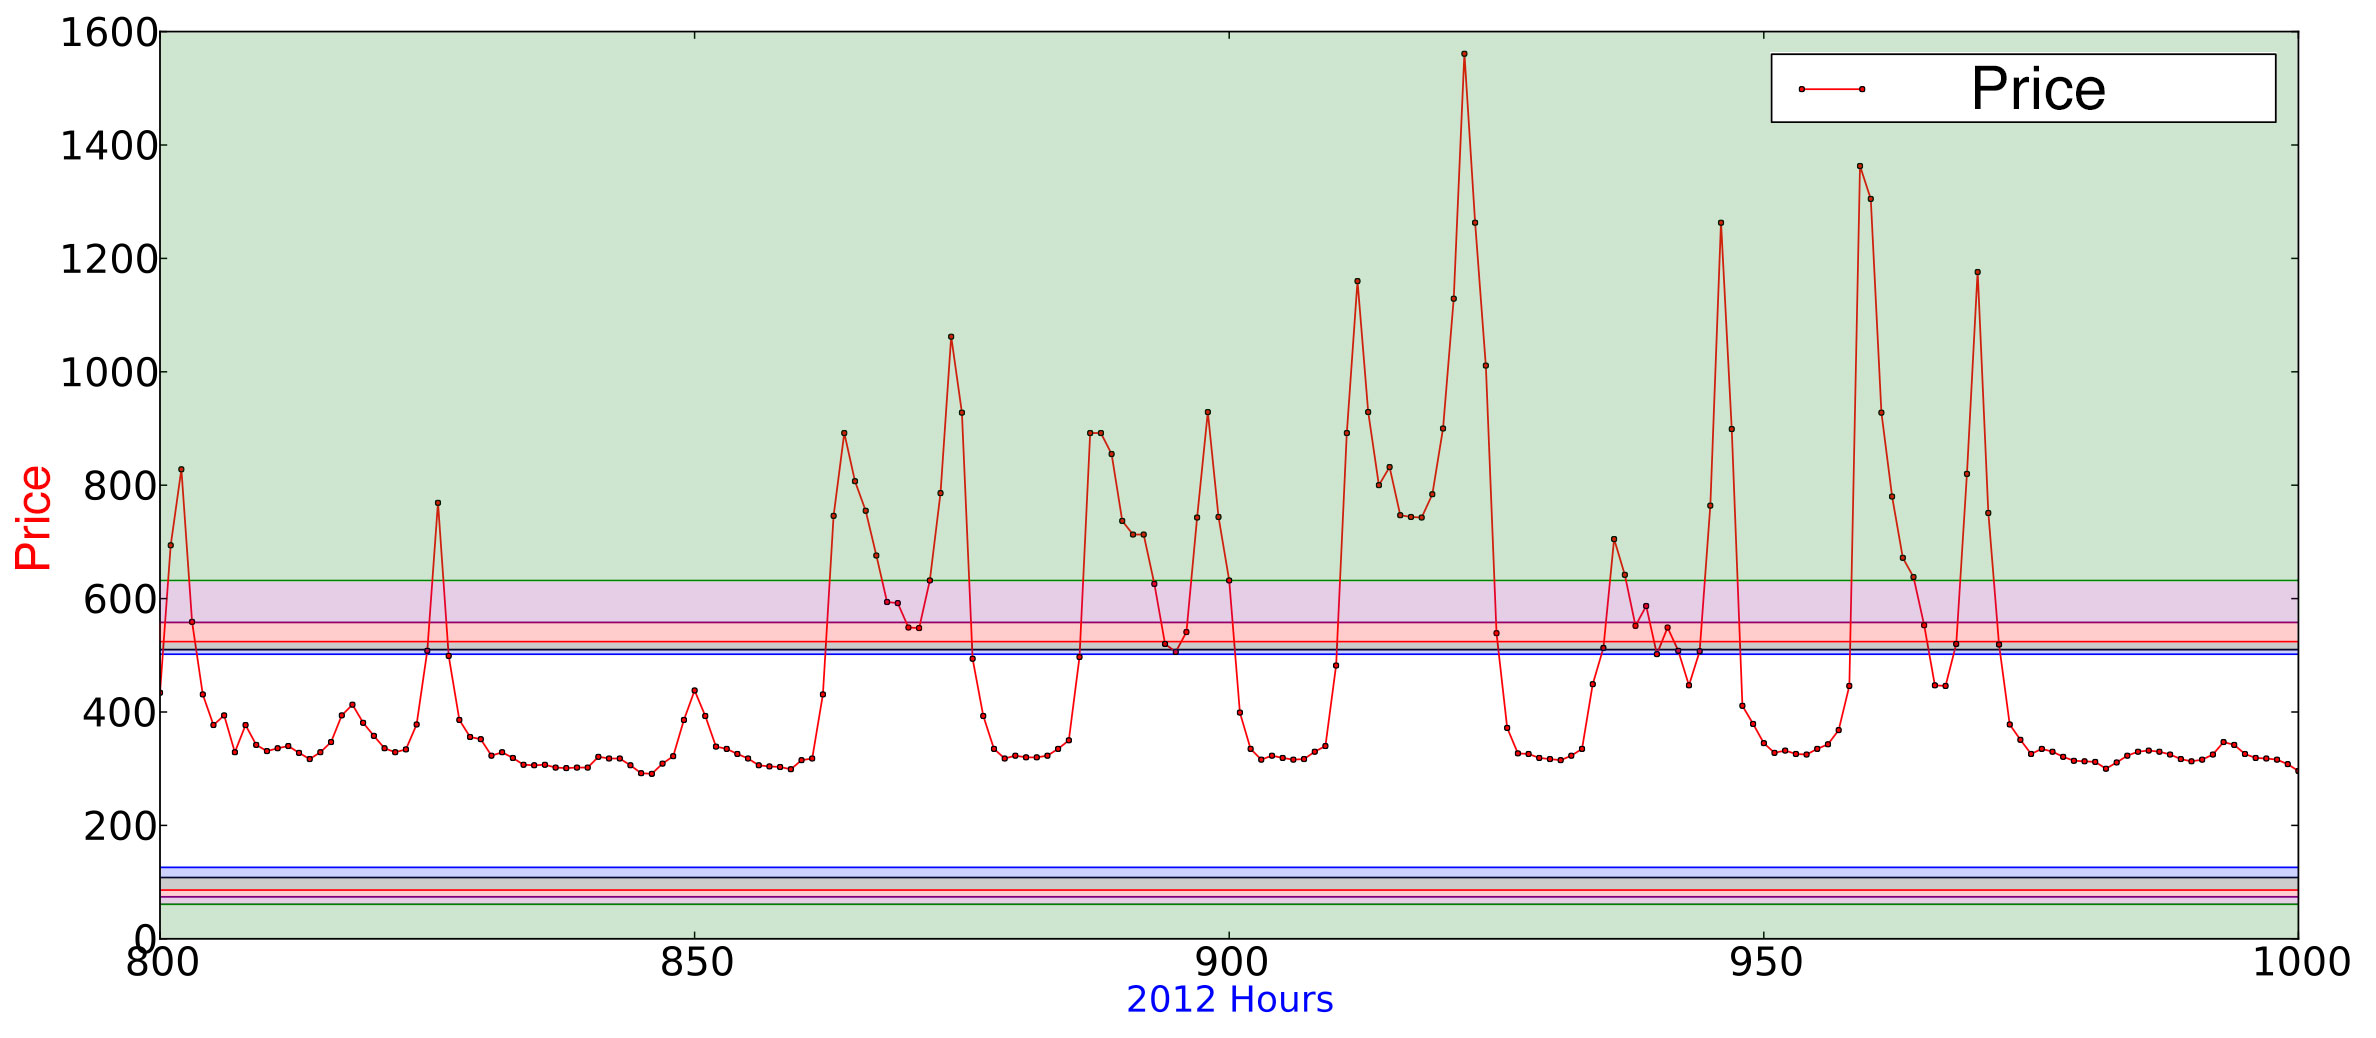
\includegraphics[width=\linewidth]{billeder/PriceExperimentalAnalysis/200hoursTrimming.jpg}
\caption{The \#1 forecast from experiment one with 1\%(Green), 2\%(Purple), 3\%(Red), 4\%(Black) and 5\%(Blue) trimming in both ends of the dataset. This is a segment of 200 hours.}
\label{fig:AllTrims200Hours}
\end{figure}

\begin{table}[H]
\centering  % used for centering table
\resizebox{0.6\textwidth}{!}{
	\begin{tabular}{|c|c|c|c|c|c|} % centered columns (7 columns)
	\hline
	\# & \% Trim & \% CD & MAPE & MAE & \% Rank\\ [0.5ex] % inserts table 
	\hline                  % inserts single horizontal line
	1  & 5 & 69,7\% & 15,09\% & 40,42 & - \\ \hline
	2  & 4 & 70,0\% & 15,21\% & 40,74 & 0,8\% \\ \hline
	3  & 2 & 70,5\% & 16,15\% & 43,25 & 7,0\% \\ \hline
	4  & 3 & 69,5\% & 17,00\% & 45,51 & 12,59\% \\ \hline
	5  & 1 & 69,2\% & 17,70\% & 47,41 & 17,29\% \\ \hline
	\end{tabular}
}
\caption{Trims} % title of Table
\label{table:Top10Trimming} % is used to refer this table in the text
\end{table}

\subsubsection{Conclusion}
In this experiment we saw how trimming can positively affect the predictions. We also discussed the trade-offs in the trimming procedure as we lowered the possible outcomes of our predictions. This is a balance between improvement and the amount of prices we will not be able to predict. The 1\% trim showed us an improvement of 20.48\% and removed some extreme failed predictions where the ANN would overshoot the target by 800+. We also learned that higher trimming rates did not really improve the results very much thus making it easy for us to decide on a trimming rate of 1\%.

\newpage
\subsection{Experiment Three - Calculated inputs}
\label{sec:priceExperimentThree}
This experiment has been conducted to test the different calculated inputs that we described in Section~\ref{sec:usingStatisticalInput}. This includes slope calculation, skewness, historical volatility and scatter. We took the three best results from experiment one and ran every combination of the calculated inputs on the best results. The experiment was conducted on the 1\% trimmed version of the 3 best results from experiment one - due to the improvements seen in experiment two where the benefits of trimming was established. Also we have done a test on the most basic dataset we had available: Price and demand with no trimming. This was done to validate the impact of the different strategies before applying any other factors to the prediction. The interesting part is to see how much the strategies can make up for the missing meteorological factors that have shown to be of importance to the prediction. It will give an indication of the calculated inputs potential. We also reconstructed the experiment in \cite{singhal2011electricity} to test their setup which is what is referring to as scatter.

\subsubsection{Hypothesis}
In this experiment we applied different calculated inputs to the Feedforward Neural Network. This was done to elaborate on the prior trend when trying to predict the next 24 hours. This experiment is expected to show an improvement in the curve fitting thus giving us a better MAE.

We conducted an experiment to test the effect of these strategies on a dataset containing demand and last know price with and without trim where we expect these predictions to improve a great deal with strategies applied.

\subsubsection{Variables}
In this experiment we had 4 variables that we tested:
\begin{itemize}
	\item Slope calculation (Slope)
	\item Skewness (Skew)
	\item EWMA - Historical Volatility (EWMA)
	\item Scatter (Scatter)
\end{itemize}

The setup of the different strategies have been tested on the best result from experiment one. The scatter strategy is included to let the Feedforward Neural Network train and find these connections by itself. The rest of the calculated inputs are preprocessed beforehand and directly says something about the graph behavior.

\subsubsection{EWMA - Historical Volatility}
The EWMA is used to calculate the volatility of the curve. The electricity price is highly volatile and therefore we anticipate that knowledge about the historical volatility will help the predictions. In the EWMA we have a smoothing factor which indicates how sensitive the strategy will be towards fluctuations in the curve. A lower smoothing factor will allow for more rapid changes and vice versa. In table~\ref{table:SmoothingFactorTest} we see that the best result is a smoothing factor of 0.9 and a stack size of 16. The stack size denotes how many historical prices should be included in the calculations of the historical volatility.

\begin{table}[H]
\centering  % used for centering table
\resizebox{0.7\textwidth}{!}{
	\begin{tabular}{|c|c|c|c|c|c|c|} % centered columns (7 columns)
	\hline
	\# & Stack size & Smoothing factor & \% CD & MAPE & MAE & \% Rank \\ [0.5ex] % inserts table 
	\hline                   % inserts single horizontal line
	1  & 16 & 0,9 & 67,1\% & 17,56\% & 45,96 & - \\ \hline
	2  & 12 & 0,1 & 66,7\% & 17,63\% & 46,13 & 0,38\% \\ \hline
	3  & 20 & 0,9 & 66,9\% & 17,76\% & 46,47 & 1,11\% \\ \hline
	4  & 8  & 0,9 & 67,1\% & 17,79\% & 46,55 & 1,28\% \\ \hline
	5  & 20 & 0,5 & 66,7\% & 17,79\% & 46,56 & 1,31\% \\ \hline
	6  & 24 & 0,4 & 67,3\% & 17,80\% & 46,58 & 1,36\% \\ \hline
	7  & 20 & 0,7 & 66,4\% & 17,80\% & 46,59 & 1,37\% \\ \hline
	8  & 12 & 0,9 & 67,9\% & 17,81\% & 46,61 & 1,41\% \\ \hline
	9  & 24 & 0,8 & 67,8\% & 17,88\% & 46,78 & 1,79\% \\ \hline
	10 & 24 & 0,5 & 67,1\% & 17,91\% & 46,88 & 2,0\% \\ \hline
	\end{tabular}
}
\caption{Smoothing factor test} % title of Table
\label{table:SmoothingFactorTest} % is used to refer this table in the text
\end{table}

\subsubsection{Skewness}
The skewness denotes whether an observation falls to the left or the right of the median as described in Section~\ref{sec:skewness}. This is used to determine in what direction the graph is currently moving thus giving us information about the trend. We experimented with how many historical prices we had to include in the calculation of the skewness and ended up with 2 being the best even though they are very close.

\begin{table}[H]
\centering  % used for centering table
\resizebox{0.7\textwidth}{!}{
	\begin{tabular}{|c|c|c|c|c|c|} % centered columns (7 columns)
	\hline
	\# & Hours & \% CD & MAPE & MAE & \% Rank \\ [0.5ex] % inserts table 
	\hline                  % inserts single horizontal line
	1  & 2  & 69,1\% & 17,12\% & 44,81 & - \\ \hline
	2  & 8  & 68,7\% & 17,26\% & 45,16 & 0,77\% \\ \hline
	3  & 4  & 69,5\% & 17,28\% & 45,21 & 0,9\% \\ \hline
	4  & 20 & 68,8\% & 17,39\% & 45,50 & 1,53\% \\ \hline
	5  & 24 & 69,3\% & 17,53\% & 45,87 & 2,37\% \\ \hline
	6  & 6  & 68,8\% & 17,58\% & 46,02 & 2,69\% \\ \hline
	7  & 16 & 68,5\% & 17,79\% & 46,55 & 3,88\% \\ \hline
	8  & 12 & 68,6\% & 17,81\% & 46,61 & 4,01\% \\ \hline
	\end{tabular}
}
\caption{Number of historical prices to include in the skewness calculation} % title of Table
\label{table:SkewnessTest} % is used to refer this table in the text
\end{table}

\subsubsection{Slope calculation}
The slope calculation is conducted to tell us something about the gradient of the current curve as described in Section~\ref{sec:curveAnalysis}. We examine here how many historical prices should be included in the curve gradient analysis to say something about what direction (up, down or steady) the curve is heading. The test shows us that a stack size of 12 prices is the best but again they are not differing much.

\begin{table}[H]
\centering  % used for centering table
\resizebox{0.7\textwidth}{!}{
	\begin{tabular}{|c|c|c|c|c|c|} % centered columns (7 columns)
	\hline
	\# & Hours & \% CD & MAPE & MAE & \% Rank \\ [0.5ex] % inserts table 
	\hline                  % inserts single horizontal line
	1  & 12  & 67,3\% & 17,16\% & 44,91 & - \\ \hline
	2  & 2   & 67,9\% & 17,49\% & 45,76 & 1,88\% \\ \hline
	3  & 16  & 67,4\% & 17,56\% & 45,96 & 2,32\% \\ \hline
	4  & 20  & 67,5\% & 17,69\% & 46,29 & 3,07\% \\ \hline
	5  & 4   & 67,0\% & 17,74\% & 46,43 & 3,38\% \\ \hline
	6  & 6   & 68,1\% & 17,79\% & 46,57 & 3,68\% \\ \hline
	7  & 24  & 67,0\% & 18,06\% & 47,26 & 5,22\% \\ \hline
	8  & 8   & 67,9\% & 18,25\% & 47,76 & 6,33\% \\ \hline
	\end{tabular}
}
\caption{Slope calculation stack size} % title of Table
\label{table:CurveTest} % is used to refer this table in the text
\end{table}

\subsubsection{Results}
We ran three experiments reflecting the top 3 results from experiment one. Before the results of the experiments we list the input variable combination that we use the strategies on. 

\noindent Variables: Price, Demand, Wind Speed, Temperature, Time of Day (Matrix), Day of Week (Matrix) and Season of Year (Matrix)
\begin{table}[H]
\centering  % used for centering table
\resizebox{0.8\textwidth}{!}{
	\begin{tabular}{|c|c|c|c|c|c|c|c|c|} 
	\hline
	\# & Curve & Skew & EWMA & Scatter & \% CD & MAPE & MAE & \% Rank\\ [0.5ex] % inserts table 
	\hline                  % inserts single horizontal line
	1  &        & \x    & \x    &       & 66,4\% &  17,33\% & 45,35 & - \\ \hline
	2  &  \x    & \x    & \x    &       & 66,0\% &  17,49\% & 45,76 & 0,91\% \\ \hline
	3  &  \x    &       &       & \x    & 68,4\% &  17,51\% & 45,83 & 1,06\% \\ \hline
	4  &  \x    &       &       &       & 69,7\% &  17,62\% & 46,10 & 1,66\% \\ \hline
	5  &  \x    & \x    &       &       & 68,9\% &  17,73\% & 46,40 & 2,32\% \\ \hline
	6  &  \x    &       & \x    &       & 65,8\% &  17,76\% & 46,47 & 2,48\% \\ \hline
	7  &        & \x    &       &       & 69,4\% &  17,78\% & 46,53 & 2,6\% \\ \hline
	8  &        &       & \x    &       & 66,4\% &  17,78\% & 46,53 & 2,61\% \\ \hline
	9  &        &       & \x    & \x    & 66,1\% &  17,85\% & 46,72 & 3,03\% \\ \hline
	10 &        &       &       & \x    & 68,5\% &  17,91\% & 46,88 & 3,38\% \\ \hline
	11 &  \x    & \x    & \x    & \x    & 64,8\% &  18,11\% & 47,40 & 4,54\% \\ \hline
	12 &        & \x    &       & \x    & 68,5\% &  18,21\% & 47,65 & 5,09\% \\ \hline
	13 &  \x    &       & \x    & \x    & 65,3\% &  18,27\% & 47,82 & 5,46\% \\ \hline
	14 &  \x    & \x    &       & \x    & 67,0\% &  18,33\% & 47,96 & 5,76\% \\ \hline
	15 &        & \x    & \x    & \x    & 65,1\% &  18,51\% & 48,45 & 6,83\% \\ \hline
	\end{tabular}
}
\caption{Calculated inputs effect on result \#1 from experiment 1.} % title of Table
\label{table:Statistical1} % is used to refer this table in the text
\end{table}

The first run shown in Table~\ref{table:Statistical1} shows a difference from of 6,83\% between the best prediction to the worst. The best of the results show an improvement of 4,54\% compared to the results from experiment two where the obtained MAE was 47,21.

\begin{figure}[H]
\centering
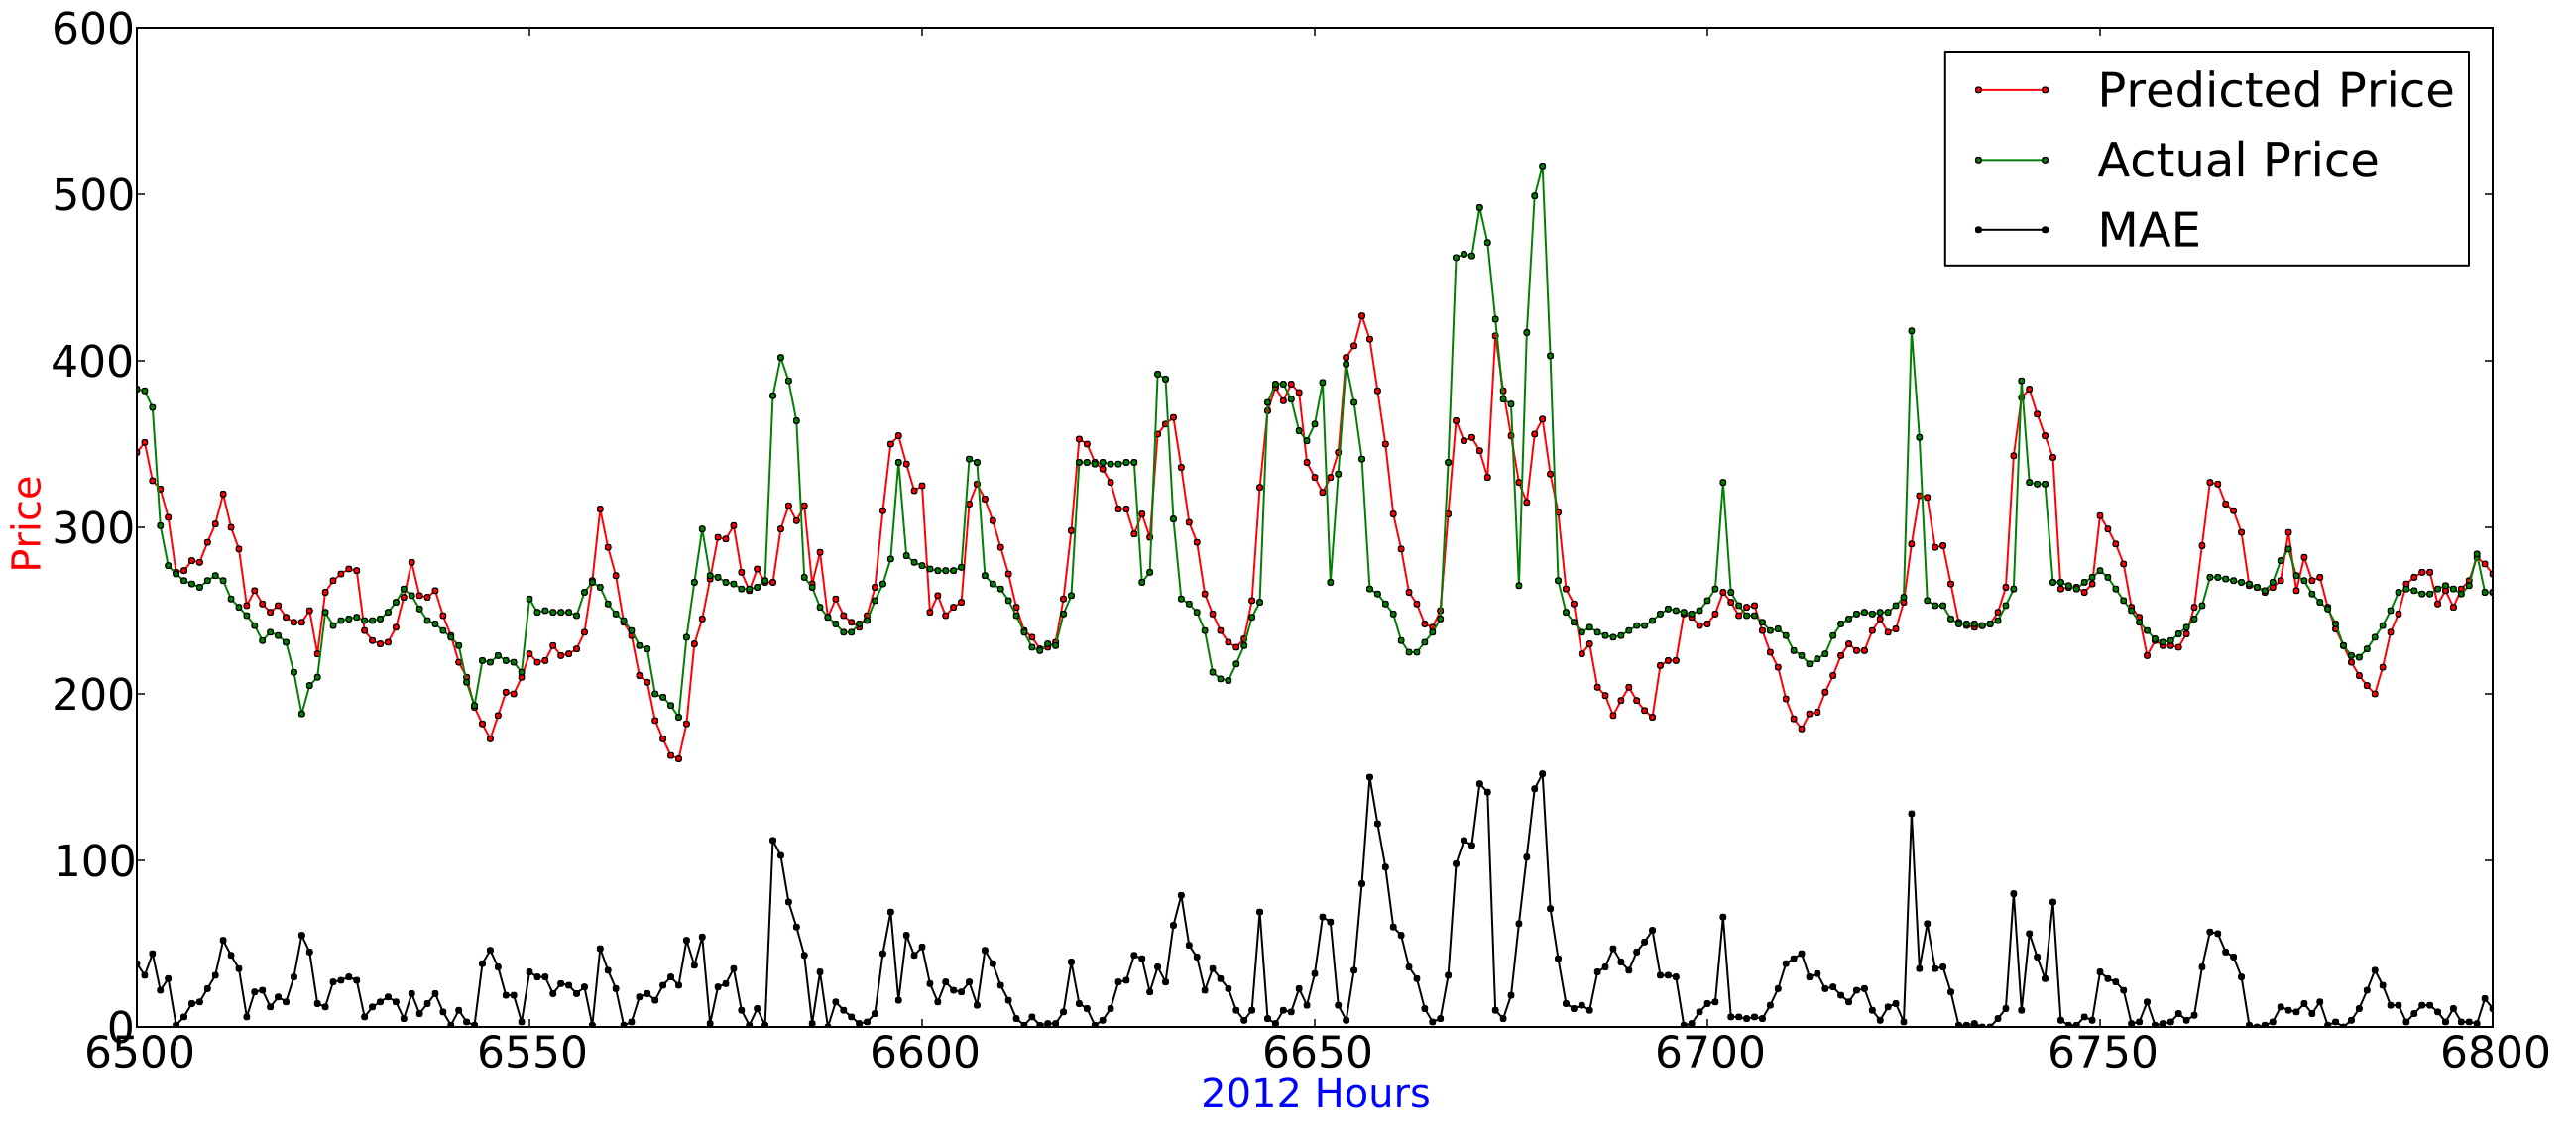
\includegraphics[width=\linewidth]{billeder/PriceExperimentalAnalysis/X3_Nr1_Best_skew_historical.png}
\caption{\#1 forecast from experiment three. Shows how well it follows the curve. The black curve in the bottom is the error for each prediction.}
\label{fig:X3_Best_With_MAE}
\end{figure}

In figure~\ref{fig:X2_X3_3800_4000} we see how the ANN has trouble predicting the unusual low values. This is the same for the experiment two prediction as it is for the experiment three prediction. The case we see in figure~\ref{fig:X2_X3_3800_4000} is what we hoped the calculated inputs would help the ANN to be better at predicting; since it has gained some knowledge about the immediate past. Experiment three also introduces more uneven curves where it fluctuates up and down compared to the prediction from experiment two which has smoother curves. This is because of the calculated inputs that add values that are interpreted into either a rising or a falling curve. Compared to the prediction from experiment two it does not have this knowledge and only relies on the interaction between the quantifiable parameters from experiment one.

\begin{figure}[H]
\centering
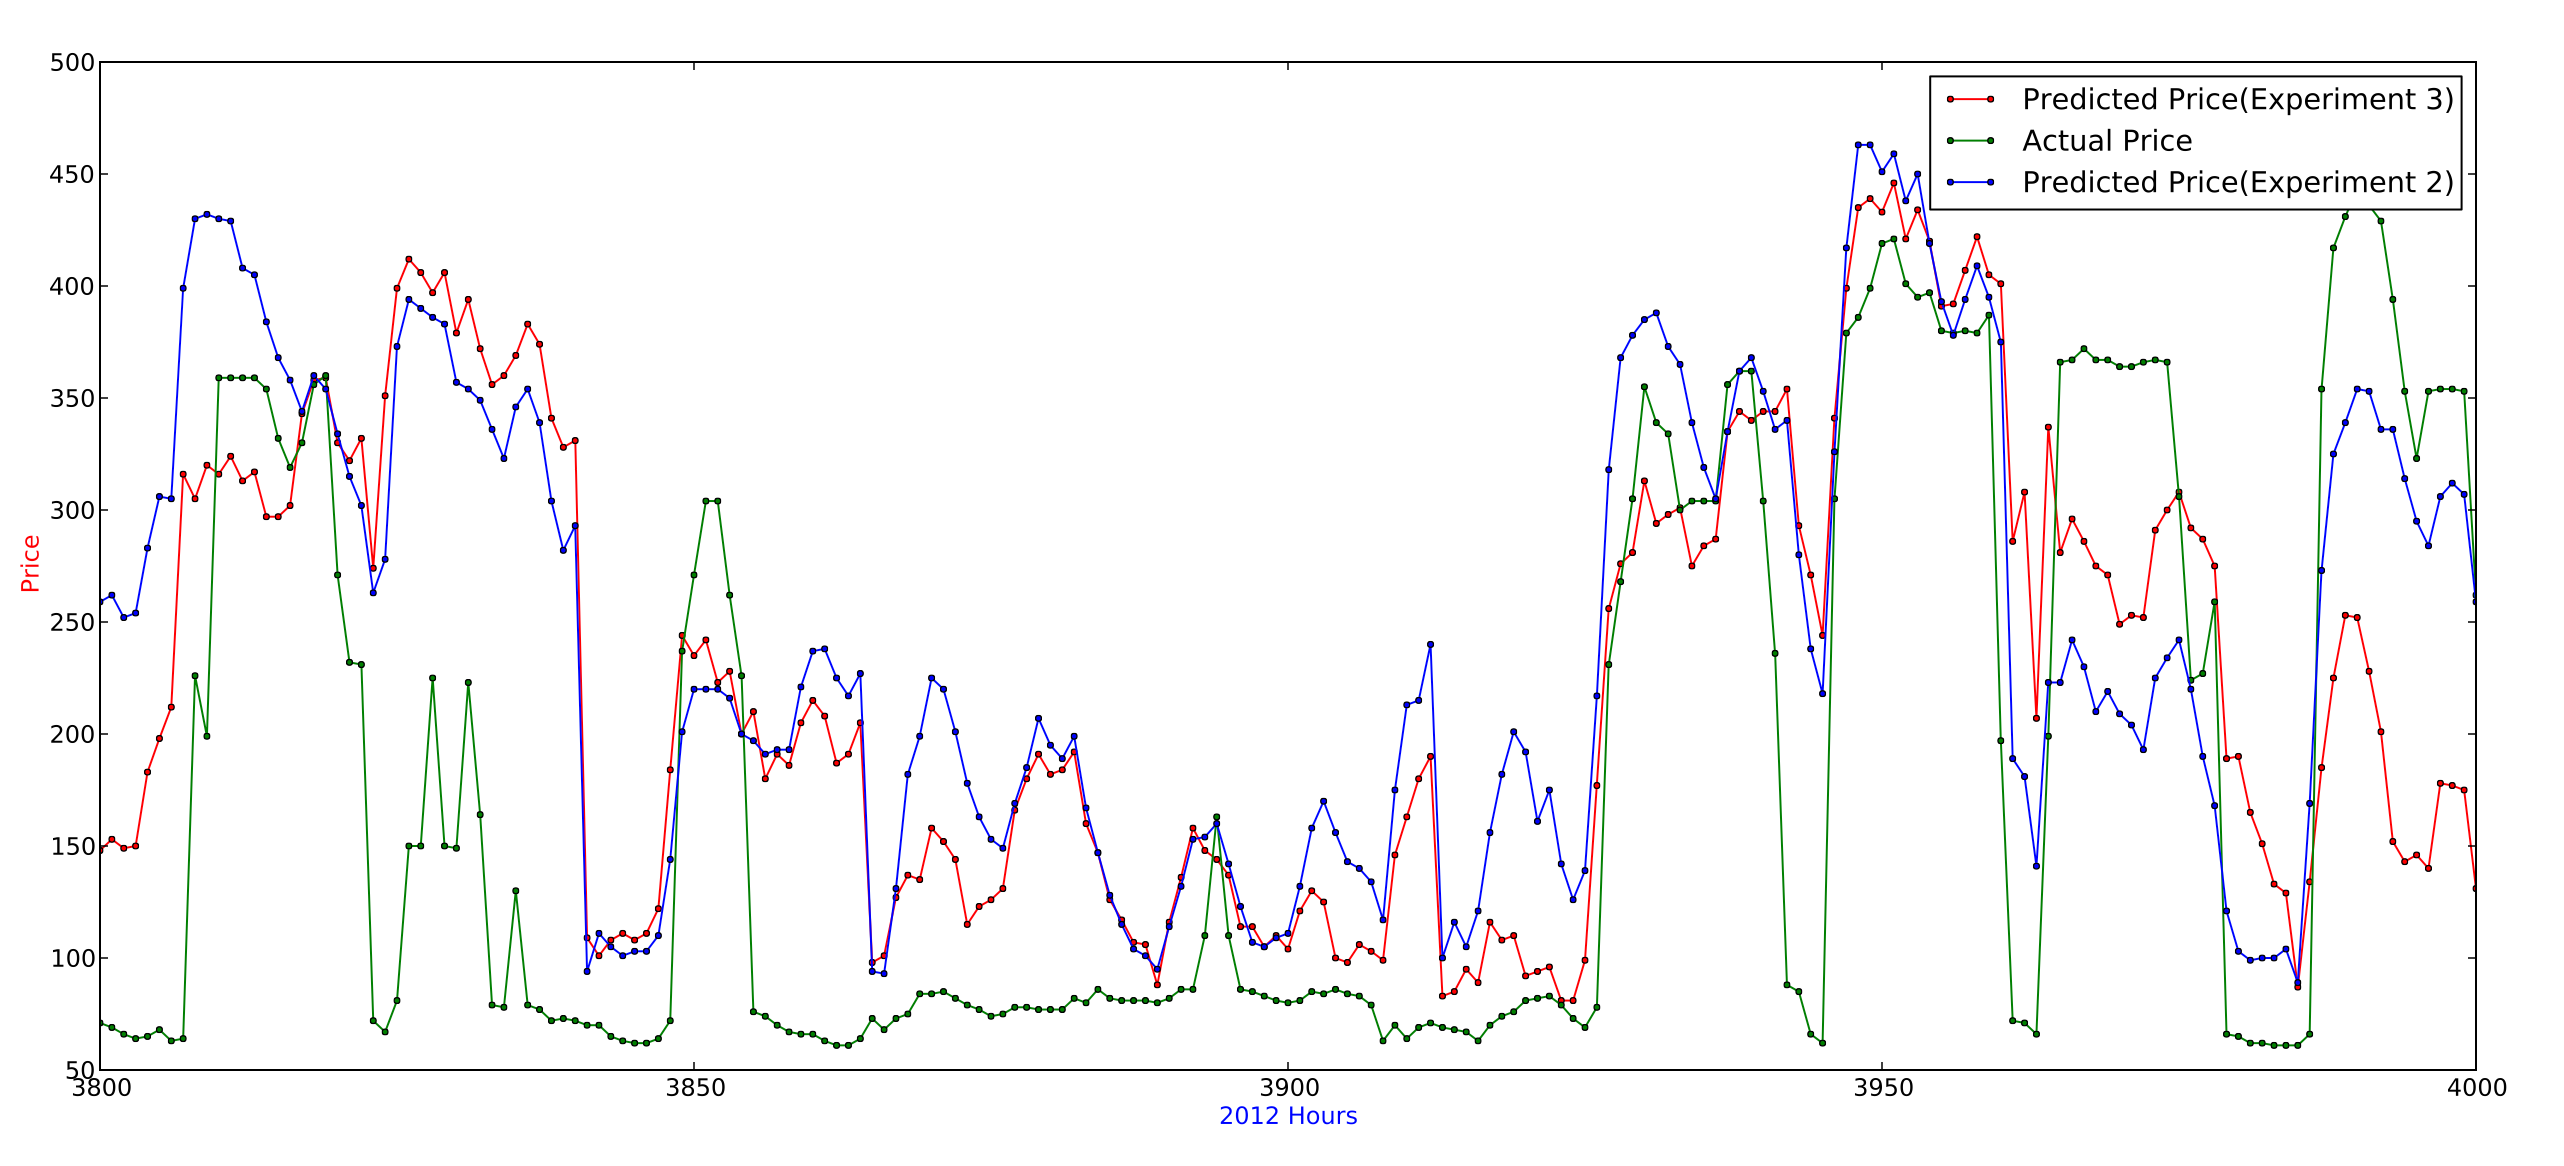
\includegraphics[width=\linewidth]{billeder/PriceExperimentalAnalysis/X2_X3_3800_4000.png}
\caption{A comparison of \#1 forecast from experiment two and three. This segment is from the middle of the year. (Skew, EWMA)}
\label{fig:X2_X3_3800_4000}
\end{figure}

If we apply all of the calculated inputs to the prediction we get Figure~\ref{fig:X2_X3_AllParameters_3800_4000}. In this figure we can see that it actually is able to drop to the lowest values in the dataset. On the other hand it has trouble rising from the low values which reintroduces the error but in the top of the dataset.

\begin{figure}[H]
\centering
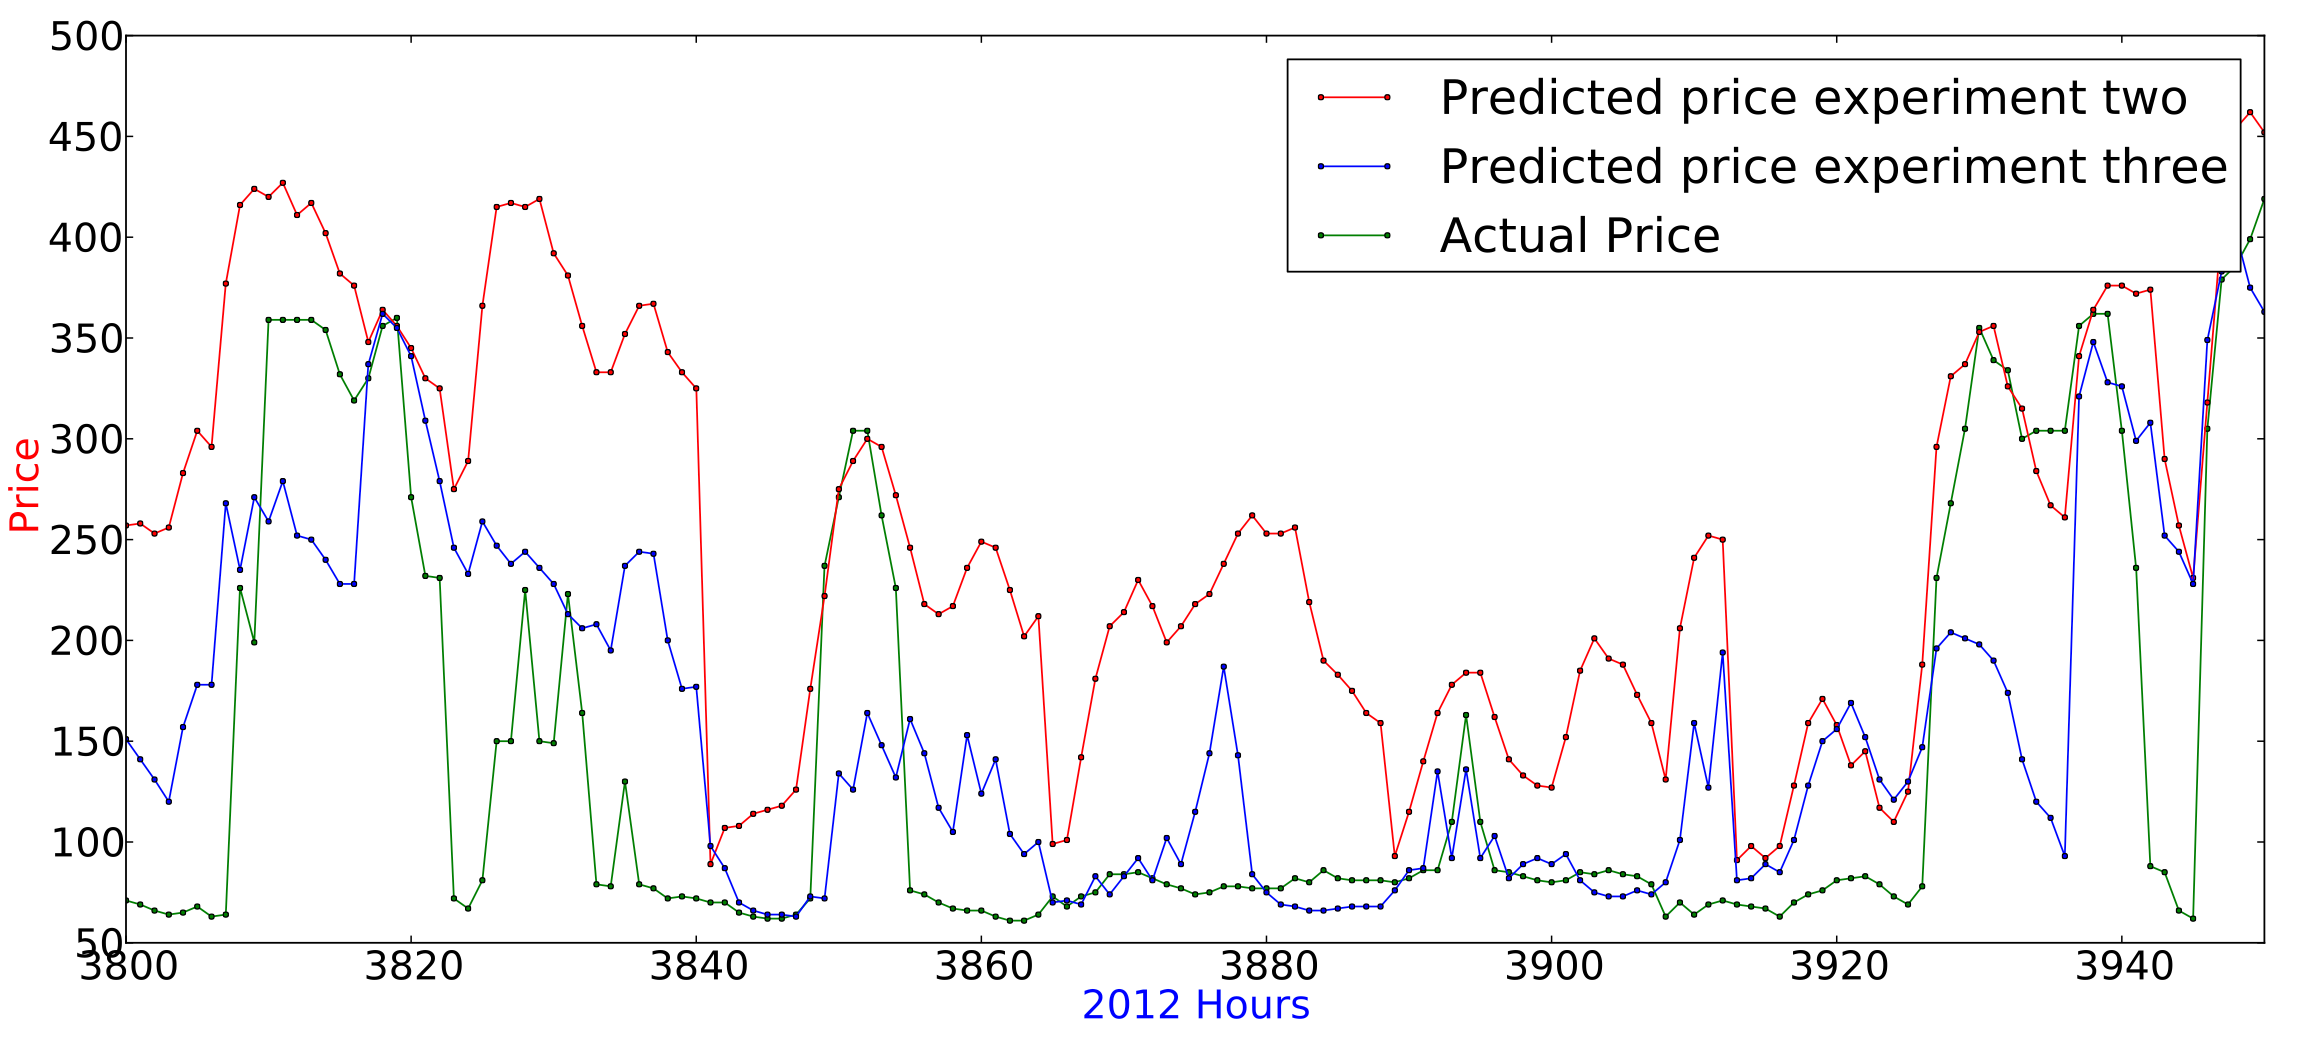
\includegraphics[width=\linewidth]{billeder/PriceExperimentalAnalysis/X2_X3_AllFeatures_3800_4000.png}
\caption{A comparison of \#1 forecast from experiment two and three. This segment is from the middle of the year. All features applied(Skew, Curve, EWMA, Scatter).}
\label{fig:X2_X3_AllParameters_3800_4000}
\end{figure}

\begin{figure}[H]
\centering
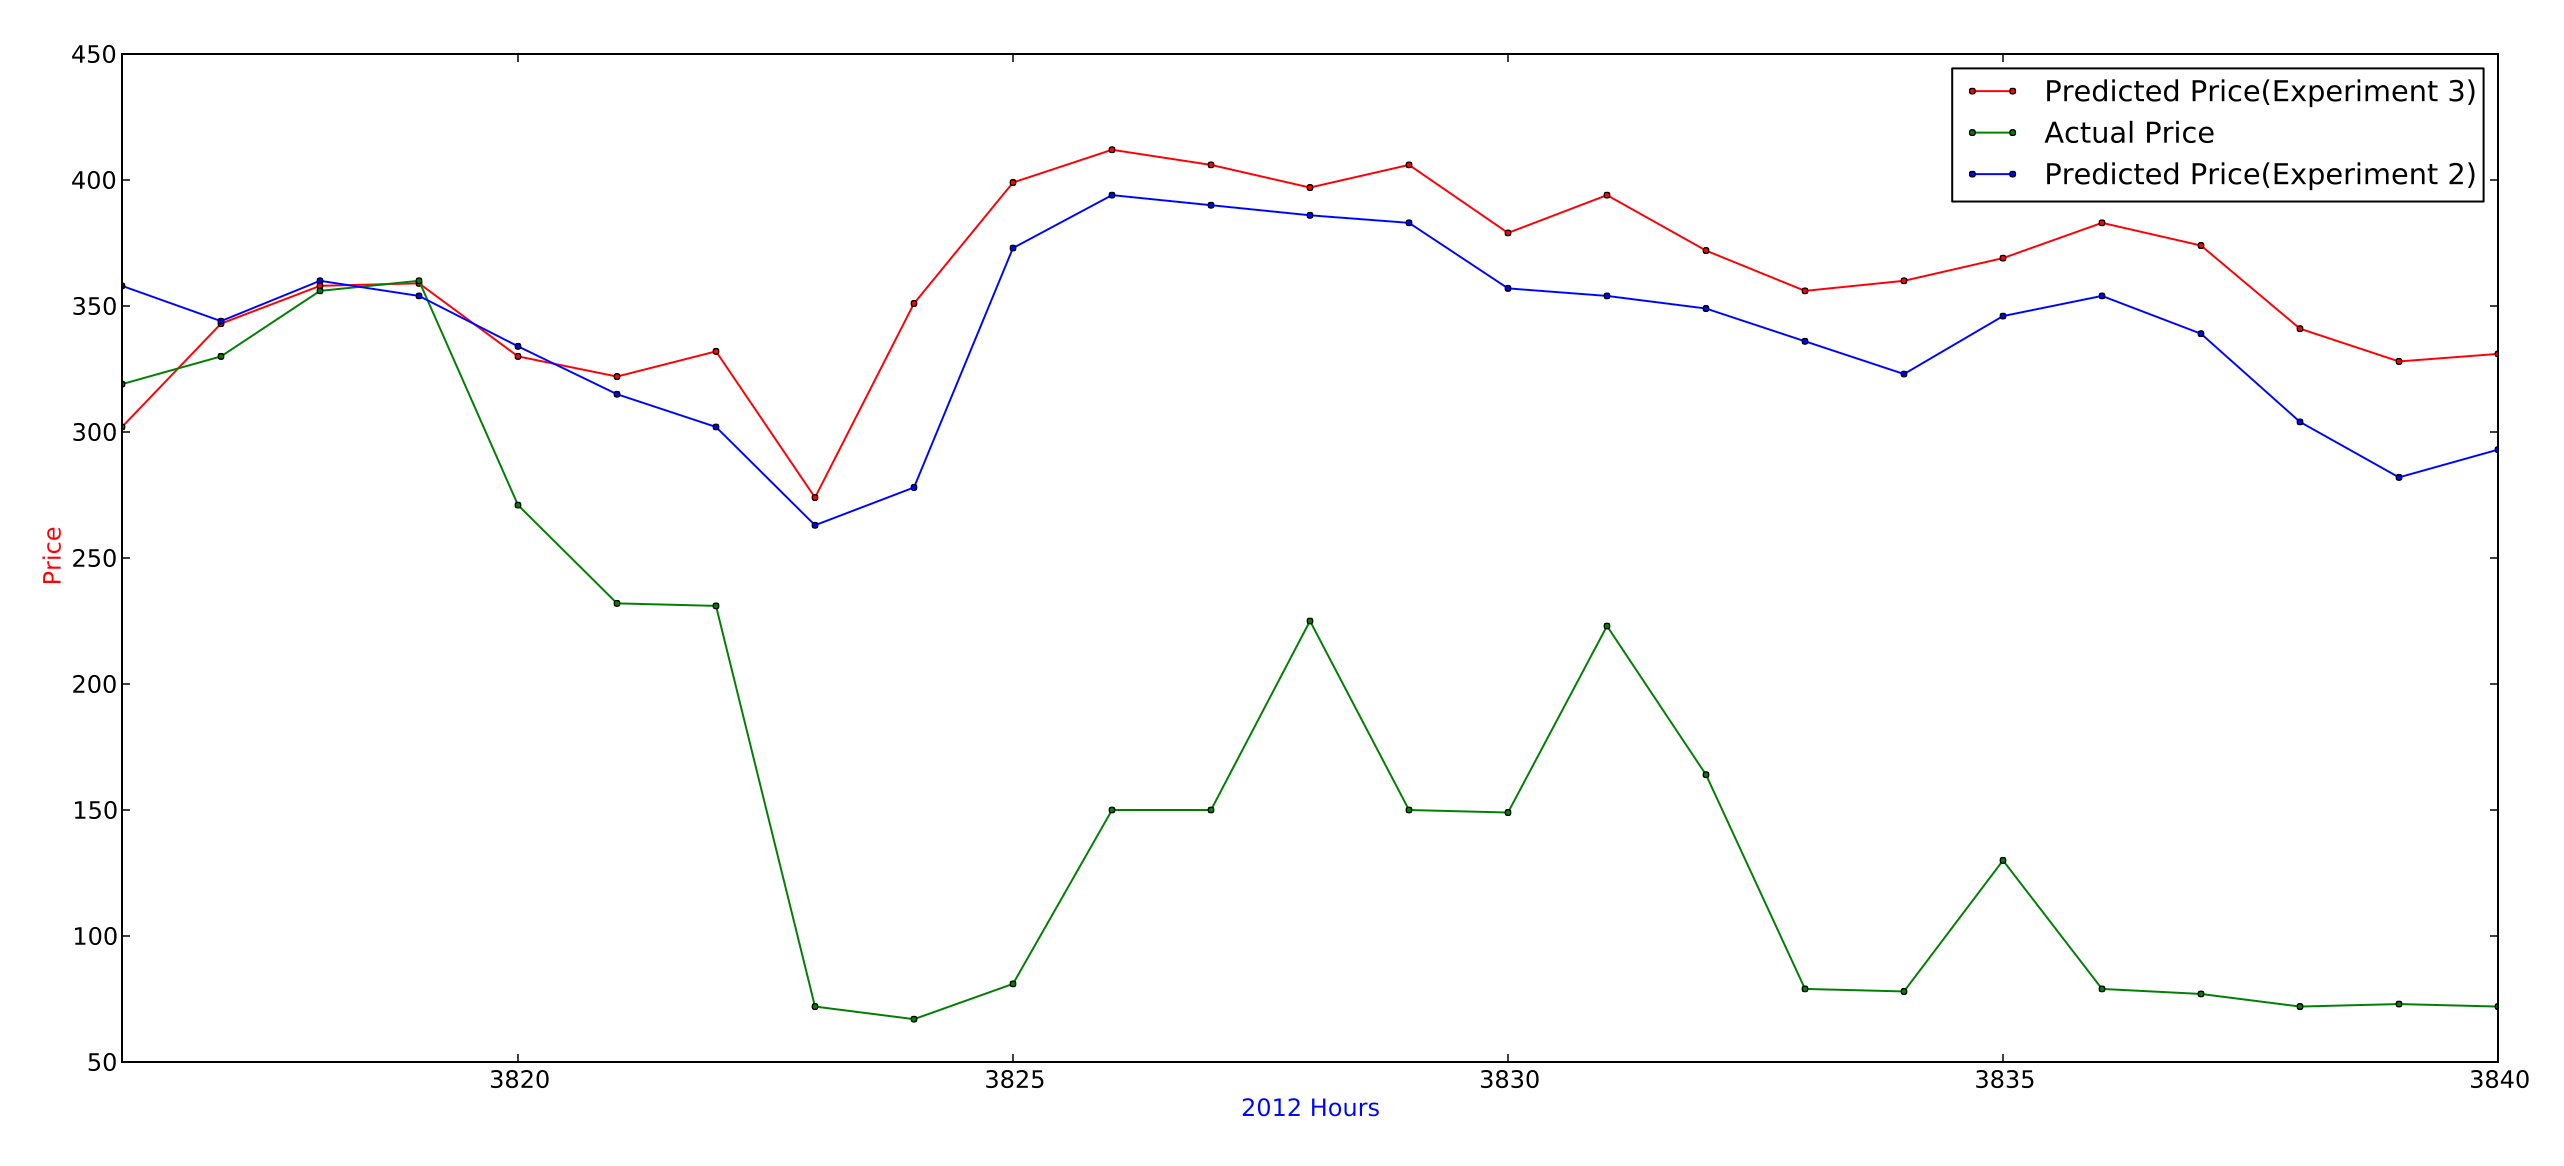
\includegraphics[width=\linewidth]{billeder/PriceExperimentalAnalysis/X2_X3_3816_3840.png}
\caption{\#1 from experiment two and three. 1 day-ahead prediction.}
\label{fig:X2_X3_3816_3840}
\end{figure}

Another problem with the calculated inputs are that making predictions with an ANN is about generalizing the inputs to reflect a mathematical function. If the ANN does not see enough examples of the calculated inputs throughout the training dataset it will not be able to make this generalization and thus not be able to use it efficiently in the predictions of the next 24 hours. If the first prediction in the next 24 hours is wrong (compared to the ideal prices) the calculated inputs can help elevate/decrease the error since the last known price is added to the calculation of these features (This can be seen in Figure~\ref{fig:X2_X3_3816_3840}). Also the calculated inputs are more or less unique throughout the whole year since the price does not follow a specific pattern that makes it harder to generalize the calculated inputs in the price prediction. The same was seen in experiment three for wind power in Section~\ref{sec:experimentThreeCalcInputs}.

The results in Table~\ref{table:Statistical2} and ~\ref{table:Statistical3} are control groups to show that other combinations of inputs has the same benefit from the calculated inputs.

\begin{figure}[H]
\centering
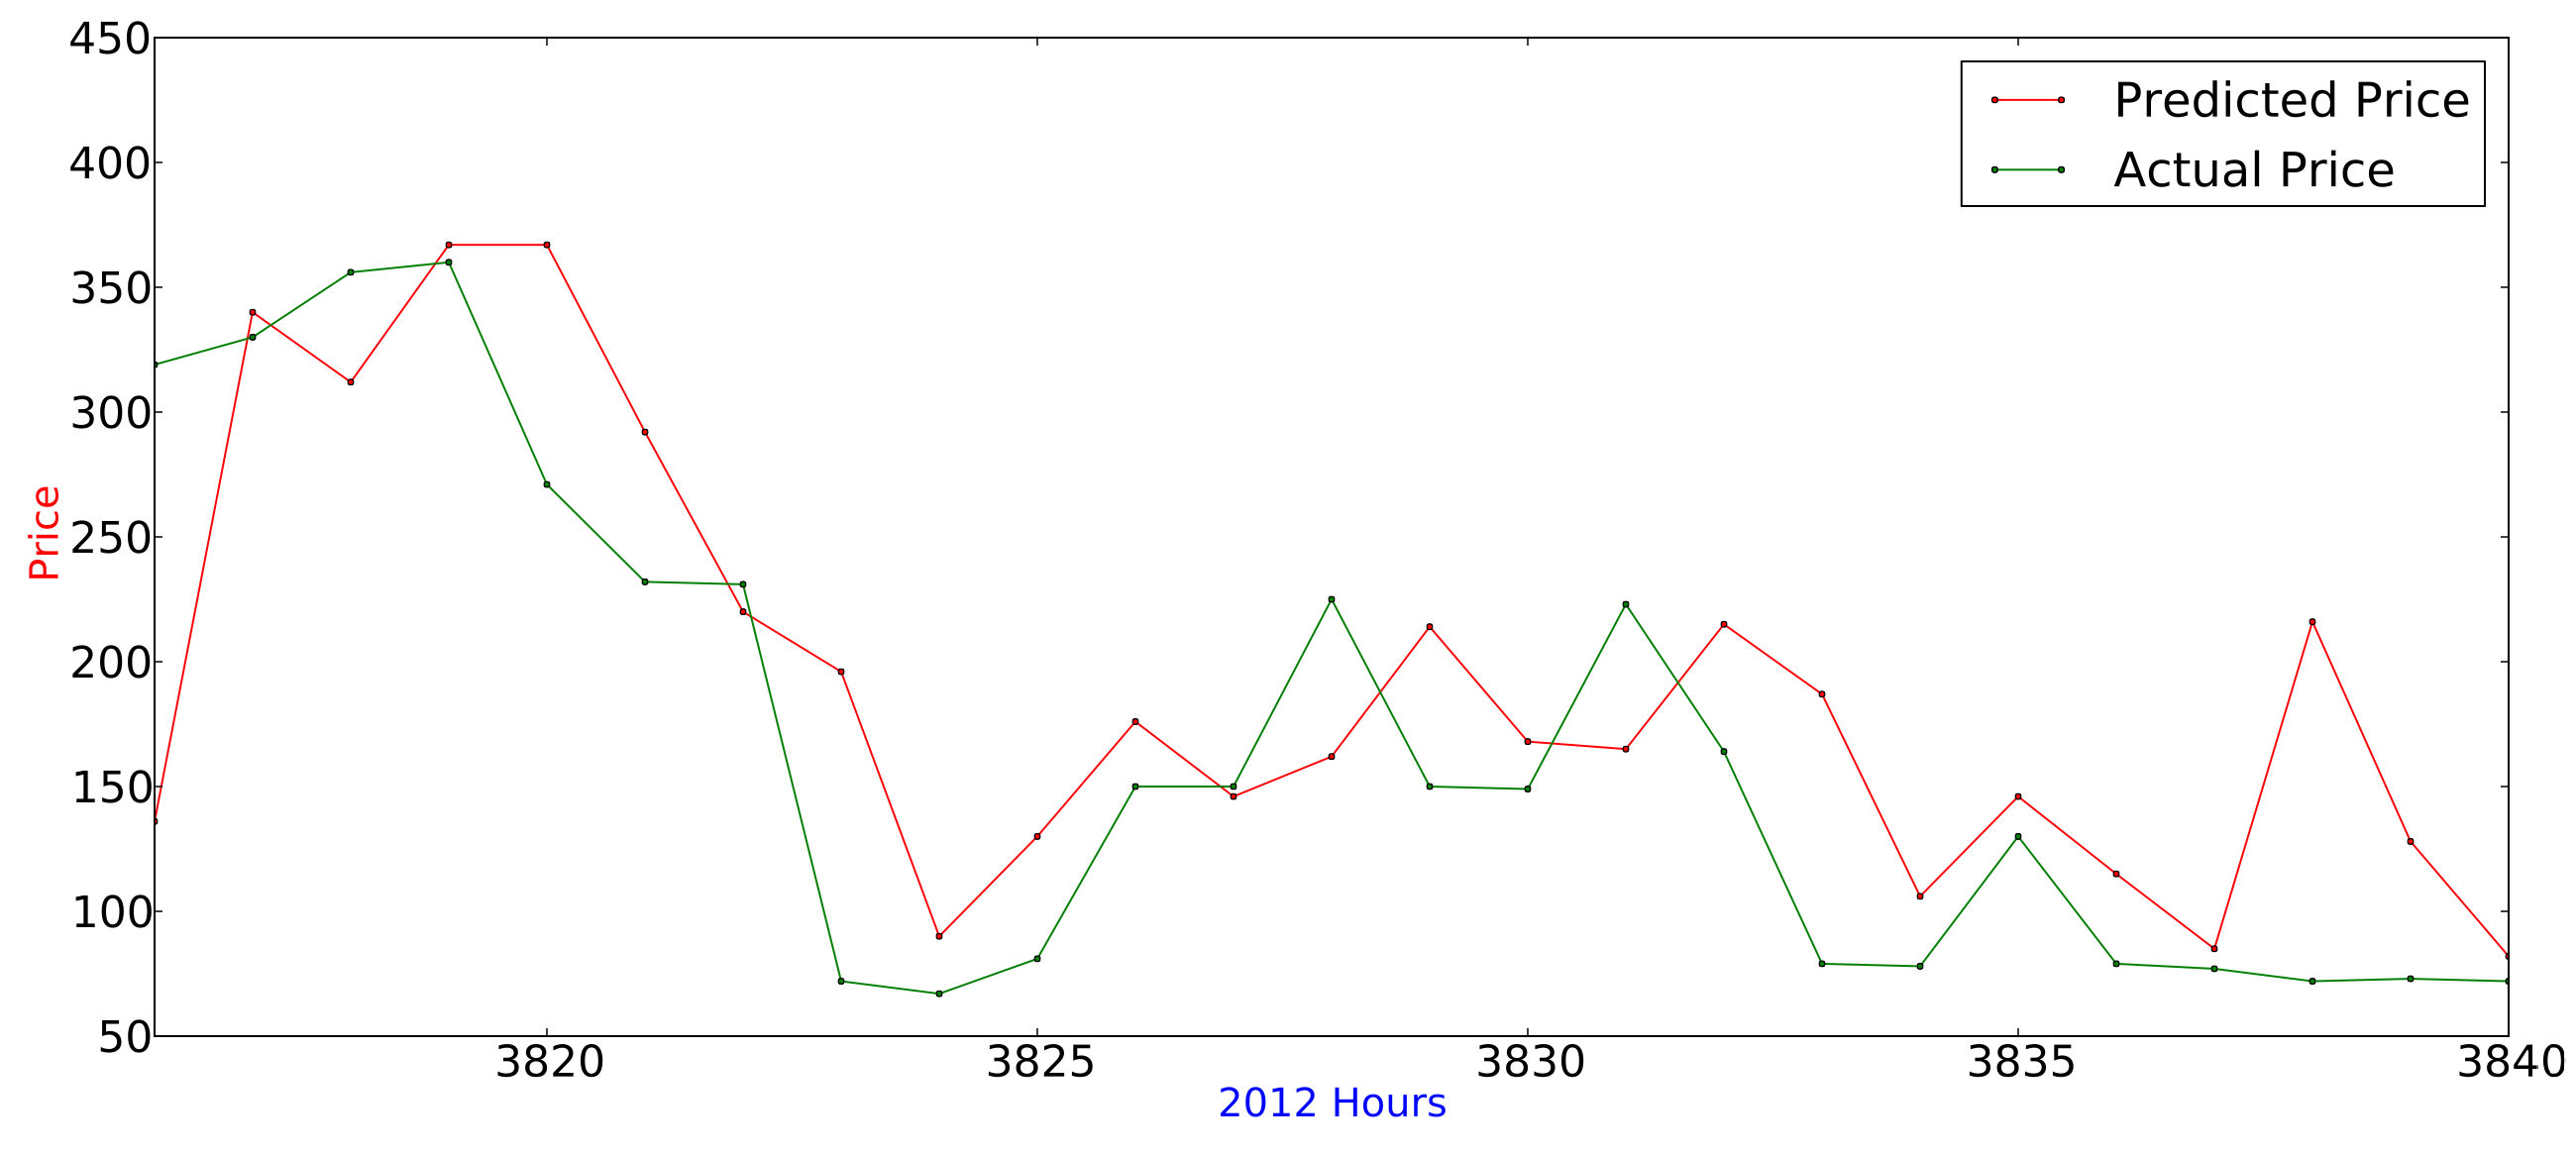
\includegraphics[width=\linewidth]{billeder/PriceExperimentalAnalysis/X2_X3_3816_3840_1hourAhead.png}
\caption{\#1 from experiment three. 1 hour-ahead prediction.}
\label{fig:X2_X3_3816_3840_1hourahead}
\end{figure}

\noindent Variables: Price, Demand, Wind Speed, Temperature, Time of Day (Matrix), Day of Week and Season of Year (Matrix)
\begin{table}[H]
\centering  % used for centering table
\resizebox{0.8\textwidth}{!}{
	\begin{tabular}{|c|c|c|c|c|c|c|c|c|} 
	\hline
	\# & Curve & Skew & Volatility & Scatter & \% CD & MAPE & MAE & \% Rank\\ [0.5ex] % inserts table 
	\hline                  % inserts single horizontal line
	1  &        & \x    & \x    &       & 67,0\% &  17,24\% & 45,11 & - \\ \hline
	2  &        &       & \x    &       & 66,5\% &  17,29\% & 45,24 & 0,28\% \\ \hline
	3  &  \x    & \x    & \x    &       & 66,0\% &  17,36\% & 45,43 & 0,7\% \\ \hline
	4  &  \x    &       &       &       & 69,2\% &  17,40\% & 45,53 & 0,92\% \\ \hline
	5  &  \x    & \x    &       & \x    & 68,5\% &  17,75\% & 46,45 & 2,98\% \\ \hline
	6  &  \x    & \x    &       &       & 69,3\% &  17,79\% & 46,56 & 3,2\% \\ \hline
	7  &        &       & \x    & \x    & 65,6\% &  17,87\% & 46,76 & 3,65\% \\ \hline
	8  &  \x    &       & \x    &       & 66,4\% &  17,91\% & 46,87 & 3,9\% \\ \hline
	9  &        & \x    & \x    & \x    & 65,4\% &  18,05\% & 47,25 & 4,73\% \\ \hline
	10 &        & \x    &       &       & 69,5\% &  18,30\% & 47,88 & 6,14\% \\ \hline
	11 &        &       &       & \x    & 68,2\% &  18,30\% & 47,88 & 6,14\% \\ \hline
	12 &  \x    & \x    & \x    & \x    & 65,6\% &  18,35\% & 48,01 & 6,43\% \\ \hline
	13 &  \x    &       & \x    & \x    & 65,4\% &  18,39\% & 48,13 & 6,68\% \\ \hline
	14 &        & \x    &       & \x    & 67,8\% &  18,50\% & 48,40 & 7,3\% \\ \hline
	15 &  \x    &       &       & \x    & 67,9\% &  18,98\% & 49,68 & 10,12\% \\ \hline
	\end{tabular}
}
\caption{Calculated inputs effect on result \#2 from experiment 1.} % title of Table
\label{table:Statistical2} % is used to refer this table in the text
\end{table}

\noindent Variables: Price, Demand, Wind Speed, Temperature, Time of Day (Matrix) and Month of Year (Matrix)
\begin{table}[H]
\centering  % used for centering table
\resizebox{0.8\textwidth}{!}{
	\begin{tabular}{|c|c|c|c|c|c|c|c|c|} 
	\hline
	\# & Curve & Skew & Volatility & Scatter & \% CD & MAPE & MAE & \% Rank\\ [0.5ex] % inserts table 
	\hline                  % inserts single horizontal line
	1  &        &       & \x    & \x    & 66,7\% &  17,25\% & 45,14 & - \\ \hline
	2  &        &       &       & \x    & 67,7\% &  17,40\% & 45,55 & 0,9\% \\ \hline
	3  &        & \x    &       &       & 69,6\% &  17,41\% & 45,56 & 0,92\% \\ \hline
	4  &        & \x    &       & \x    & 69,0\% &  17,43\% & 45,60 & 1,02\% \\ \hline
	5  &  \x    &       & \x    &       & 66,2\% &  17,54\% & 45,91 & 1,7\% \\ \hline
	6  &  \x    & \x    & \x    & \x    & 65,3\% &  17,56\% & 45,95 & 1,79\% \\ \hline
	7  &  \x    & \x    &       &       & 69,8\% &  17,57\% & 45,99 & 1,89\% \\ \hline
	8  &  \x    &       &       & \x    & 68,9\% &  17,63\% & 46,14 & 2,22\% \\ \hline
	9  &  \x    &       &       &       & 69,4\% &  17,80\% & 46,58 & 3,18\% \\ \hline
	10 &  \x    & \x    &       & \x    & 68,3\% &  17,91\% & 46,87 & 3,82\% \\ \hline
	11 &        &       & \x    &       & 67,4\% &  17,95\% & 46,98 & 4,08\% \\ \hline
	12 &        & \x    & \x    & \x    & 66,0\% &  17,97\% & 47,02 & 4,16\% \\ \hline
	13 &  \x    & \x    & \x    &       & 66,3\% &  17,99\% & 47,08 & 4,3\% \\ \hline
	14 &  \x    &       & \x    & \x    & 66,6\% &  18,32\% & 47,94 & 6,2\% \\ \hline
	15 &        & \x    & \x    &       & 66,9\% &  18,33\% & 47,98 & 6,29\% \\ \hline
	\end{tabular}
}
\caption{Calculated inputs effect on result \#3 from experiment 1.} % title of Table
\label{table:Statistical3} % is used to refer this table in the text
\end{table}

\subsubsection{Calculated inputs effect on a simple dataset}
To test the benefit of the calculated inputs on a dataset that only contains the price and demand we conducted two more experiments - one with trimming(1\%) and one without trimming. The different approaches to calculated inputs are again historical volatility, skewness, slope calculation and the scatter approach from \cite{singhal2011electricity}. 

Test \#1 shown in Table~\ref{table:price_consumption_x3} shows the calculated inputs applied on a dataset without trimming. The original test from experiment one can be seen in the price results in Appendix~\ref{sec:priceResultAppendix} \#106 and it gave us an MAE of 89 for the dataset only consisting of price and demand. If we compare it to this test we see and improvement of 21.24\%. The most notable trend in the results in Table~\ref{table:price_consumption_x3} is that nearly all of the scatter prices are the top results. 

\begin{table}[H]
\centering  % used for centering table
\resizebox{0.8\textwidth}{!}{
	\begin{tabular}{|c|c|c|c|c|c|c|c|c|} 
	\hline
	\# & Curve & Skew & Volatility & Scatter & \% CD & MAPE & MAE & \% Rank\\ [0.5ex] % inserts table 
	\hline                  % inserts single horizontal line
	1  &        &       &       & \x    & 60,3\% &  27,92\% & 73,43 & - \\ \hline
	2  &  \x    &       &       & \x    & 60,5\% &  29,07\% & 76,45 & 4,11\% \\ \hline
	3  &        &       & \x    &       & 53,4\% &  29,47\% & 77,50 & 5,54\% \\ \hline
	4  &  \x    &       & \x    & \x    & 59,1\% &  29,48\% & 77,54 & 5,6\% \\ \hline
	5  &        & \x    &       & \x    & 60,7\% &  30,10\% & 79,17 & 7,82\% \\ \hline
	6  &        &       & \x    & \x    & 59,7\% &  30,67\% & 80,67 & 9,86\% \\ \hline
	7  &        & \x    & \x    & \x    & 58,7\% &  30,74\% & 80,85 & 10,11\% \\ \hline
	8  &  \x    & \x    & \x    & \x    & 58,6\% &  31,17\% & 81,97 & 11,63\% \\ \hline
	9  &        & \x    &       &       & 54,0\% &  32,08\% & 84,37 & 14,9\% \\ \hline
	10 &  \x    & \x    &       & \x    & 58,6\% &  32,27\% & 84,86 & 15,57\% \\ \hline
	11 &  \x    & \x    & \x    &       & 52,4\% &  32,89\% & 86,49 & 17,79\% \\ \hline
	12 &  \x    &       & \x    &       & 53,7\% &  33,06\% & 86,95 & 18,41\% \\ \hline
	13 &        & \x    & \x    &       & 52,9\% &  33,65\% & 88,50 & 20,52\% \\ \hline
	14 &  \x    &       &       &       & 53,6\% &  33,94\% & 89,26 & 21,57\% \\ \hline
	15 &  \x    & \x    &       &       & 53,0\% &  36,60\% & 96,24 & 31,07\% \\ \hline
	\end{tabular}
}
\caption{Calculated inputs on Price \& demand with no trim.} % title of Table
\label{table:price_consumption_x3} % is used to refer this table in the text
\end{table}

The best results for the same experiment but with 1\% trim can be seen in Table~\ref{table:price_consumption_x3_1pTrim}. The results are improved but the trimming did not help as significantly as we saw in experiment two. The scatter price approach again takes the best positions which indicates that the network itself can calculate the connection to previous prices when no meteorological factors are included. It can also be seen that from 1-7 the 1\% trim outperforms the prediction without trimming but thereafter trimming becomes the worst of the two.

\begin{table}[H]
\centering  % used for centering table
\resizebox{0.8\textwidth}{!}{
	\begin{tabular}{|c|c|c|c|c|c|c|c|c|} 
	\hline
	\# & Curve & Skew & Volatility & Scatter & \% CD & MAPE & MAE & \% Rank\\ [0.5ex] % inserts table 
	\hline                  % inserts single horizontal line
	1  &        &       &       & \x    & 55,5\% &  26,09\% & 68,28 & - \\ \hline
	2  &  \x    & \x    &       & \x    & 56,0\% &  26,52\% & 69,40 & 1,63\% \\ \hline
	3  &        & \x    &       & \x    & 55,6\% &  26,81\% & 70,17 & 2,77\% \\ \hline
	4  &  \x    &       &       & \x    & 56,2\% &  26,85\% & 70,28 & 2,93\% \\ \hline
	5  &        & \x    &       &       & 52,4\% &  27,57\% & 72,16 & 5,68\% \\ \hline
	6  &  \x    & \x    &       &       & 52,1\% &  28,78\% & 75,31 & 10,29\% \\ \hline
	7  &  \x    &       &       &       & 51,1\% &  29,48\% & 77,14 & 12,97\% \\ \hline
	8  &  \x    &       & \x    & \x    & 52,7\% &  35,86\% & 93,86 & 37,46\% \\ \hline
	9  &  \x    & \x    & \x    & \x    & 53,2\% &  36,00\% & 94,21 & 37,98\% \\ \hline
	10 &        &       & \x    & \x    & 52,8\% &  36,31\% & 95,02 & 39,17\% \\ \hline
	11 &        & \x    & \x    & \x    & 51,7\% &  37,37\% & 97,79 & 43,22\% \\ \hline
	12 &        &       & \x    &       & 50,9\% &  42,76\% & 111,91 & 63,9\% \\ \hline
	13 &        & \x    & \x    &       & 49,9\% &  44,29\% & 115,91 & 69,76\% \\ \hline
	14 &  \x    &       & \x    &       & 50,4\% &  44,64\% & 116,83 & 71,11\% \\ \hline
	15 &  \x    & \x    & \x    &       & 49,9\% &  45,40\% & 118,82 & 74,03\% \\ \hline
	\end{tabular}
}
\caption{Calculated inputs on Price \& demand with 1\% trim.} % title of Table
\label{table:price_consumption_x3_1pTrim} % is used to refer this table in the text
\end{table}

The most noteworthy is that the two results (with and without trimming) are very similar; the one with trimming is actually worse when the historical volatility strategy is applied but the top results show better results with trimming which was expected due to the findings in experiment two of electricity prices. We can conclude that trimming has less effect on the dataset than we saw in our experiment from earlier and it is even worse on the results from \#7-\#15. In Figure~\ref{fig:X3_Price_Consump_NoTrim} and ~\ref{fig:X3_Price_Consump_1pTrim} show the comparison between the best prediction for with and without trimming. The trimming having less effect is expressed in the comparison in the similarities between the two. 

\begin{figure}[H]
\centering
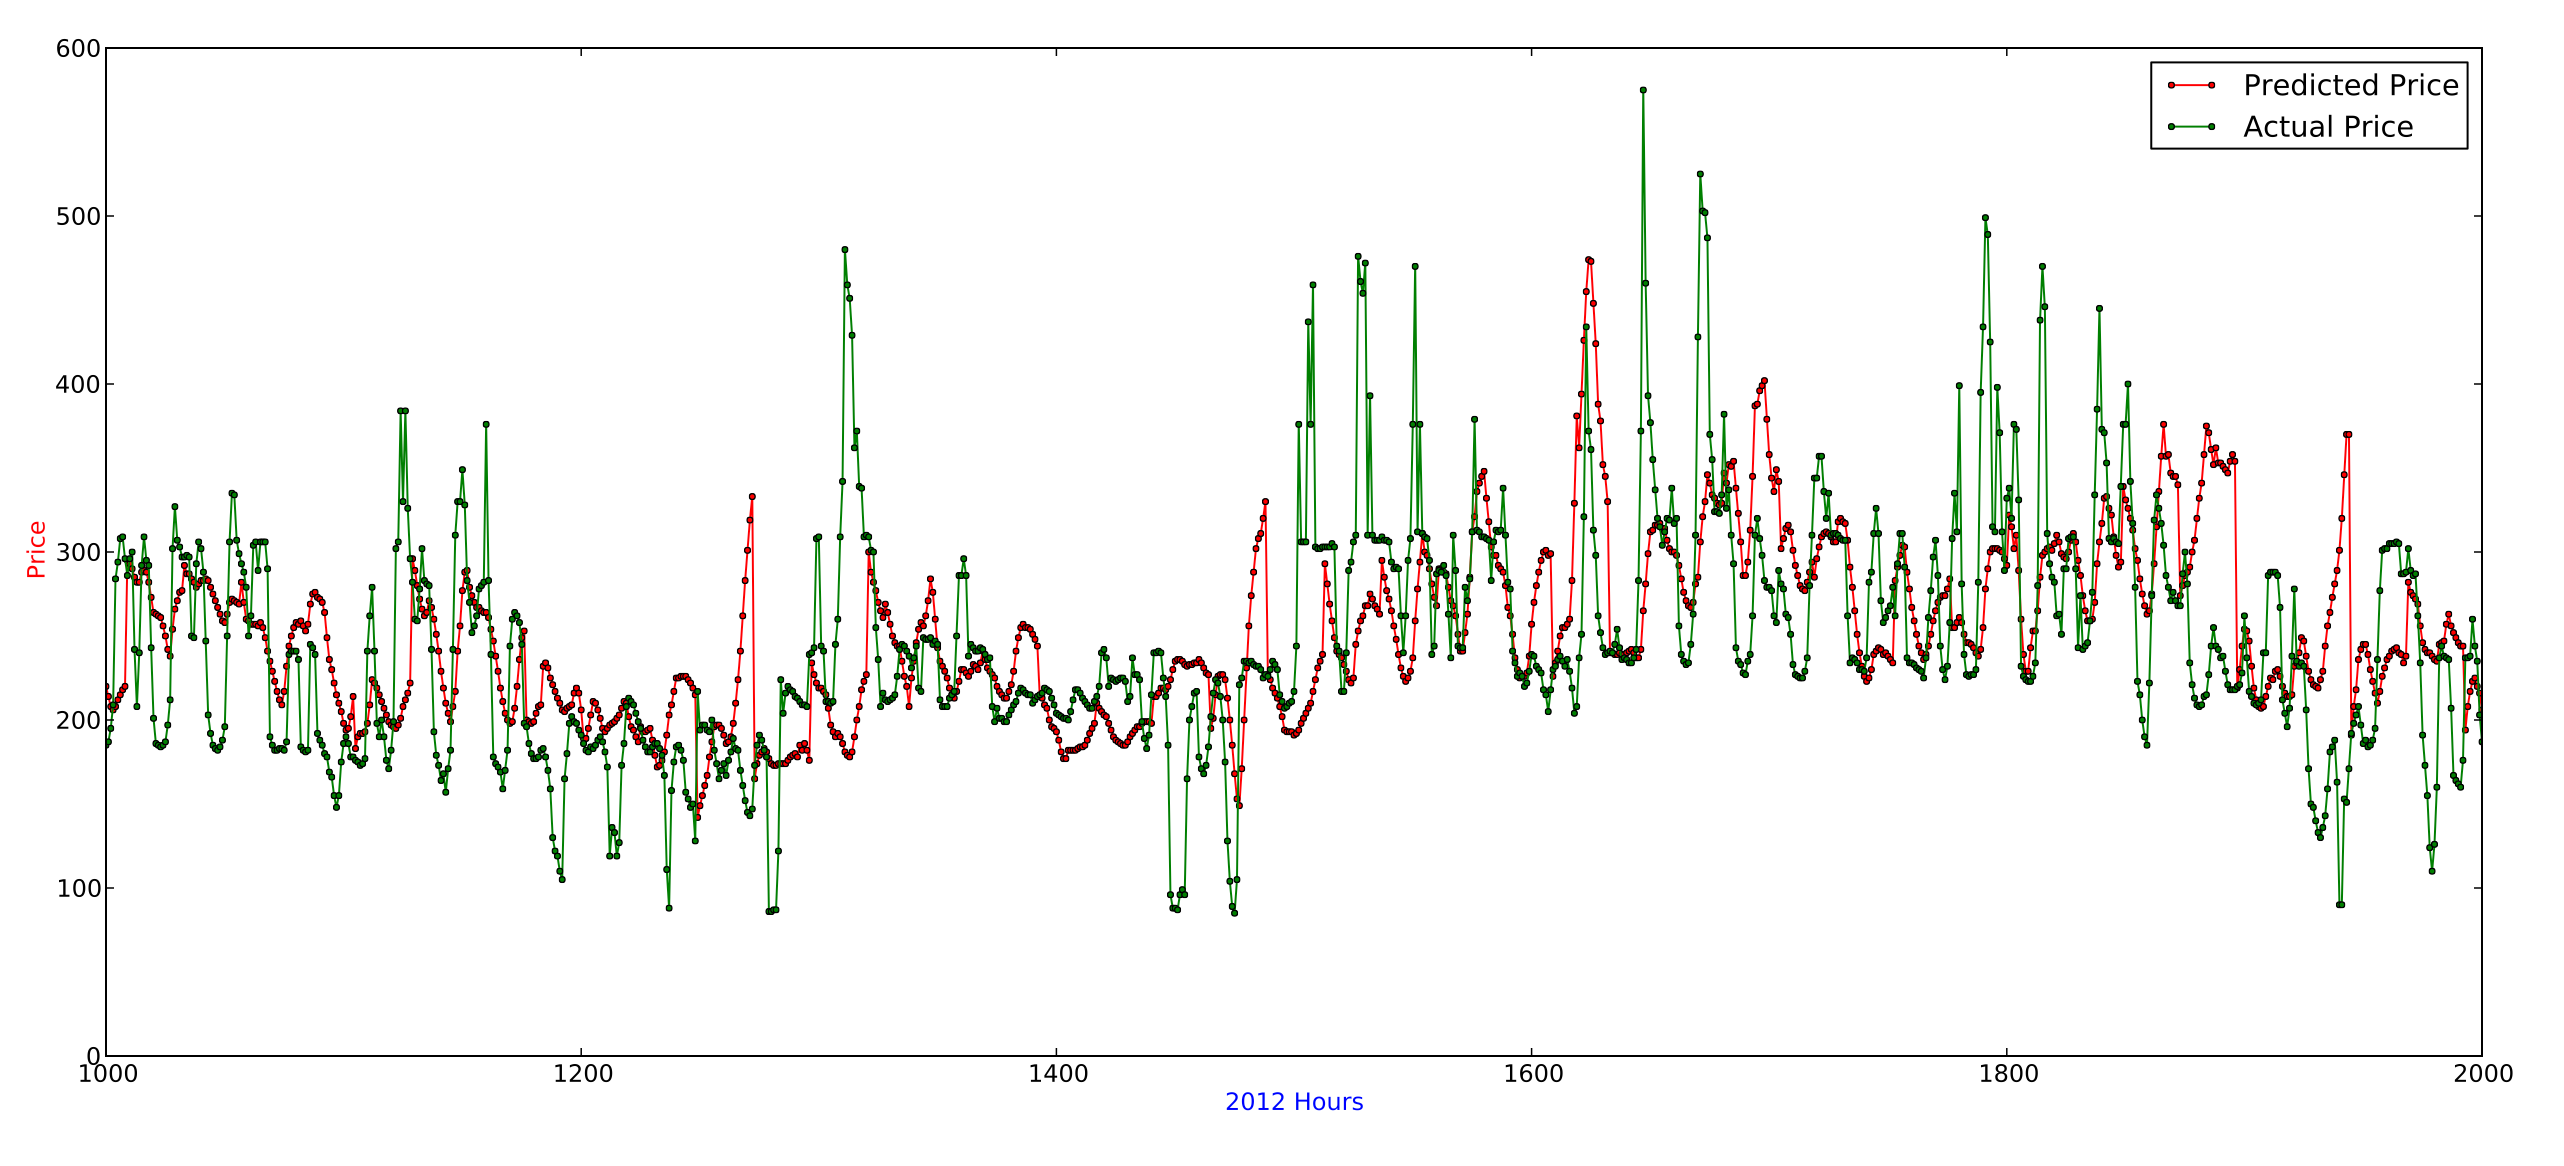
\includegraphics[width=\linewidth]{billeder/PriceExperimentalAnalysis/X3_Price_Consump_1pTrim.png}
\caption{Price and demand with scatter and 1\% trim.)}
\label{fig:X3_Price_Consump_1pTrim}
\end{figure}

\begin{figure}[H]
\centering
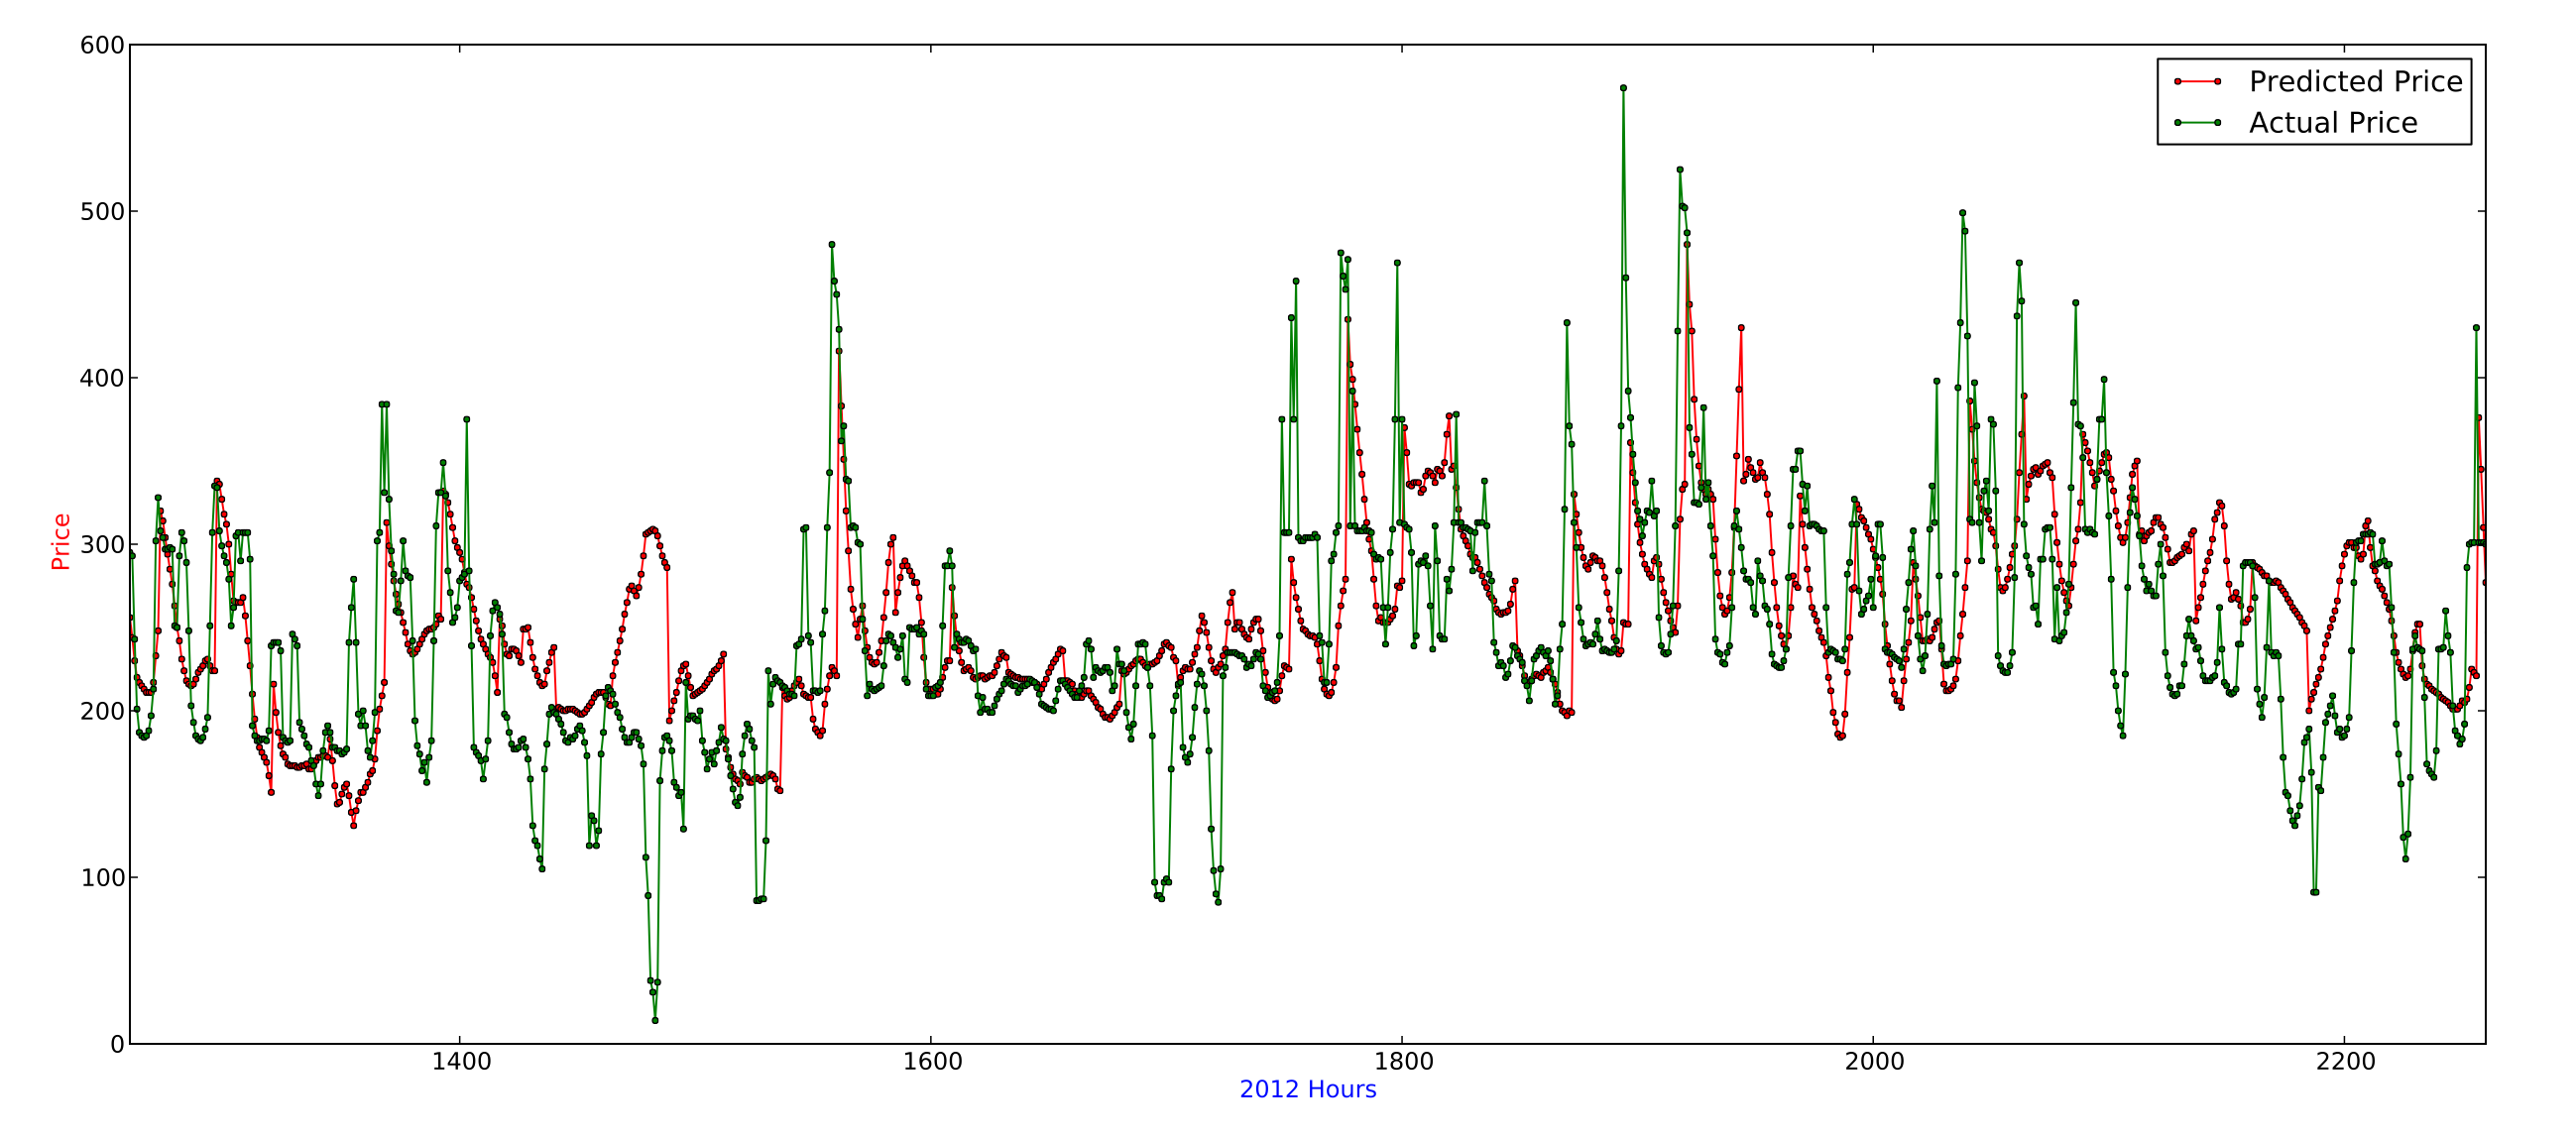
\includegraphics[width=\linewidth]{billeder/PriceExperimentalAnalysis/X3_Price_Consump_NoTrim.png}
\caption{Price and demand with scatter and no trim.}
\label{fig:X3_Price_Consump_NoTrim}
\end{figure}

\subsubsection{Clone scatter experiment from literature}
The network has the ability of calculating the influence of previous hours itself. This is described in~\cite{singhal2011electricity} and for comparison of our own calculated input approach we have attempted to use their approach (which we have denoted as scatter). The setup includes price, demand, time of day, day of week and scatter. We have done the prediction both with 1\% and no trim as they did in the text (can be transferred to small spikes and large spikes). The results can be seen in Table~\ref{table:scatter_text_no_trim} and ~\ref{table:scatter_text_1p_trim}. The results with trimming and the best strategies gives us a result of 52,04 MAE which is 14,75\% worse than the best result from Table~\ref{table:Statistical1}. The results without trimming is 71,51 MAE which is 25.19\% worse than the best result from Table~\ref{table:Top20Prices} in experiment one. We cannot compare the results directly to the paper since they only present a prediction of 48 hours and they do not describe whether this is on unseen data or it is on the same dataset as they trained on. Neither do we know whether they simulate the full 48 hour prediction or they perform it 1-hour at a time.

Comparing results is difficult due to lack of information on experimental environments and influential factors for that specific market. We will in the discussion of our results elaborate on our experience with this. 

\noindent Variables: Price, Demand, Change in demand, Time of Day, Day of Week and with no trimming
\begin{table}[H]
\centering  % used for centering table
\resizebox{0.8\textwidth}{!}{
	\begin{tabular}{|c|c|c|c|c|c|c|c|c|} 
	\hline
	\# & Curve & Skew & Volatility & Scatter & \% CD & MAPE & MAE & \% Rank\\ [0.5ex] % inserts table 
	\hline                  % inserts single horizontal line
	1  &        & \x    &       & \x    & 60,2\% &  27,19\% & 71,51 & - \\ \hline
	2  &        &       & \x    & \x    & 61,3\% &  27,82\% & 73,17 & 2,33\% \\ \hline
	3  &        & \x    & \x    & \x    & 61,1\% &  30,16\% & 79,31 & 10,92\% \\ \hline
	4  &        &       &       & \x    & 60,2\% &  30,50\% & 80,20 & 12,16\% \\ \hline
	5  &  \x    & \x    & \x    & \x    & 59,7\% &  31,19\% & 82,03 & 14,73\% \\ \hline
	6  &  \x    &       & \x    & \x    & 58,6\% &  34,15\% & 89,82 & 25,61\% \\ \hline
	7  &  \x    &       &       & \x    & 60,0\% &  35,84\% & 94,26 & 31,83\% \\ \hline
	8  &  \x    & \x    &       & \x    & 58,8\% &  36,09\% & 94,90 & 32,72\% \\ \hline
	\end{tabular}
}
\caption{Scatter text~\cite{singhal2011electricity} with other calculated inputs and no trim} % title of Table
\label{table:scatter_text_no_trim} % is used to refer this table in the text
\end{table}


\noindent Variables: Price, Demand, Change in demand, Time of Day, Day of Week and with 1\% trimming
\begin{table}[H]
\centering  % used for centering table
\resizebox{0.8\textwidth}{!}{
	\begin{tabular}{|c|c|c|c|c|c|c|c|c|} 
	\hline
	\# & Curve & Skew & Volatility & Scatter & \% CD & MAPE & MAE & \% Rank\\ [0.5ex] % inserts table 
	\hline                  % inserts single horizontal line
	1  &  \x    & \x    &       & \x    & 63,6\% &  19,88\% & 52,04 & - \\ \hline
	2  &  \x    &       & \x    & \x    & 65,8\% &  19,91\% & 52,12 & 0,15\% \\ \hline
	3  &        & \x    & \x    & \x    & 66,4\% &  20,34\% & 53,22 & 2,27\% \\ \hline
	4  &        & \x    &       & \x    & 63,7\% &  20,64\% & 54,02 & 3,8\% \\ \hline
	5  &  \x    &       &       & \x    & 66,8\% &  20,85\% & 54,55 & 4,83\% \\ \hline
	6  &        &       & \x    & \x    & 63,0\% &  21,32\% & 55,80 & 7,23\% \\ \hline
	7  &        &       &       & \x    & 64,0\% &  21,52\% & 56,33 & 8,24\% \\ \hline
	8  &  \x    & \x    & \x    & \x    & 59,2\% &  23,66\% & 61,92 & 18,99\% \\ \hline
	\end{tabular}
}
\caption{Scatter text~\cite{singhal2011electricity} with other calculated inputs and 1\% trim} % title of Table
\label{table:scatter_text_1p_trim} % is used to refer this table in the text
\end{table}

\subsubsection{Conclusion}
The calculated inputs slightly helped the curve analysis by adding extra characteristics. The best improvement gave a result that was 4.54\% better than the same combination in experiment two. The results indicate an improvement by using the calculated inputs for further analysis of the dataset and at worst the prediction does not suffer any decrease in accuracy from using it.

The results from the simple dataset (last known price and demand) showed us that if we apply calculated inputs to this dataset it will improve significantly which emphasizes that the calculated inputs do bring extra information to the ANN so that it can approach the target better. The improvement makes it as good as the best combination from experiment one. The downside to this is that we are not able to improve it further. So it gets stuck with that error margin. We conducted the same trial with a 1\% trimmed dataset and here we saw no improvement. It shows that our calculated inputs can improve simple datasets better than complex ones.

The last part was a comparison with the paper~\cite{singhal2011electricity} where they have a setup which we copied in this experiment. Their setup did a good job of predicting the price but our setup gave a better result. We cannot compare the results directly due to a lack of information on how they conducted their trials. We have done on a dataset with and without trimming applied. In this case the trimmed dataset gave a better result.

\newpage
\subsection{Experiment Four - Black Box Optimization}
\label{sec:priceExperimentFour}
We here show the impacts of epochs used to train the network and the size of the training dataset. We also show how the time dimension of doing these tests are affected by these parameters. Black box optimization also covers the number of hidden layers and the neuron count in these. We assume that the number of layers and neurons are optimized best possible through a pruning algorithm as described in Section~\ref{sec:testProcedure} and in Section~\ref{sec:pruning}. Therefore we will not be covering it here but the numbers have been added in the previous experiments and will be here as well. 

\subsubsection{Variables}
All of these tests were conducted using the best combination seen in table ~\ref{table:Statistical1}. Giving us the following combination:
\begin{itemize}
	\item Price
	\item Demand
	\item Wind Speed
	\item Temperature
	\item Time of Day (Matrix)
	\item Day of Week (Matrix)
	\item Season of Year (Matrix)
	\item Skewness
	\item EWMA
\end{itemize}

The following parameters were tested:

\begin{itemize}
	\item Epochs from 1 to 3000
	\item Dataset sizes equivalent to 1/4, 1/2, 3/4 and a 1/1 year
\end{itemize}

\subsubsection{Hypothesis}
We expect the results from these tests to show that the time used to make a years prediction will increase with the number of epochs and it will increase with the size of the dataset. We expect too few number and too many number of epochs to significantly worsen the result. The best results from the dataset test is expected to be 1/4 year or 1/2 year sizes. These assumptions are based on what we described in the Forecasting Model chapter~\ref{ch:forecastingModel}.

\subsubsection{Results}
The results from Table~\ref{table:Dataset_size} shows the impact of increasing the size of the training dataset. The influence of increasing the size shows a deviation of 7,19\%. It shows that the best result are the size equivalent to half a year. The second best are the one year prediction which might be because we included the seasonal parameters as we showed in experiment one; where the addition of the Month of Year(MoY) parameter increased the performance of a one year training set. The one we have used throughout the preceding results are the third best and gave a result that was 6,46\% worse than the best thus we might be able to increase some of the scores from earlier experiments if we use a dataset consisting of data from half a year. Another interesting fact here is how the time to a prediction increases linearly with the amount of entries in the dataset - from 232 seconds (3.9 minutes) to 844 seconds (14.1 minutes).

\begin{table}[H]
\centering  % used for centering table
\resizebox{0.8\textwidth}{!}{
	\begin{tabular}{|c|c|c|c|c|c|c|c|c|} % centered columns (7 columns)
	\hline
	\# & Entries & Time(seconds) & H1 & H2 & \% CD & MAPE & MAE & \% Rank\\ [0.5ex] % inserts table 
	\hline                  % inserts single horizontal line
	1  & 4378 & 397,28 & 6  & 11 & 70,1\% & 17,71\% & 46,34 & - \\ \hline
	2  & 8756 & 844,68 & 12 & 5  & 70,7\% & 18,27\% & 47,82 & 3,19\% \\ \hline
	3  & 2189 & 232,87 & 6  & 18 & 68,6\% & 18,85\% & 49,33 & 6,46\% \\ \hline
	4  & 6567 & 677,33 & 14 & 6  & 67,3\% & 18,98\% & 49,67 & 7,19\% \\ \hline
	\end{tabular}
}
\caption{The results from the dataset size test.} % title of Table
\label{table:Dataset_size} % is used to refer this table in the text
\end{table}

\begin{figure}[H]
\centering
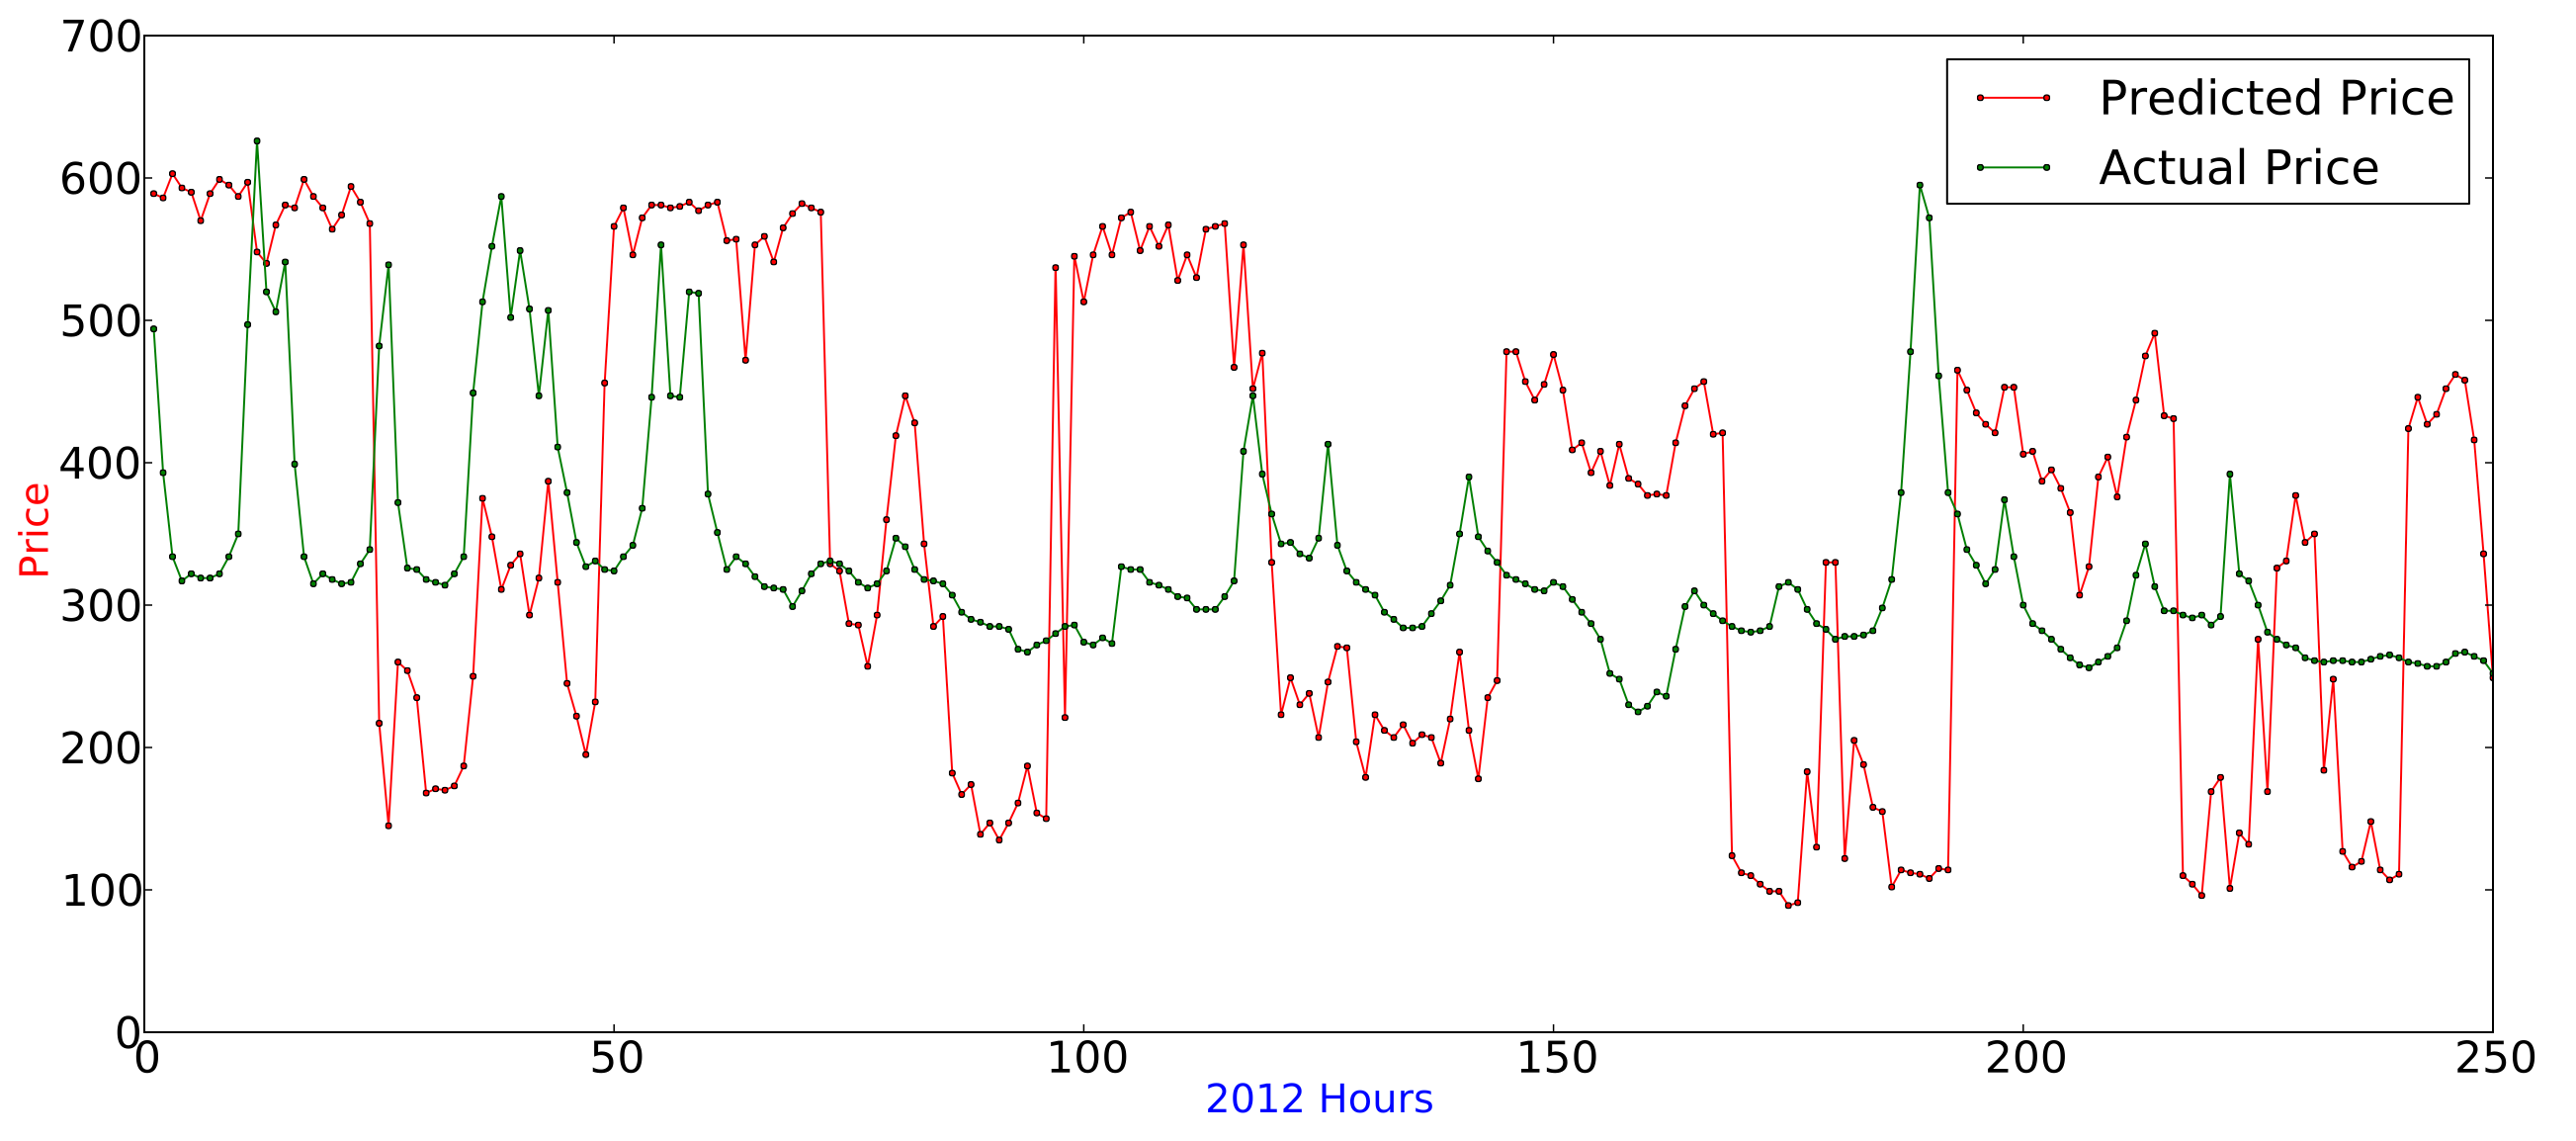
\includegraphics[width=\linewidth]{billeder/PriceExperimentalAnalysis/1EpochTraining.png}
\caption{Shows how the predictions are done when the network is trained for 1 epoch before every prediction}
\label{fig:1epoch}
\end{figure}

In Table~\ref{table:Epochs} we see the effects of epochs used when training the network. We see a tendency that values between 100 and 1000 are the best number of epochs to use in this network. 40 epochs also perform very well which are a bit surprising since the number of epochs used to train the network reflects how many iterations the network undergoes to find the best match between the weights. The under fitting of the weights can be seen in 1 epoch training(\#27 in ~\ref{table:Epochs}) where the network gets one attempt to correct the weights and find a generalization of the parameters (which would be a lucky guess if that happened). The 1 epoch run can be seen in figure~\ref{fig:1epoch}.


\begin{table}[H]
\centering  % used for centering table
\resizebox{0.8\textwidth}{!}{
	\begin{tabular}{|c|c|c|c|c|c|c|c|c|} % centered columns (7 columns)		
	\hline
	\# & Epochs & Time(seconds) & H1 & H2 & \% CD & MAPE & MAE & \% Rank \\ [0.5ex] % inserts table 
	\hline                  % inserts single horizontal line
	1  & 500  & 450,19 & 12 & 11 & 67,1\% & 17,26\% & 45,17 & - \\ \hline
	2  & 600  & 375,02 & 7  & 11 & 68,4\% & 17,63\% & 46,14 & 2,16\% \\ \hline
	3  & 900  & 415,28 & 8  & 3  & 68,3\% & 18,08\% & 47,32 & 4,77\% \\ \hline
	4  & 1100 & 566,83 & 10 & 5  & 67,4\% & 18,11\% & 47,40 & 4,95\% \\ \hline
	5  & 200  & 264,03 & 14 & 8  & 66,1\% & 18,31\% & 47,92 & 6,09\% \\ \hline
	6  & 100  & 213,95 & 14 & 11 & 65,8\% & 18,39\% & 48,13 & 6,55\% \\ \hline
	7  & 1600 & 807,21 & 6  & 17 & 68,9\% & 18,43\% & 48,23 & 6,78\% \\ \hline
	8  & 300  & 315,01 & 14 & 10 & 66,4\% & 18,50\% & 48,41 & 7,17\% \\ \hline
	9  & 1200 & 676,83 & 10 & 9  & 66,8\% & 18,63\% & 48,74 & 7,91\% \\ \hline
	10 & 40   & 185,18 & 17 & 8  & 64,8\% & 18,85\% & 49,34 & 9,24\% \\ \hline
	11 & 400  & 345,01 & 12 & 8  & 67,1\% & 18,87\% & 49,37 & 9,3\% \\ \hline
	12 & 1800 & 1496,67 & 5  & 1  & 70,1\% & 19,03\% & 49,80 & 10,26\% \\ \hline
	13 & 800  & 518,7  & 8  & 16 & 66,8\% & 19,16\% & 50,15 & 11,02\% \\ \hline
	14 & 1000 & 612,22 & 8  & 18 & 66,3\% & 19,36\% & 50,67 & 12,19\% \\ \hline
	15 & 1300 & 877,29 & 13 & 13 & 66,0\% & 19,40\% & 50,78 & 12,42\% \\ \hline
	16 & 1500 & 691,92 & 7  & 8  & 66,0\% & 19,42\% & 50,82 & 12,52\% \\ \hline
	17 & 2400 & 2510,23 & 6  & 11 & 66,4\% & 19,71\% & 51,58 & 14,2\% \\ \hline
	18 & 2200 & 3296,05 & 10 & 25 & 64,5\% & 19,76\% & 51,72 & 14,5\% \\ \hline
	19 & 3000 & 3600,85 & 7  & 19 & 64,2\% & 19,91\% & 52,09 & 15,33\% \\ \hline
	20 & 700  & 471,98 & 7  & 20 & 64,9\% & 19,97\% & 52,26 & 15,7\% \\ \hline
	21 & 2000 & 3035,47 & 13 & 16 & 64,8\% & 20,46\% & 53,56 & 18,57\% \\ \hline
	22 & 20   & 175,38 & 19 & 8  & 63,6\% & 20,52\% & 53,69 & 18,87\% \\ \hline
	23 & 1400 & 978,75 & 12 & 18 & 64,8\% & 20,79\% & 54,41 & 20,46\% \\ \hline
	24 & 2800 & 3202,93 & 7  & 15 & 63,4\% & 21,09\% & 55,20 & 22,2\% \\ \hline
	25 & 2600 & 3286,09 & 11 & 9  & 65,2\% & 22,04\% & 57,69 & 27,73\% \\ \hline
	26 & 10   & 177,02 & 14 & 6  & 60,4\% & 22,45\% & 58,75 & 30,07\% \\ \hline
	27 & 1    & 168,82 & 15 & 10 & 50,3\% & 46,81\% & 122,50 & 171,2\% \\ \hline
	\end{tabular}
}
\caption{The results from the epochs experiment.} % title of Table
\label{table:Epochs} % is used to refer this table in the text
\end{table}

\begin{figure}[H]
\centering
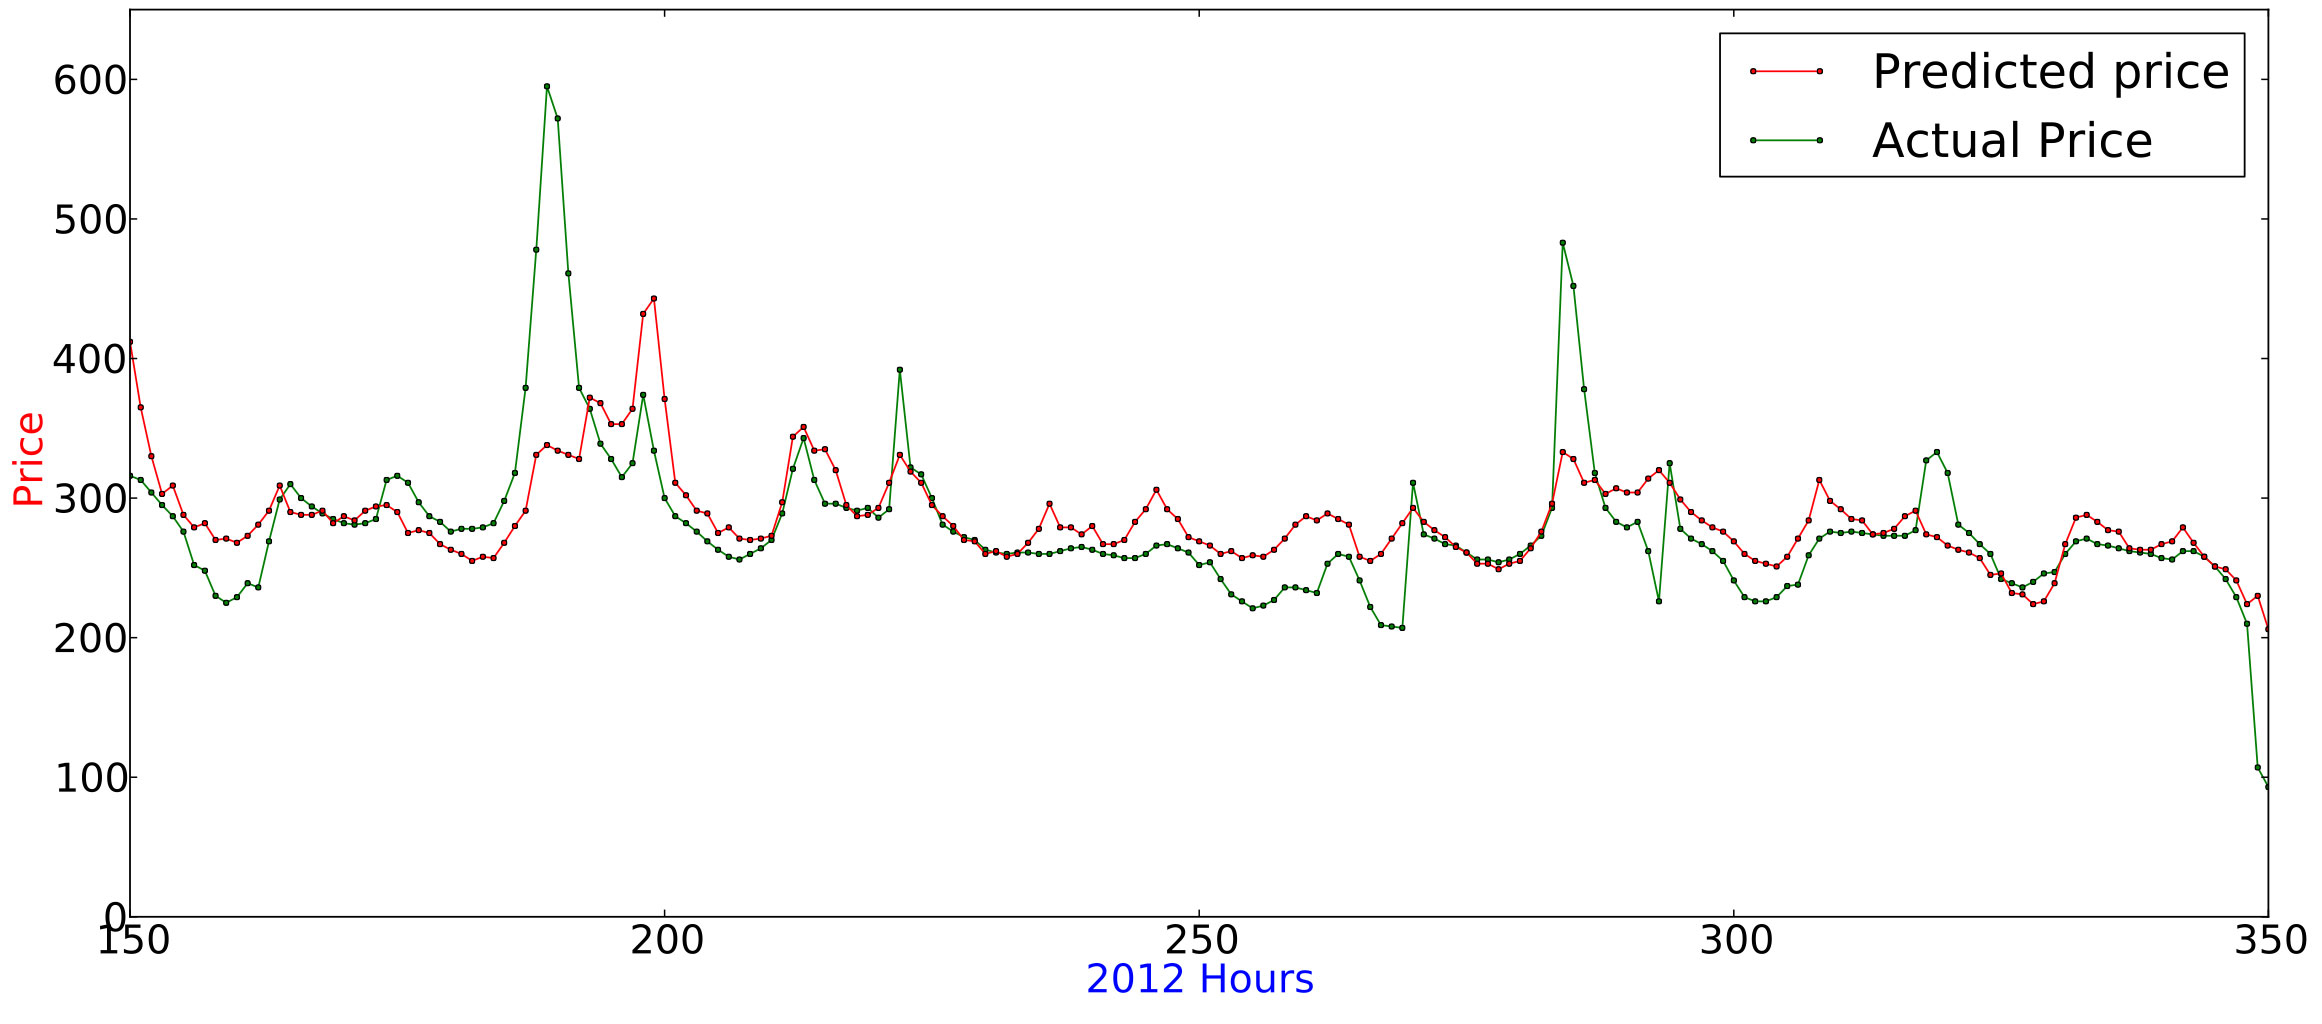
\includegraphics[width=\linewidth]{billeder/PriceExperimentalAnalysis/winter.jpg}
\caption{200 hours from winter}
\label{fig:Winter}
\end{figure}

\noindent We also see over fitting of the dataset when running more than 1800 epochs where the performance drops at least 10.26\% and gets worse with more epochs. Another thing to notice here is the time used to run the pruning algorithm and predict the next years data. We can see how the time rises when the number of epochs rises. Also the number of neurons in each layer have an influence on the time used to do the predictions (more neurons are equal to more time spent). Of course the time element is reduced when live data will be used real setting where the goal is to predict only one hour ahead. Even though we have included to show the time consumed because it says something about the inner workings of the system.

The following Figures \ref{fig:Winter}, \ref{fig:Spring}, \ref{fig:Summer} and \ref{fig:Fall} shows 200 hours taken from the four seasons. These have been included to show how well our predictions follow the real values.

Figure \ref{fig:Winter} shows a segment from the winter period. We can see that the spikes are hard to predict and these introduces a sizeable error margin in our dataset.

\begin{figure}[H]
\centering
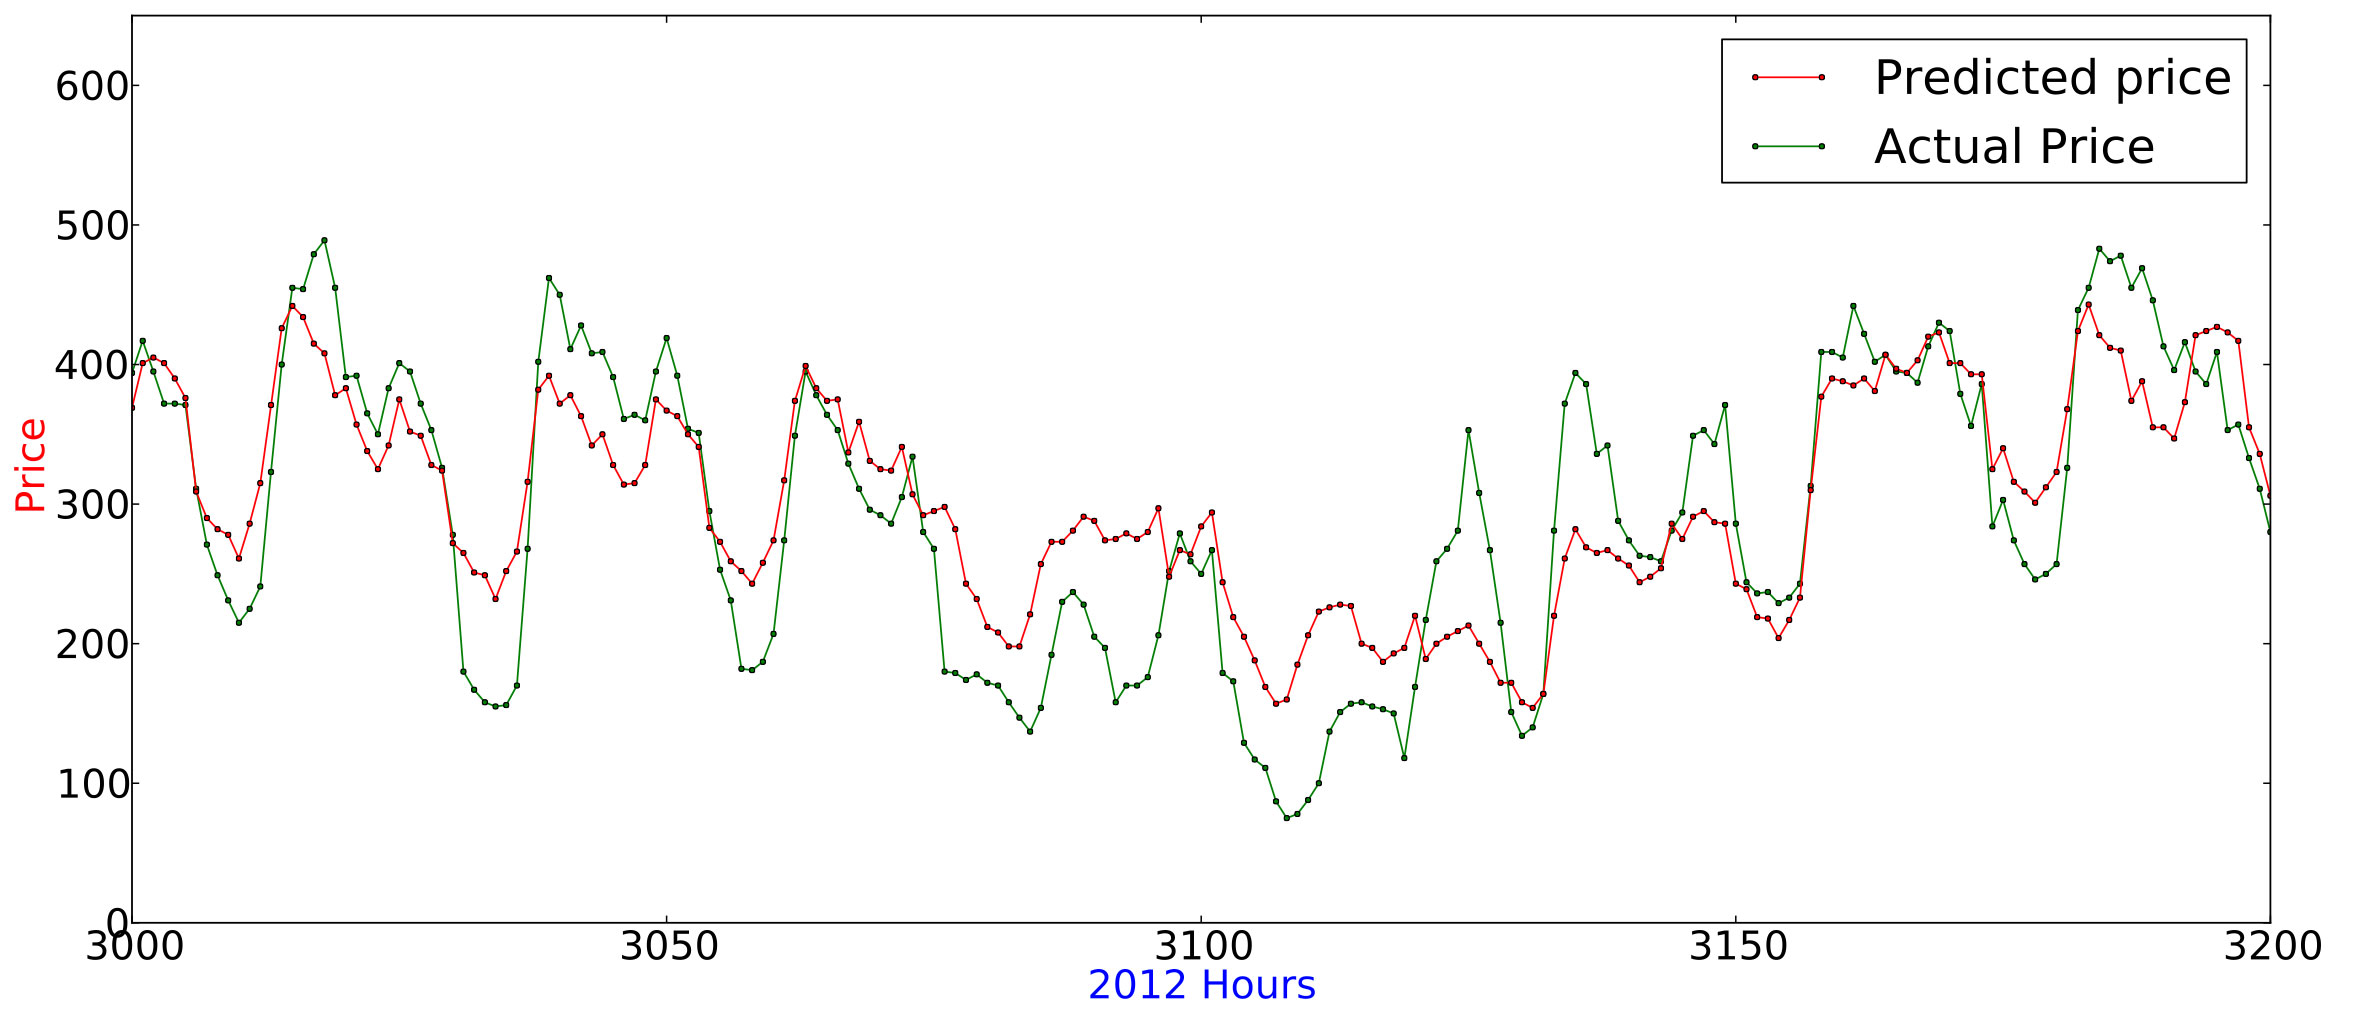
\includegraphics[width=\linewidth]{billeder/PriceExperimentalAnalysis/spring.jpg}
\caption{200 hours from spring}
\label{fig:Spring}
\end{figure}

Figure \ref{fig:Spring} shows a segments from the spring period. This curve is more volatile than the winter time and shows that we can follow this kind of curve behavior as well.

\begin{figure}[H]
\centering
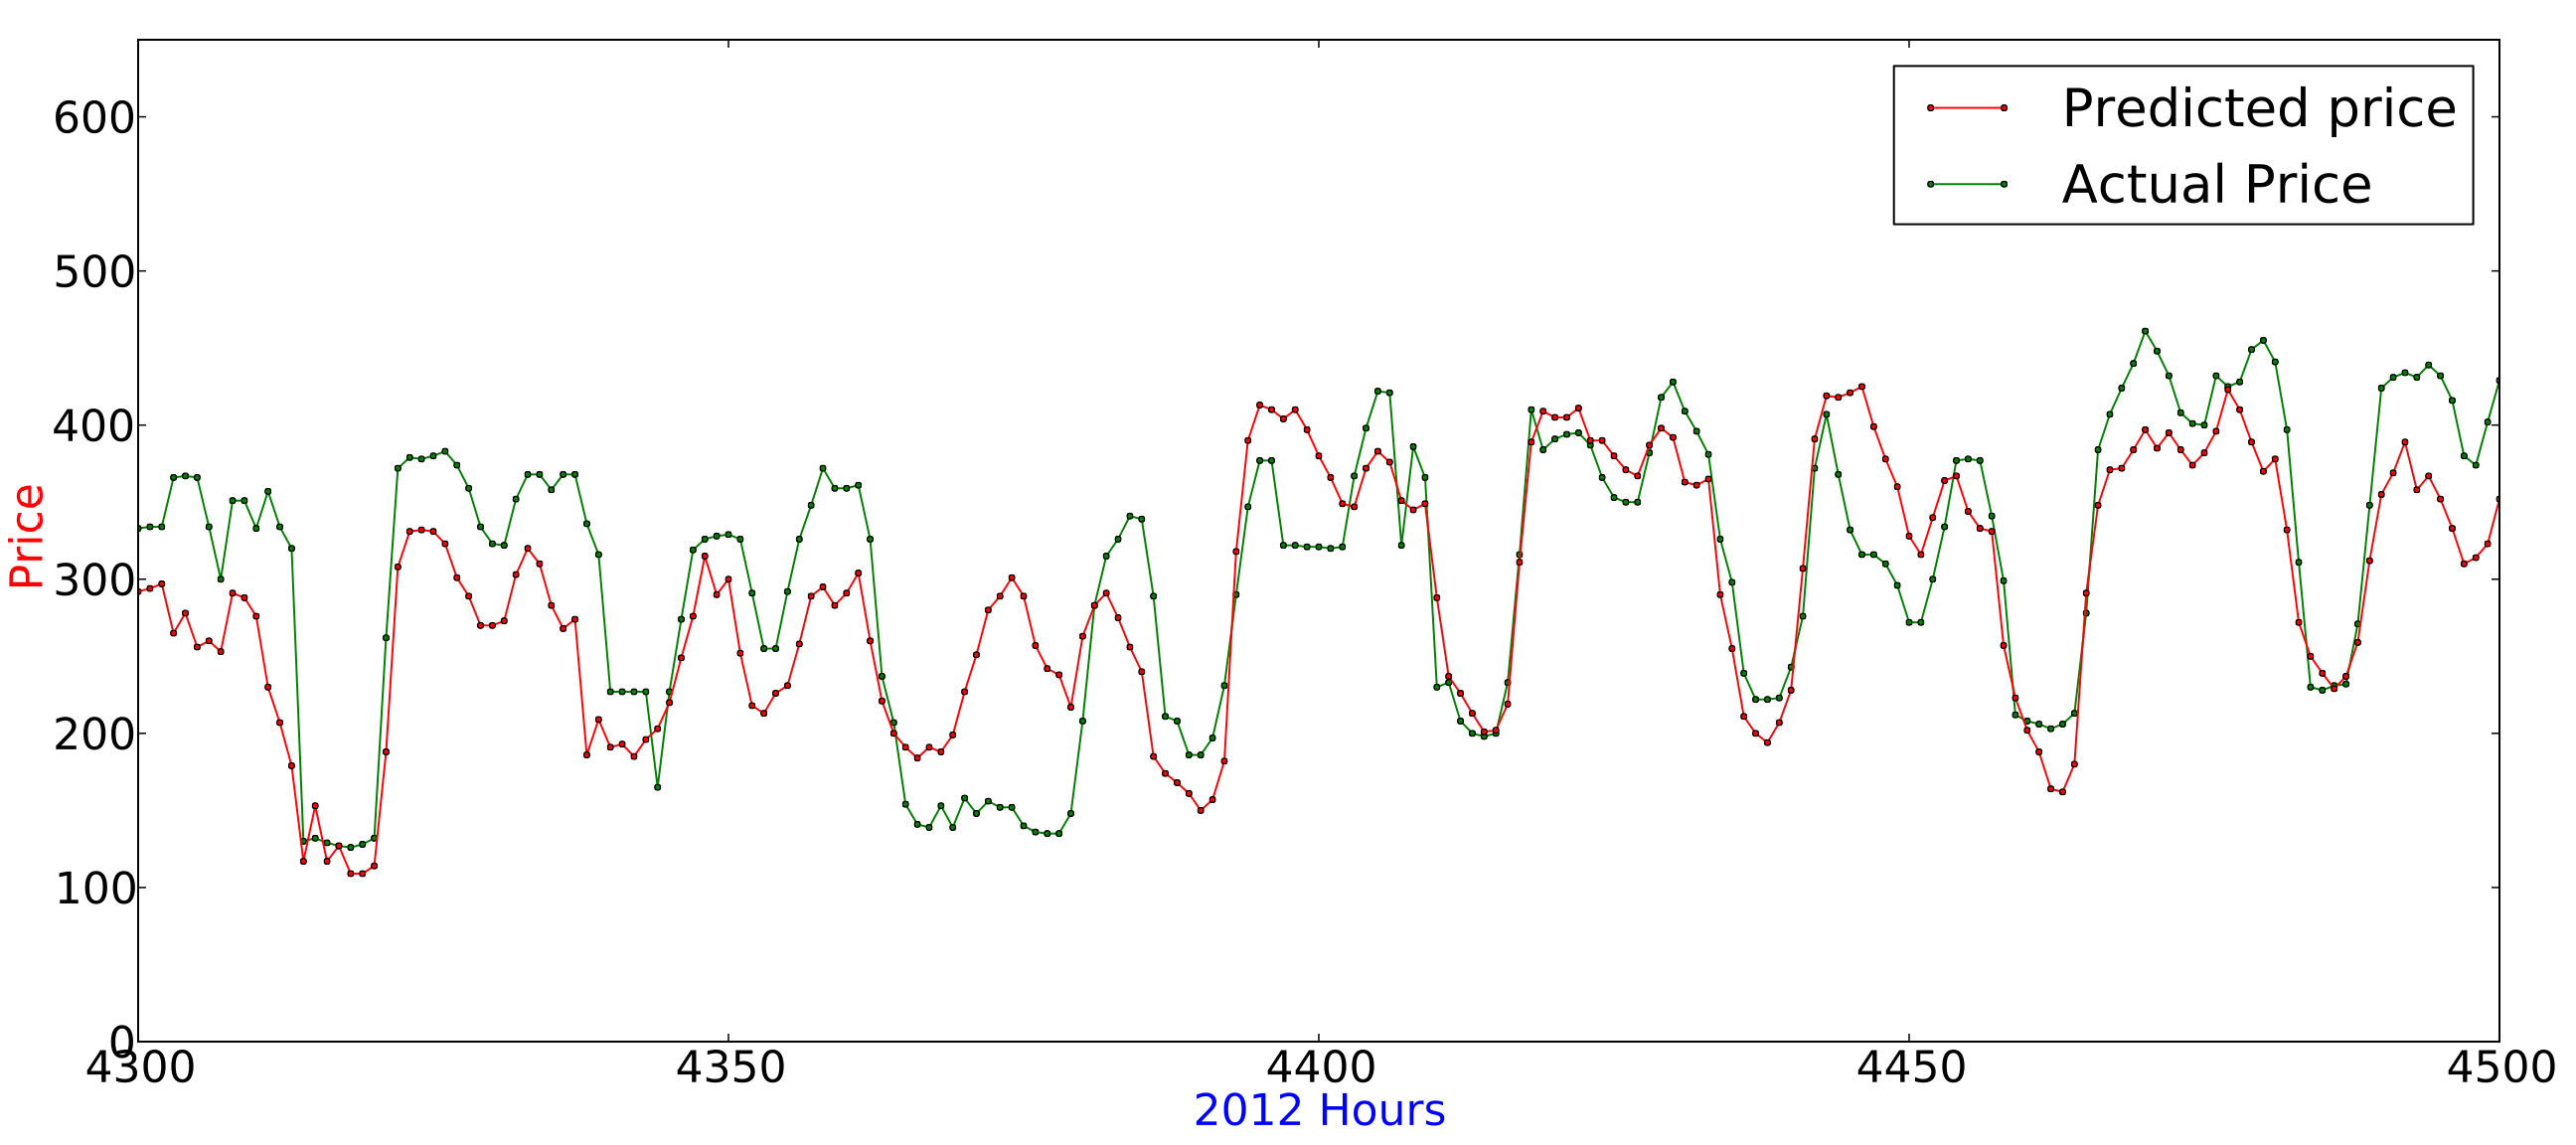
\includegraphics[width=\linewidth]{billeder/PriceExperimentalAnalysis/summer.jpg}
\caption{200 hours from summer}
\label{fig:Summer}
\end{figure}

Figure \ref{fig:Summer} shows the summertime. This graph is also very volatile and the predicted price follows the actual very well.

\begin{figure}[H]
\centering
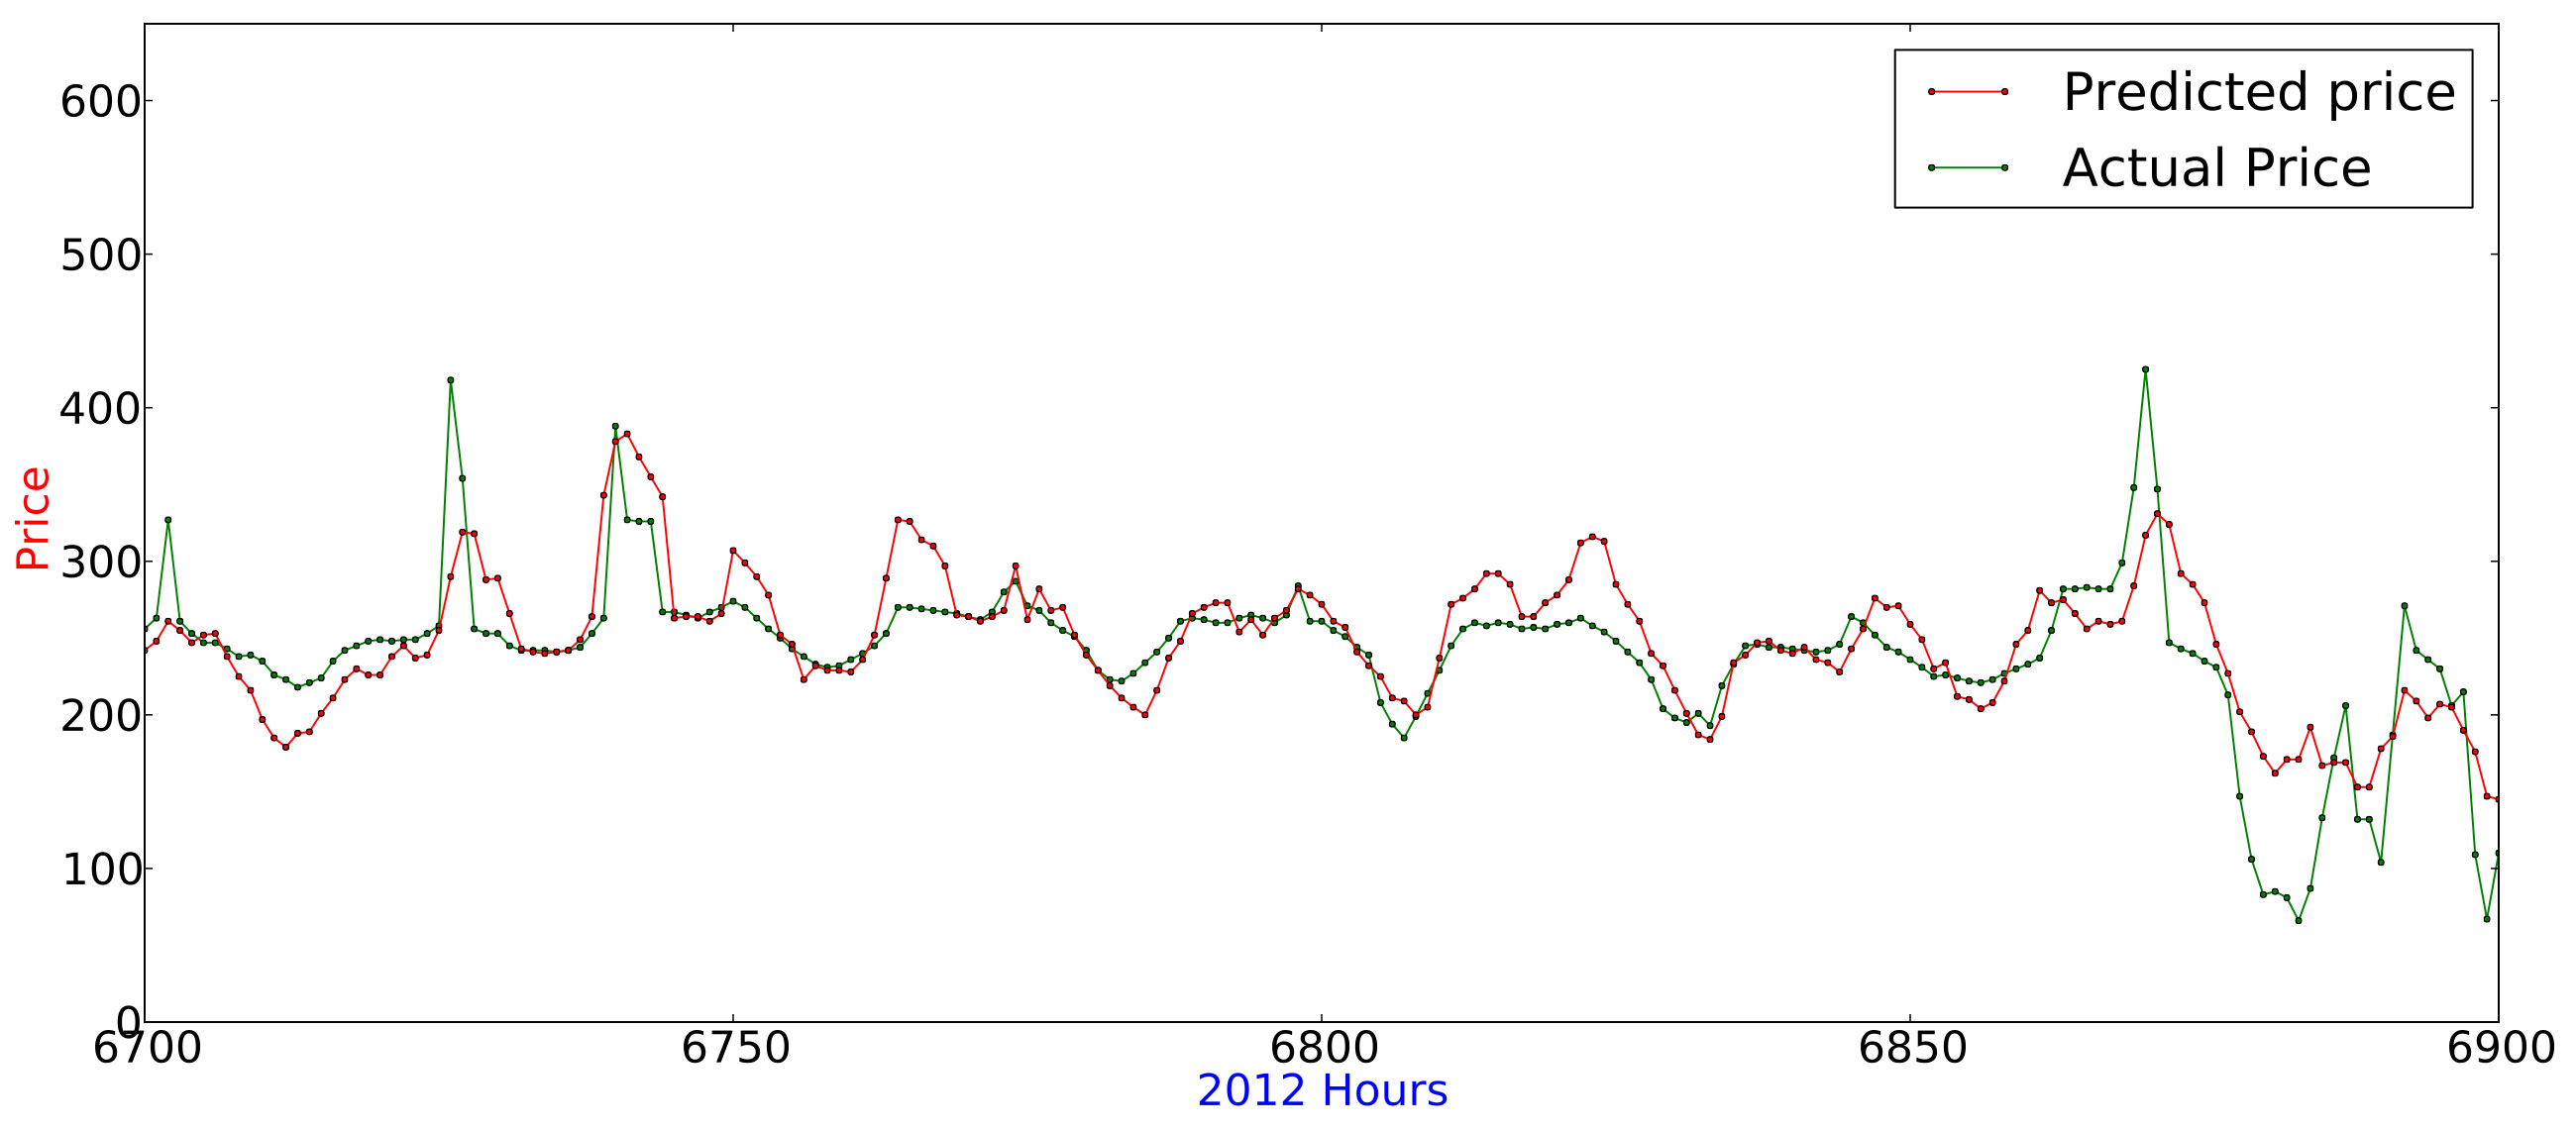
\includegraphics[width=\linewidth]{billeder/PriceExperimentalAnalysis/fall.jpg}
\caption{200 hours from fall}
\label{fig:Fall}
\end{figure}

In the last Figure \ref{fig:Fall} we see a segment from fall. It shows a more steady curve but also shows the difficulty that going from a flat curve to a volatile curve.

\subsubsection{Conclusion}
From this experiment we see that the optimal (for this input combination) training dataset size is half a year of data. We see an improvement of 6,46\% compared to the dataset size we have used in the prior experiments thus a better result from those experiments are expected if we use half a year of data instead of just a quarter of a year. The time consumed with this increase in the dataset would have doubled the time we used to conduct the trials. The time used to predict a full year are very close to a 1-to-1 correlation with the size of the dataset. 

The epochs used to train the network shows that values in the hundreds (100-900) dominate the top 10 results in Table~\ref{table:Epochs}. The best result is 500 epochs and shows an improvement over 200 epochs of 6.09\% which we used in prior experiments. These results also show how the time increases when the number of epochs increases. We still see a tendency where higher number of epochs results in more time consumed doing the experiment.

Of course these are not final and if something is changed in the input set then we have to retest what the best setup will be. The results reflect the best black optimization for our specific input combination and experimental setup. The dataset size and epochs are not necessarily (most likely not) transferable to other markets with other input parameters. 

\newpage
\subsection{Experiment Five - Step-Ahead Forecasting}
\label{sec:priceExperimentFive}
This experiment shows how the predictions behave when we increase the hours to use in step-ahead predictions. We have done a 1-hour ahead prediction and kept increasing the number until we hit 24 hours. We also conducted a test to see what the effects of changing the starting offset are.

\subsubsection{Variables}
This test were conducted using the best combination seen in Table ~\ref{table:Statistical1}. Giving us the following combination:
\begin{itemize}
	\item Price
	\item Demand
	\item Wind Speed
	\item Temperature
	\item Time of Day (Matrix)
	\item Day of Week (Matrix)
	\item Season of Year (Matrix)
	\item Skewness
	\item EWMA
\end{itemize}

The following parameters were tested:

\begin{itemize}
	\item Hours to use in step-ahead forecasting.
	\item Offset to start the prediction from.
\end{itemize}

\subsubsection{Hypothesis}
In this experiment we anticipate a decrease in MAE as we increase the number of hours the ANN has to predict. The reason for this is the elevation of error when we add more hours to predict ahead. The elevation comes from the last known price which will be the last predicted price (from hour 2 and onwards) thus elevating the error. The prediction of price relies in a great extend on the last-known price (see \ref{sec:Price}) and therefore it will have a significant effect on the price. We use the last-predicted price to simulate a real life setting where we have no idea what the next hours price will be and thus forcing us to rely on the last prediction when predicting the next hour.

We also expect to see that the MAE will change when we shift the offsets. The offsets decide where the first and (in most cases) best prediction will start. If these first predictions hit a good spot where the error margin will not rise as fast as other spots around it, then we will see a lower MAE.

\subsubsection{Results}
In Table \ref{table:XHoursAhead} we see the results from the hours ahead experiment. The MAE is linear with the number of hours ahead during the first 10 predictions. From there and on it is random what setup gives the worst result. From around 10 hours ahead the increase in MAE seems to be slowing down. This is because it is not only the last known price that dictates what the new prediction will be. The other input parameters (wind speed, time of day etc.) will also influence the price prediction. So when we hit a certain point in the prediction (which seems to be around 10 predictions ahead) the other input parameters will prevent the elevation of errors further. This can be seen in Figure~\ref{fig:24HoursAhead_elevationOfError} where the black lines denote 24 hours forecasts. We see in the 24 hours prediction (with the black box overlay) how the error is rising but when the prices start to fall so does the prediction. If it had been the last known price that dictated the next prediction then the predictions would have kept rising and so would the MAE.

\begin{figure}[H]
\centering
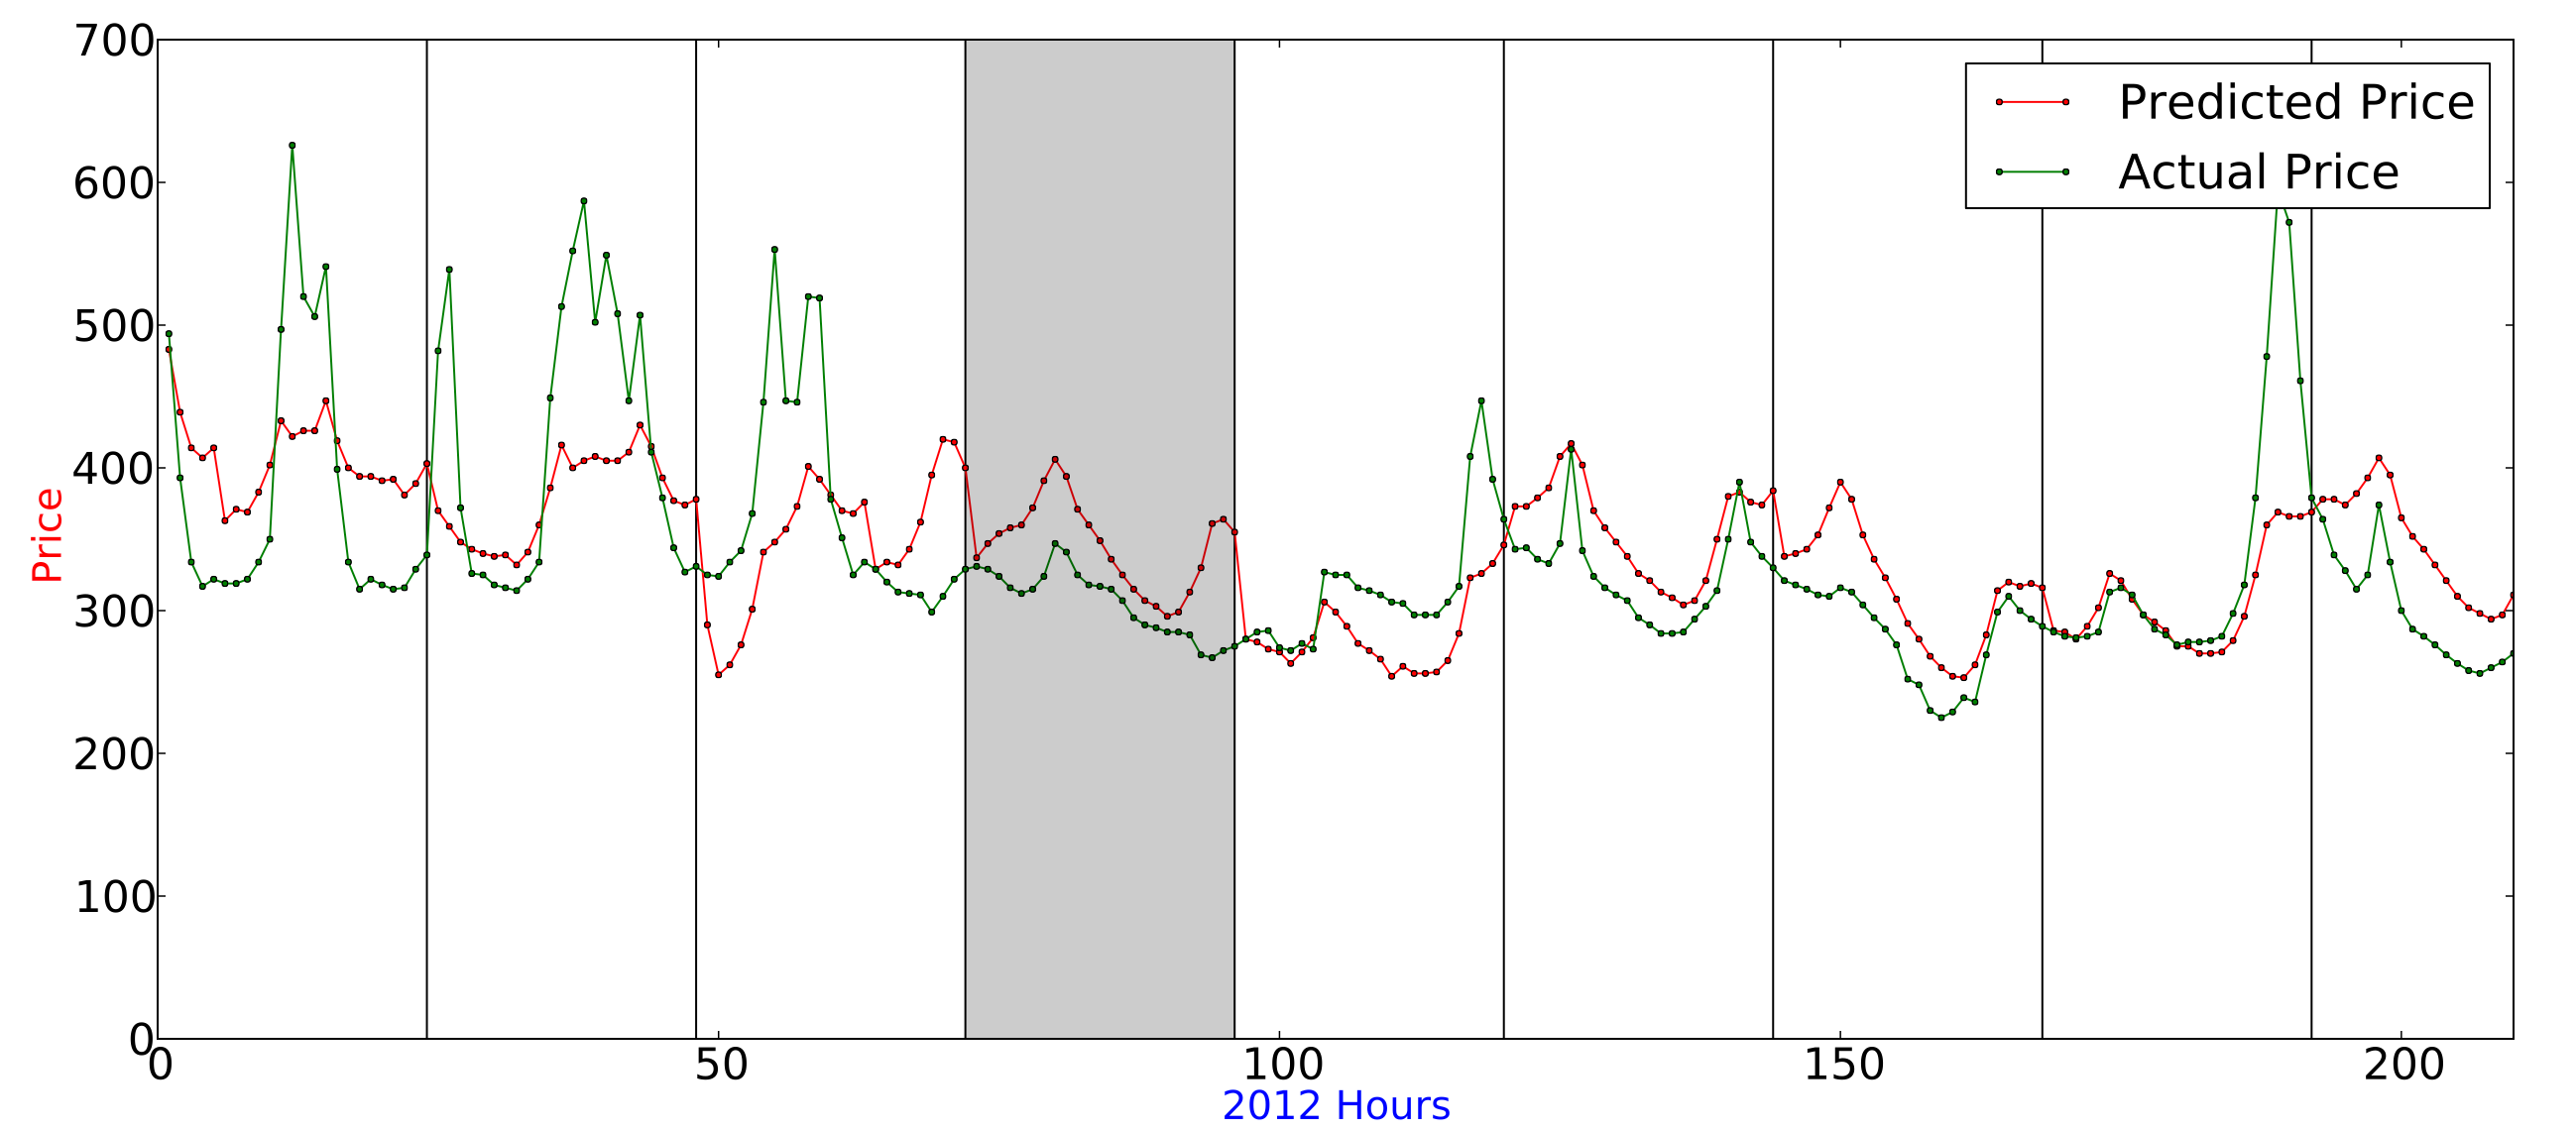
\includegraphics[width=\linewidth]{billeder/PriceExperimentalAnalysis/24HoursAhead_ElevationOfErrorExample.png}
\caption{Prediction of 24 hours ahead.}
\label{fig:24HoursAhead_elevationOfError}
\end{figure}

In the 2 hours ahead prediction seen in Figure~\ref{fig:2HoursAhead} we see how well the predictions are when we only predict 2 hours ahead. This is due to the limitation of the elevation of error which happens when we only have 1 hour dependent on an earlier prediction.

\begin{figure}[H]
\centering
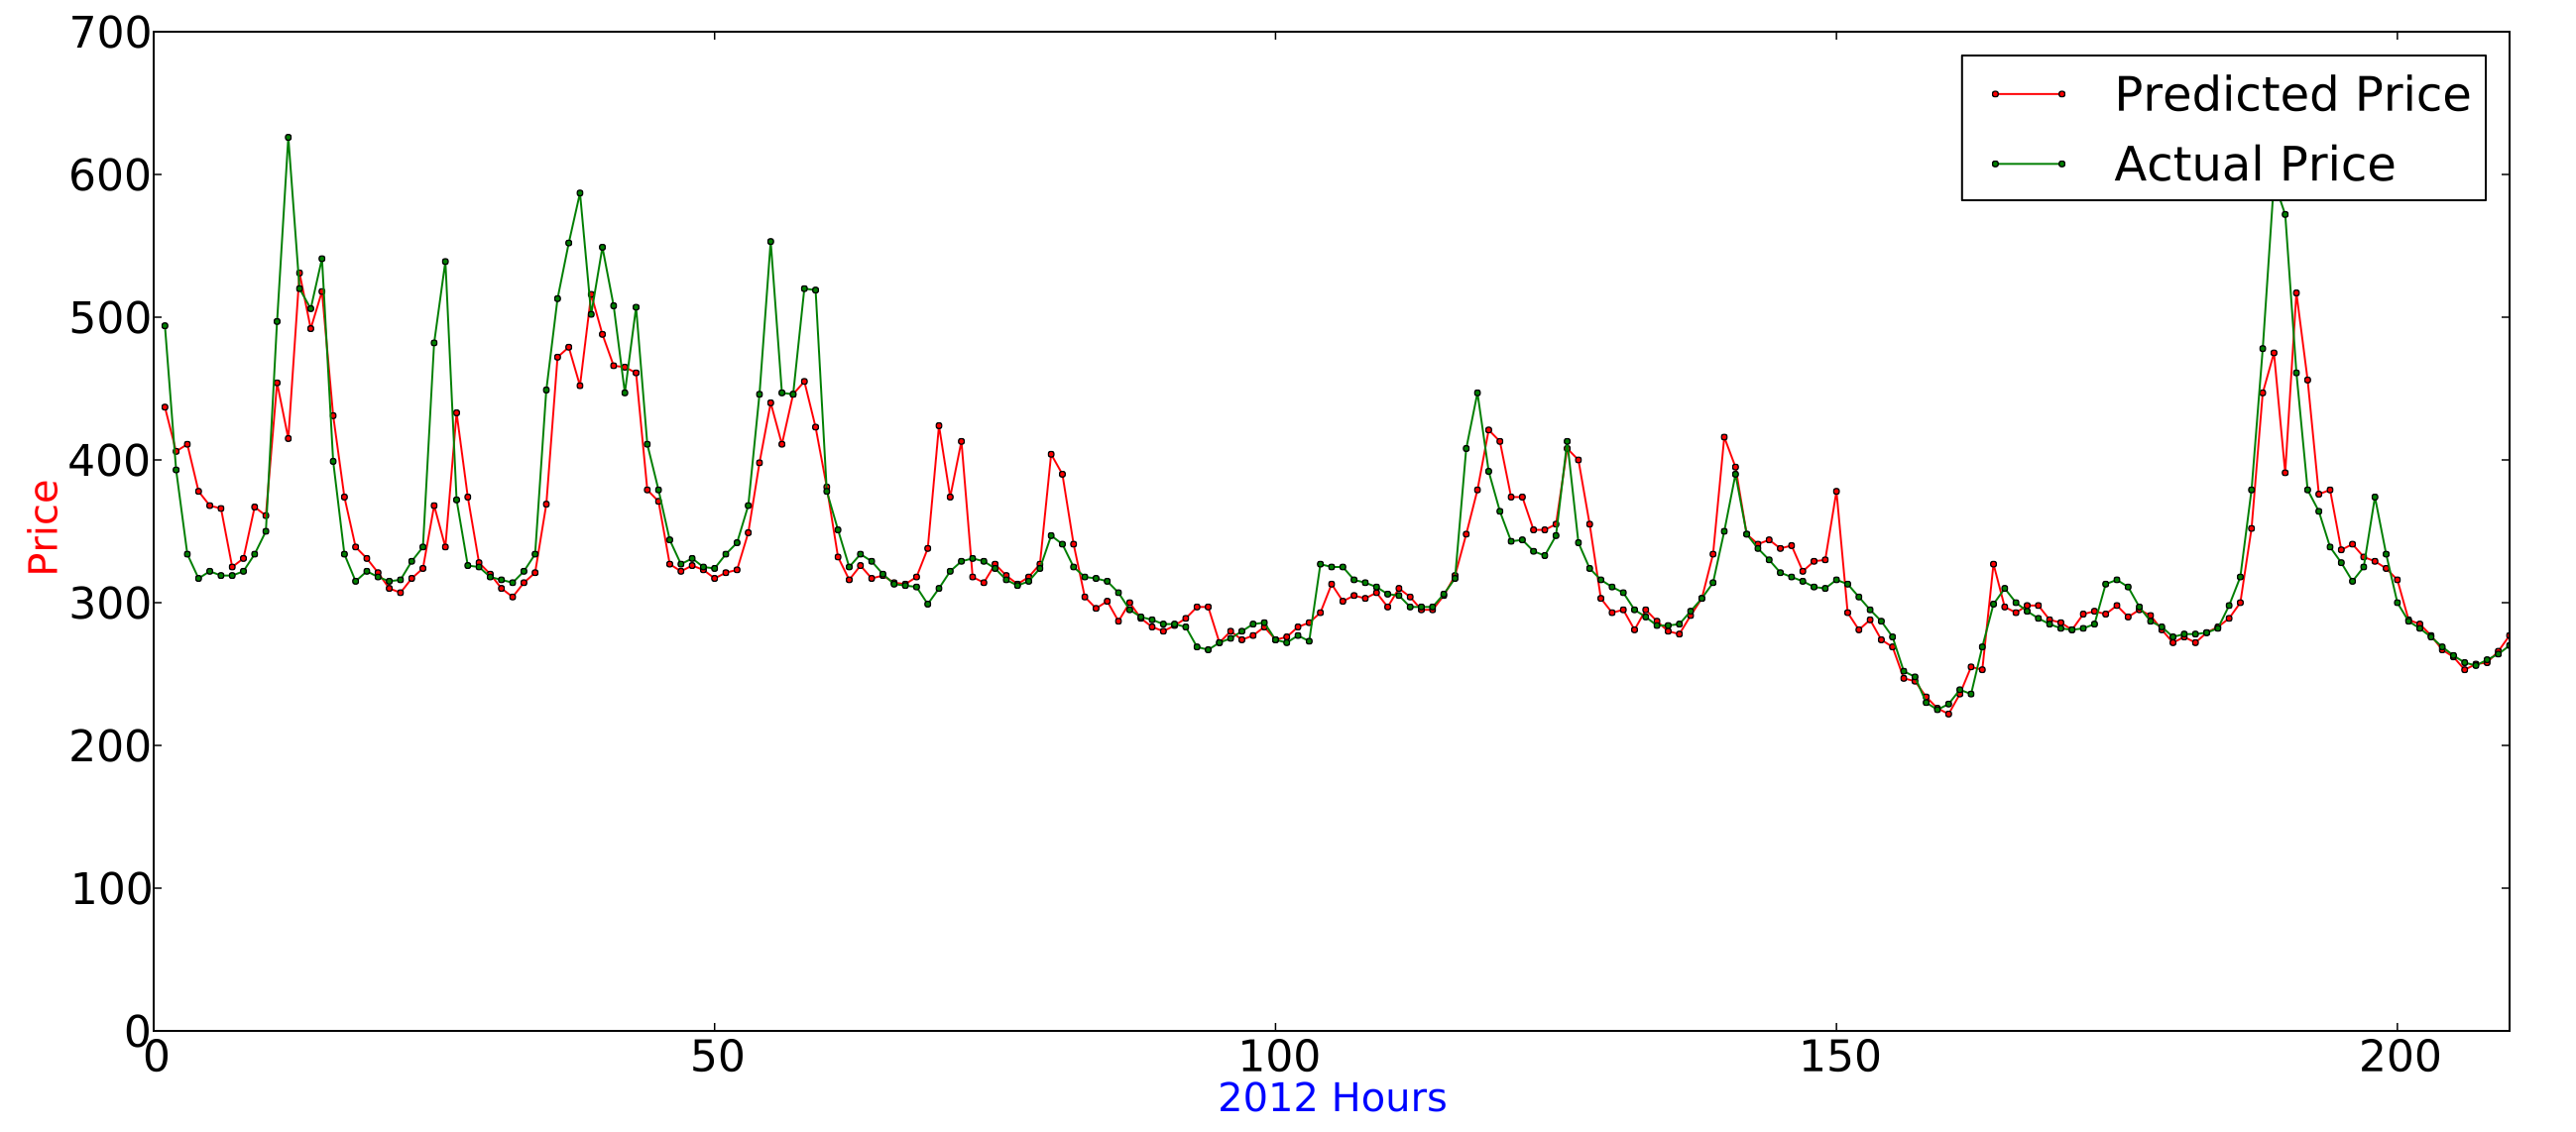
\includegraphics[width=\linewidth]{billeder/PriceExperimentalAnalysis/2HoursAheadForecast.png}
\caption{Prediction of 2 hours ahead}
\label{fig:2HoursAhead}
\end{figure}

In the 10 hours ahead predict seen in Figure~\ref{fig:10HoursAhead} we again see how the elevation happens. The black lines in the figure shows when we shift from one prediction cycle of 10 hours to the next. It is very clear in the figure how the predictions are corrected to fit the curve better every time we reset the prediction. From the beginning of every prediction cycle the next result will be based on correct data thus not relying on a potentially faulty prediction done earlier in the cycle.

\begin{figure}[H]
\centering
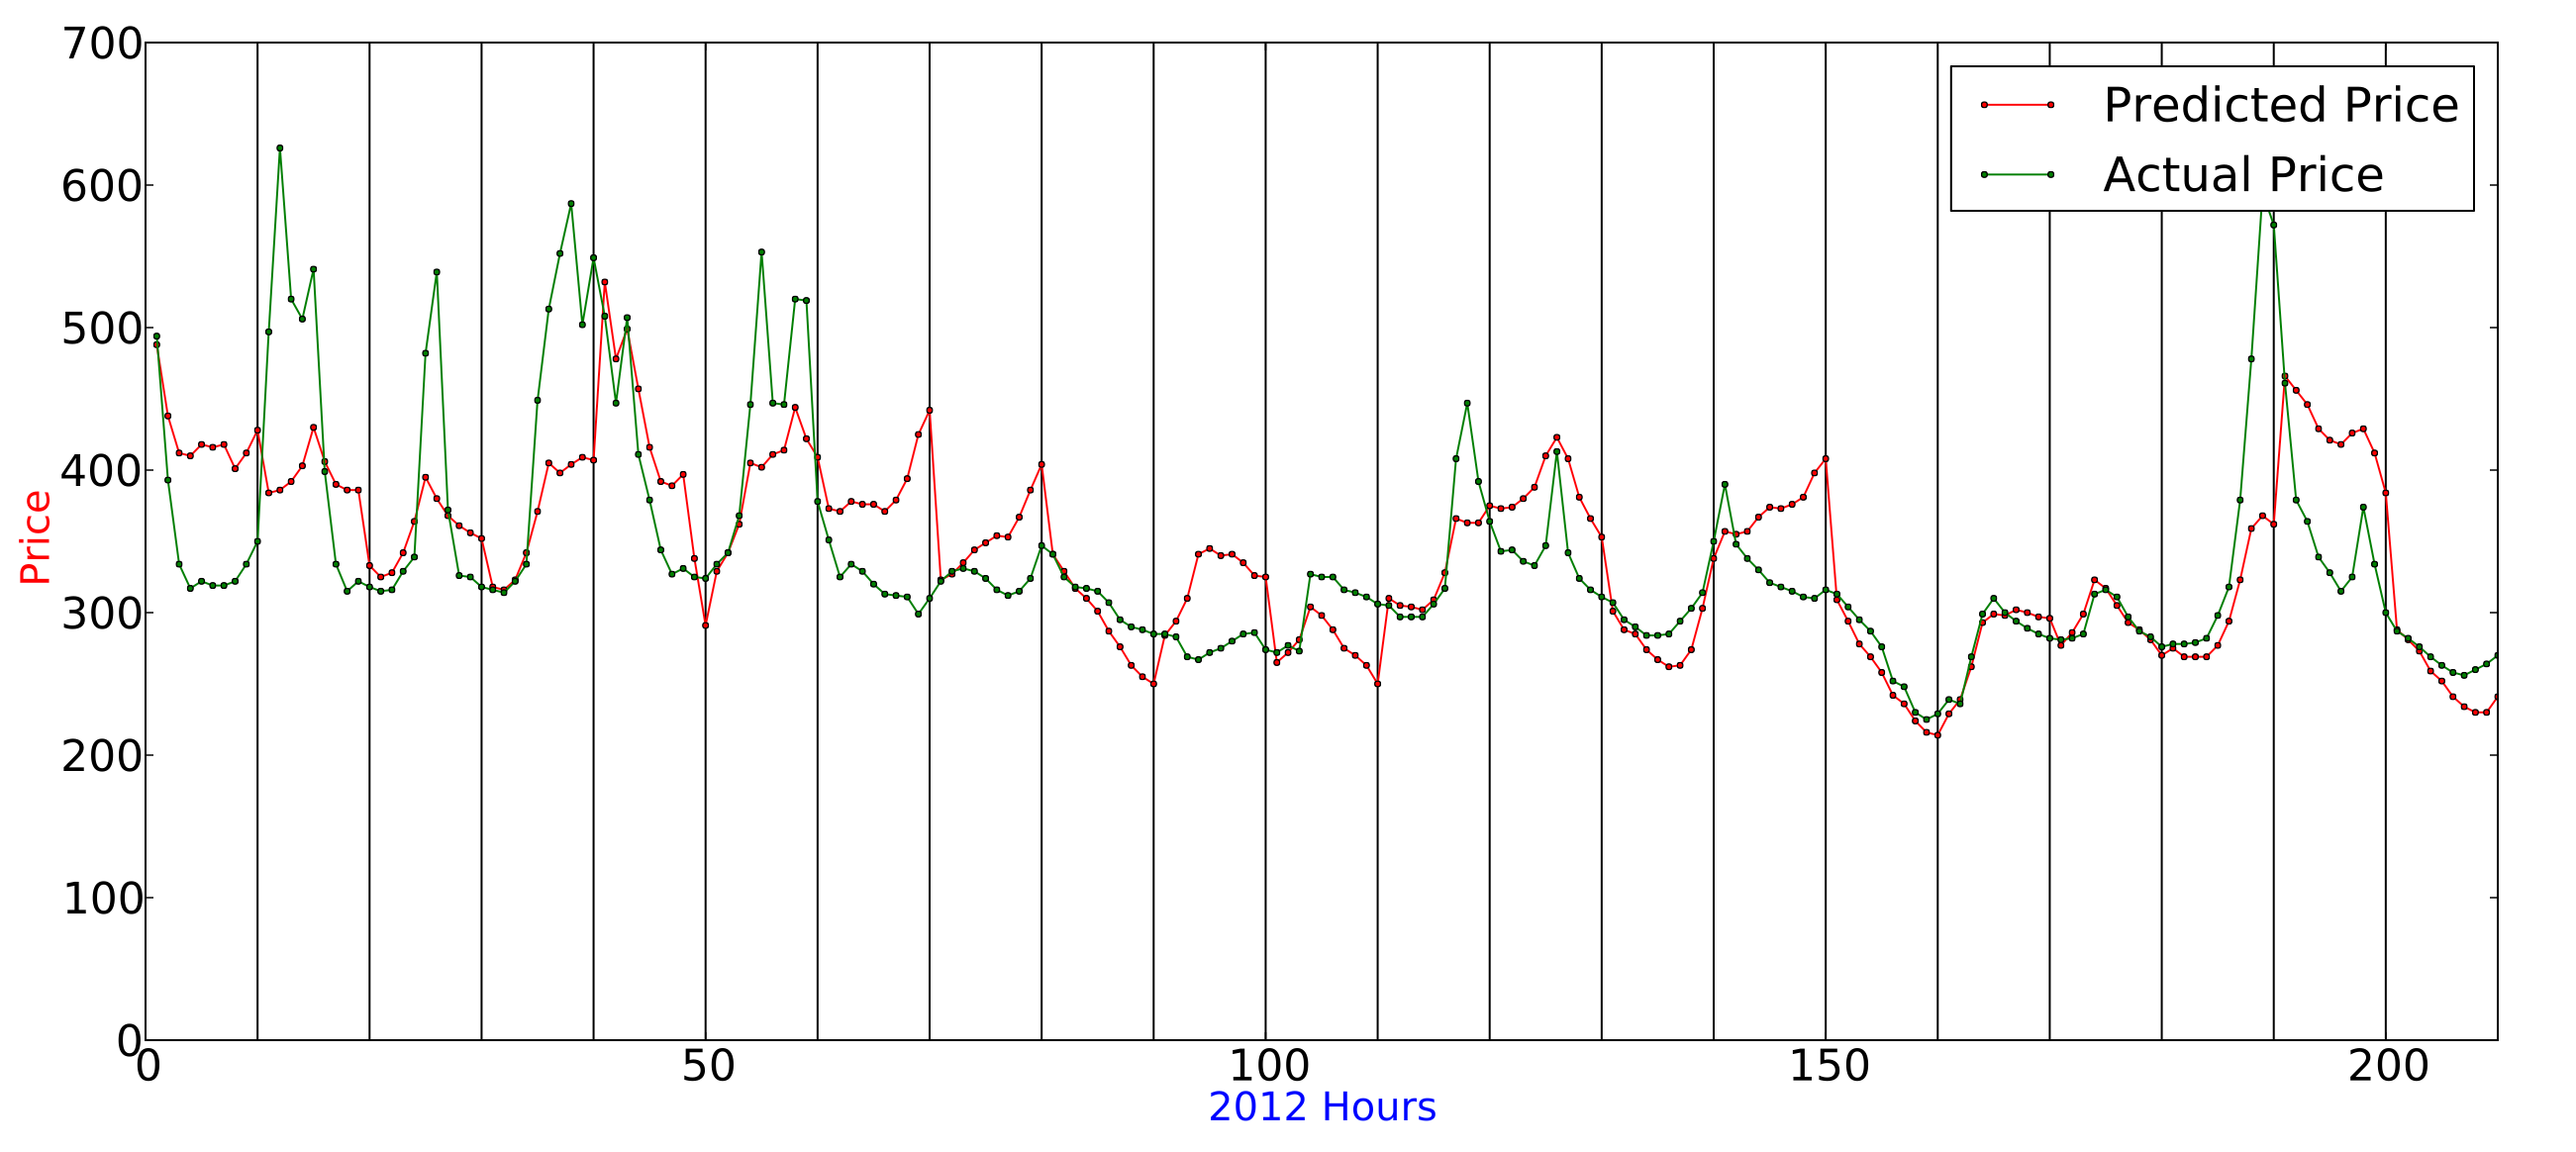
\includegraphics[width=\linewidth]{billeder/PriceExperimentalAnalysis/10HoursAhead.png}
\caption{Prediction of 10 hours ahead}
\label{fig:10HoursAhead}
\end{figure}

It is a bit surprising that the 1 hour ahead prediction shows a worse \% correct direction when it has a significantly better MAE. This might be because the 24 hours are better at following the trend of the curve.

\begin{table}[H]
\centering  % used for centering table
\resizebox{0.8\textwidth}{!}{
	\begin{tabular}{|c|c|c|c|c|c|c|c|c|}
	\hline
	\# & Hours ahead & Time(seconds) & H1 & H2 & \% CD & MAPE & MAE & \% Rank\\ [0.5ex] % inserts table 
	\hline  
	1  & 1   & 6790,62 & 12 & 10 & 60,1\% & 10,65\% & 27,87 & - \\ \hline
	2  & 2   & 3434,57 & 11 & 13 & 60,9\% & 12,58\% & 32,93 & 18,16\% \\ \hline
	3  & 4   & 1845,25 & 9  & 21 & 63,7\% & 13,91\% & 36,41 & 30,65\% \\ \hline
	4  & 3   & 2353,55 & 12 & 10 & 62,4\% & 14,14\% & 37,00 & 32,74\% \\ \hline
	5  & 5   & 1253,11 & 5  & 16 & 65,5\% & 14,44\% & 37,79 & 35,58\% \\ \hline
	6  & 7   & 963,92 & 10 & 6  & 65,7\% & 14,84\% & 38,84 & 39,37\% \\ \hline
	7  & 8   & 739,69 & 5  & 8  & 67,2\% & 14,92\% & 39,04 & 40,07\% \\ \hline
	8  & 11  & 623,99 & 5  & 15 & 67,9\% & 15,87\% & 41,52 & 48,96\% \\ \hline
	9  & 14  & 603,52 & 11 & 12 & 67,7\% & 16,97\% & 44,40 & 59,31\% \\ \hline
	10 & 12  & 607,08 & 6  & 13 & 65,2\% & 17,20\% & 45,02 & 61,51\% \\ \hline
	11 & 18  & 426,92 & 5  & 18 & 68,7\% & 17,22\% & 45,05 & 61,65\% \\ \hline
	12 & 6   & 1336,42 & 12 & 12 & 61,4\% & 17,37\% & 45,47 & 63,14\% \\ \hline
	13 & 13  & 551,3  & 8  & 9  & 67,1\% & 17,51\% & 45,83 & 64,42\% \\ \hline
	14 & 24  & 320,58 & 5  & 8  & 68,1\% & 17,80\% & 46,59 & 67,15\% \\ \hline
	15 & 9   & 844,39 & 12 & 5  & 63,5\% & 17,85\% & 46,72 & 67,6\% \\ \hline
	16 & 10  & 871,05 & 10 & 18 & 64,3\% & 18,21\% & 47,66 & 70,99\% \\ \hline
	17 & 21  & 446,34 & 8  & 18 & 66,5\% & 18,37\% & 48,09 & 72,52\% \\ \hline
	18 & 22  & 470,77 & 13 & 15 & 65,8\% & 18,58\% & 48,62 & 74,44\% \\ \hline
	19 & 17  & 584,8  & 13 & 15 & 62,8\% & 18,77\% & 49,13 & 76,28\% \\ \hline
	20 & 19  & 502,59 & 9  & 21 & 65,2\% & 19,07\% & 49,90 & 79,03\% \\ \hline
	21 & 23  & 429,65 & 17 & 4  & 64,7\% & 19,34\% & 50,62 & 81,63\% \\ \hline
	22 & 15  & 687,82 & 20 & 10 & 62,9\% & 19,36\% & 50,66 & 81,75\% \\ \hline
	23 & 16  & 534,67 & 10 & 12 & 64,4\% & 19,43\% & 50,84 & 82,39\% \\ \hline
	24 & 20  & 509,61 & 10 & 21 & 62,6\% & 19,70\% & 51,55 & 84,96\% \\ \hline
	\end{tabular}
}
\caption{The results from the hours ahead predictions.} % title of Table
\label{table:XHoursAhead} % is used to refer this table in the text
\end{table}

\begin{table}[H]
\centering  % used for centering table
\resizebox{0.8\textwidth}{!}{
	\begin{tabular}{|c|c|c|c|c|c|c|c|c|}
	\hline
	\# & Offset & Time(seconds) & H1 & H2 & \% CD & MAPE & MAE & \% Rank\\ [0.5ex] % inserts table 
	\hline 
	1  & 4   & 370,54 & 9  & 12 & 66,0\% & 17,82\% & 46,63 & - \\ \hline
	2  & 0   & 333,96 & 8  & 10 & 67,0\% & 17,99\% & 47,07 & 0,95\% \\ \hline
	3  & 8   & 364,68 & 8  & 12 & 66,8\% & 18,07\% & 47,29 & 1,41\% \\ \hline
	4  & 11  & 351,22 & 9  & 8  & 67,6\% & 18,09\% & 47,35 & 1,54\% \\ \hline
	5  & 14  & 358,79 & 8  & 11 & 66,9\% & 18,13\% & 47,45 & 1,75\% \\ \hline
	6  & 10  & 385,88 & 10 & 11 & 66,9\% & 18,14\% & 47,46 & 1,79\% \\ \hline
	7  & 21  & 339,93 & 8  & 9  & 68,6\% & 18,18\% & 47,58 & 2,04\% \\ \hline
	8  & 17  & 380,54 & 11 & 9  & 67,1\% & 18,30\% & 47,90 & 2,72\% \\ \hline
	9  & 1   & 345,99 & 7  & 15 & 68,4\% & 18,38\% & 48,11 & 3,18\% \\ \hline
	10 & 2   & 352,35 & 12 & 5  & 66,4\% & 18,74\% & 49,06 & 5,2\% \\ \hline
	11 & 12  & 406,33 & 13 & 11 & 65,5\% & 18,76\% & 49,09 & 5,28\% \\ \hline
	12 & 9   & 311,51 & 6  & 7  & 68,0\% & 18,78\% & 49,15 & 5,4\% \\ \hline
	13 & 13  & 410,08 & 13 & 11 & 65,5\% & 19,04\% & 49,84 & 6,87\% \\ \hline
	14 & 3   & 417,93 & 14 & 12 & 65,3\% & 19,13\% & 50,06 & 7,36\% \\ \hline
	15 & 19  & 404,45 & 11 & 12 & 65,7\% & 19,44\% & 50,87 & 9,1\% \\ \hline
	16 & 5   & 387,61 & 12 & 9  & 65,3\% & 19,52\% & 51,07 & 9,53\% \\ \hline
	17 & 20  & 404,6  & 7  & 24 & 65,3\% & 19,64\% & 51,41 & 10,25\% \\ \hline
	18 & 15  & 395,16 & 11 & 11 & 66,4\% & 19,80\% & 51,82 & 11,14\% \\ \hline
	19 & 16  & 409,38 & 13 & 10 & 64,5\% & 19,83\% & 51,91 & 11,32\% \\ \hline
	20 & 6   & 408,67 & 16 & 6  & 63,8\% & 19,84\% & 51,93 & 11,37\% \\ \hline
	21 & 22  & 448,74 & 17 & 9  & 64,6\% & 19,87\% & 52,00 & 11,52\% \\ \hline
	22 & 18  & 433,96 & 9  & 21 & 63,6\% & 19,96\% & 52,25 & 12,05\% \\ \hline
	23 & 23  & 349,56 & 8  & 10 & 67,5\% & 20,26\% & 53,02 & 13,7\% \\ \hline
	24 & 7   & 410,11 & 9  & 18 & 65,8\% & 20,50\% & 53,64 & 15,04\% \\ \hline
	\end{tabular}
}
\caption{The difference in MAE depending on the starting offset} % title of Table
\label{table:Offsets} % is used to refer this table in the text
\end{table}

In Table~\ref{table:Offsets} we see the results from the sliding window test. The entry with offset 0 is the same setup as prior experiments. The rest shows the difference in MAE when we shift where the 24 hours ahead predictions begin. We cover all possible offsets by doing 0-23 thus covering every offset from the first 24 hour prediction and onwards. From this experiment we show how much the right offset means for the total MAE in a years prediction. The biggest difference are between offset 4 and offset 7 with a difference of 15,04\%. These differences are connected to the elevation of error we talked about in the last result. If we hit the right spots where the elevation of error are not going to have a big impact this will lower the overall MAE thus giving us a better result.

\subsubsection{Conclusion}
In the hours ahead prediction we saw that the error margin was rising up until 10 hours ahead and from there only increasing slightly. This is because of the error margin not escalating infinitely but at some point will adapt to the changes in the other parameters pulling it in the right direction thus stopping the error from elevating further.

The offsets showed us a difference of 15,04\% from the best to the worst starting point. This difference in MAE is present because of how good a starting point the prediction will hit in general. The starting point is where the errors will start originating from; so if we can make the first prediction better the rest will in general also be better since we use the history of the curve to predict the next hourly price.

\newpage
\subsection{Concluding Remarks}
We conducted a series of experiments where we tested the parameters we identified in the electricity price analysis in Section~\ref{sec:ElectricityPriceAnalysis}. We have shown the results from five aspects of our modelled Feedforward Neural Network used for price predicting. We presented how the different parameters and setups change the output and accuracy of the ANN. In table~\ref{table:OverallImprovement} the best results from the experiments are presented and the overall improvement have been calculated to be 26.62\% from the initial tests to the best result in exp 3.

\begin{table}[H]
\centering  % used for centering table
\resizebox{0.8\textwidth}{!}{
	\begin{tabular}{|c|c|c|c|c|} % centered columns (7 columns)		
	\hline
	Exp 1 & Exp 2 & Exp 3 & Exp 4 & Overall improvement\\ [0.5ex] % inserts table 
	\hline 
	57.12 & 47,21 & 45,11 & 45.17 & 26.62\% \\ \hline
	\end{tabular}
}
\caption{The best results from the experiments and the overall improvement.} % title of Table
\label{table:OverallImprovement} % is used to refer this table in the text
\end{table}

The best result missed the target in average by a MAE of 45,11 DKK in an interval of 571.0 (lowest value 61.0 and highest 632.0) giving us a hit percentage of 7.90\%.

\begin{enumerate}
	\item Experiment one: This experiment showed how the different input parameters influenced the accuracy of the ANN and how important it is to select the right inputs. We also experimented with the format of the inputs; which we either represented as a matrix or a single input node. The best combination from this test is what we based the rest of the tests on. The best test result gave us the combination of last known price, demand, wind speed, temperature, the time of the day, the day of the week and the season of the year.
	\item Experiment two: We experimented with trimming and showed the benefits from trimming the dataset and the possible loss of accuracy on the upper and lower bound of the dataset. It only makes sense to trim the top and bottom of the dataset if extreme outliers are apparent in the dataset. We saw in the wind production experiment two~\ref{sec:windProdExperimentTwo} how trimming the dataset can have a negative effect on the outcome if the dataset does not contain extreme outliers. Trimming improved the price prediction by 20.99\% compared to the results from experiment one.
	\item Experiment three: This experiment shows the effect of adding calculated inputs to the ANN and how it improves the predictions. The calculated inputs improved the prediction of the results by 4.54\% and contained the historical volatility and the skewness inputs. We also tested scattered prices where the ANN on its own makes the connections between the historical prices and the output. These were only effective on the simplest of the datasets (price and demand) but did not have any effect on the best combination from experiment one.
	\item Experiment four: Here we tested different black box optimizations such as number of epochs used to train the network and size of the dataset. The best result here gave us 45,17 which were 0.13\% worse than experiment three but this is probably because of the randomness factor that will always have an influence when working with predictions.
	\item Experiment five: Shows how the ANN is affected by changing the number of hours ahead it has to predict. The error margin increases quite a lot when we add more hours ahead to predict. This is because of the dependency on the last hours price; which for each hour predicted might add more error to the calculations. We also showed the influence of what offset we start the predictions from. It shows how a good starting position can improve the results by 15.04\% from the worst to the best starting offset.
\end{enumerate}